%% elsarticle-based draft
%% Target: Fluid Phase Equilibria / Industrial & Engineering Chemistry Research
%% Compilation: pdflatex main && bibtex main && pdflatex main && pdflatex main

\documentclass[preprint,12pt,authoryear]{elsarticle}

\usepackage{amsmath,amssymb}
\usepackage{booktabs}
\usepackage{graphicx}
\usepackage{subcaption}
\usepackage{hyperref}
\usepackage{xcolor}
\usepackage{multirow}
\usepackage{siunitx}
\usepackage{algorithm}
\usepackage{algpseudocode}
\usepackage[left=1.5cm, right=1.5cm, top=2.5cm, bottom=2.5cm]{geometry}
\usepackage{lineno}
\modulolinenumbers[5]

\journal{Fluid Phase Equilibria}

%% ============================================================
\begin{document}

\begin{frontmatter}

\title{Fast and Robust Phase Equilibrium Computation for CO$_2$ + H$_2$O + NaCl Mixtures
       Using the Electrolyte Cubic-Plus-Association Equation of State}

\author[ohio]{Joachim Moortgat\corref{cor1}}
\ead{moortgat.1@osu.edu}
\author[unicamp]{Felipe Mour\~{a}o Coelho}
\author[rice]{Abbas Firoozabadi}
\cortext[cor1]{Corresponding author}
\affiliation[ohio]{organization={School of Earth Sciences, The Ohio State University},
             addressline={125 South Oval Mall},
             city={Columbus},
             state={OH},
             postcode={43201},
             country={USA}}
\affiliation[unicamp]{organization={Faculdade de Engenharia Qu\'{i}mica,
             Universidade Estadual de Campinas (UNICAMP)},
             city={Campinas-SP},
             postcode={13083-852},
             country={Brazil}}
\affiliation[rice]{organization={Rice University},
             city={Houston},
             state={TX},
             postcode={77005},
             country={USA}}

\begin{abstract}
We present an open-source Python implementation of phase stability and flash calculations for
 CO$_2$ + H$_2$O + NaCl mixtures using the electrolyte Cubic-Plus-Association (eCPA) equation
of state recently parameterized by \citet{Coelho2025}.
Starting from the eCPA thermodynamic framework, we developed (i) a generalized salt-free CPA flash
routine with Michelsen tangent-plane distance (TPD) stability tests and successive-substitution
iterations (SSI), which we validated for the CO$_2$ + H$_2$O binary; (ii) an extension to the
full ternary system including NaCl; and (iii) a precomputed four-dimensional solution table
spanning $T = 283$--$728$\,K, $P = 1$--$1500$\,bar, CO$_2$ overall mole fraction $z = 0.05$--$0.90$,
and NaCl molality $m_s = 0$--$6$\,mol\,kg$^{-1}$, enabling warm-started flash calculations that
are 3.2$\times$ faster than cold-start SSI.
Validation against $>$~1100 experimental data points shows average absolute relative errors (AARE)
of 8.2\% for CO$_2$ solubility in water, 6.9\% for CO$_2$ solubility in brine (603 converged points, $T = 278$--$623$\,K), and 0.33\% for
aqueous-phase density after optimization of a Péneloux volume shift for water
($c_{\text{H}_2\text{O}} = 0.11$\,cm$^3$\,mol$^{-1}$).
All source code is released under an open-source license and described in the Supplemental Information.
\end{abstract}

\begin{keyword}
CO$_2$ sequestration \sep eCPA equation of state \sep phase stability \sep flash calculation \sep
reservoir simulation \sep Péneloux volume shift \sep open-source
\end{keyword}

\end{frontmatter}

\linenumbers

%% ============================================================
\section{Introduction}
\label{sec:intro}

Geological storage of CO$_2$ in saline aquifers and depleted hydrocarbon reservoirs is one
of the most important near-term options for large-scale carbon capture and storage
\citep{Metz2005, Orr2004}.
Geothermal energy extraction presents a second and equally compelling application:
enhanced geothermal systems and hydrothermal reservoirs operate at temperatures well above
500\,K, where CO$_2$ can serve as a working fluid or co-migrate with brine, and where the
phase behavior of the CO$_2$ + H$_2$O + NaCl system must be accurately described to model
fluid circulation, energy extraction efficiency, and mineral scaling.
In both applications, accurate modeling of CO$_2$+brine phase behavior is a prerequisite
for reliable reservoir simulation: the equilibrium compositions of the CO$_2$-rich and aqueous
phases govern injectivity, trapping efficiency, and caprock integrity, while accurate density
predictions are needed for fluid flow and pressure calculations.
The high-temperature range ($T > 500$\,K) is particularly relevant to geothermal applications,
motivating the wide temperature coverage of the present model.

The equilibrium of CO$_2$ with brine is challenging to model because it spans a wide range of
conditions---temperatures from near-ambient ($\sim$283\,K) to supercritical and hydrothermal
($>$600\,K), pressures from hydrostatic (1\,bar) to lithostatic ($>$1000\,bar), and salinities
from fresh water to near-saturation ($>$6\,mol\,kg$^{-1}$ NaCl)---and involves both association
interactions (hydrogen bonding in water), CO$_2$--water cross-association, and electrostatic
effects of dissolved ions.

Cubic-Plus-Association (CPA) equations of state \citep{Kontogeorgis1996} successfully combine
a cubic (Soave--Redlich--Kwong, SRK) repulsive/dispersion term with a Wertheim association
term \citep{Wertheim1984} and have been widely applied to systems with hydrogen-bonding fluids.
The electrolyte CPA (eCPA) extension \citep{MaribMogensen2015} adds Debye--Hückel and Born
electrostatic terms to describe ion--solvent and ion--ion interactions.
\citet{Coelho2025} recently parameterized eCPA for the CO$_2$ + H$_2$O + NaCl ternary system
with temperature-dependent binary interaction parameters and a CO$_2$--H$_2$O
cross-association term, achieving a 74\% reduction in CO$_2$ solubility error in brine
compared to the prior model of \citet{MaribMogensen2015} (AARE: 6.9\% vs.\ 26.6\% over
660 data points from 283 to 723\,K).

Despite the availability of well-parameterized thermodynamic models, practical use in reservoir
simulation has been limited by the lack of open, efficient phase equilibrium routines for the
ternary system.
Reservoir simulators need flash calculations that are both \emph{robust}---returning the correct
phase split across the entire physically relevant parameter space---and \emph{fast}---executing
in milliseconds per grid cell to be compatible with time-stepping over millions of cells.
Achieving this for an EoS as complex as eCPA (which requires iterative solution of both the
cubic compressibility equation and the nonlinear association equations) is non-trivial.

The present work makes the following contributions:
\begin{enumerate}
  \item A complete implementation of the full eCPA equation of state of \citet{Coelho2025},
        including all Debye--Hückel, Born, association, and permittivity terms,
        validated against the original parameterization over $T = 283$--$728$\,K.
  \item A generalized salt-free CPA flash routine with Michelsen tangent-plane distance
        (TPD) stability testing \citep{Michelsen1982a} and successive-substitution /
        Newton flash \citep{Michelsen1982b}, validated for the CO$_2$ + H$_2$O binary.
  \item An extension to the ternary CO$_2$ + H$_2$O + NaCl system, in which the
        equilibrium aqueous molality $m_s$ is determined self-consistently within the
        SSI loop, replacing an earlier robust but slow outer root-finding loop over
        molality.
  \item A precomputed four-dimensional ($T$, $P$, $z$, $m_s$) solution table with
        234{,}360 grid points covering $T = 283$--$728$\,K and $m_s = 0$--$6$\,mol\,kg$^{-1}$,
        and a fast warm-started flash that reduces iteration
        counts from $\sim$12 to $\sim$3 (3.2$\times$ wall-time speedup), suitable
        for integration into reservoir simulators.
  \item Several algorithmic and software-engineering optimizations: multi-core parallelisation
        (via Python \texttt{multiprocessing}) for solution-table construction, phase-envelope
        tracing, and stability mapping; temperature and salinity continuation within the table
        build to maximise convergence rates; a logarithmic pressure axis for the interpolation
        grid; and compact binary storage (NumPy NPZ for the solution table, Apache Parquet for
        validation output) to minimise I/O overhead.
  \item Systematic validation against experimental vapor--liquid equilibrium (VLE) and density data, and an
        optimized Péneloux volume shift for H$_2$O ($c_{\text{H}_2\text{O}} = 0.11$\,cm$^3$\,mol$^{-1}$)
        that reduces aqueous-phase density AARE from 0.76\% to 0.33\%, an original
        contribution beyond \citet{Coelho2025}.
  \item A minimal but complete IMPEC compositional reservoir simulator (TPFA,
        two-phase Darcy flow, Corey relative permeabilities) that integrates the fast
        eCPA flash and demonstrates $\sim$600 flash calls\,s$^{-1}$ on a 2500-cell
        grid, with a discussion of how the routine can be embedded in open-source
        simulators (MRST, OPM Flow, DuMu$^x$).
  \item Open-source release of all code and a precomputed solution table, described
        in the Supplemental Information.
\end{enumerate}


%% ============================================================
\section{Thermodynamic Framework}
\label{sec:eos}

\subsection{CPA equation of state}
\label{sec:cpa}

For the salt-free CO$_2$ + H$_2$O binary the residual Helmholtz energy per mole is
\begin{equation}
  A^r = A^{\text{SRK}} + A^{\text{assoc}},
  \label{eq:Ar_cpa}
\end{equation}
where $A^{\text{SRK}}$ is the Soave--Redlich--Kwong \citep{Soave1972} physical term and
$A^{\text{assoc}}$ is the Wertheim association term.

The SRK compressibility factor satisfies
\begin{equation}
  Z = \frac{v}{v-b} - \frac{a(T)}{RT}\frac{1}{v+b},
  \label{eq:Z_srk}
\end{equation}
where $v$ is the molar volume and $x_i$ is the mole fraction of species $i$;
$a(T) = \sum_i \sum_j x_i x_j (1-k_{ij})\sqrt{a_i a_j}$
and $b = \sum_i x_i b_i$ are the mixture attractive and co-volume parameters, respectively,
with sums over molecular species $i, j \in \{\text{H}_2\text{O},\, \text{CO}_2\}$
(and additionally Na$^+$, Cl$^-$ in the ternary system).
The Soave temperature dependence is
$a_i(T) = a_{0i}[1 + c_{1i}(1 - \sqrt{T/T_{c,i}})]^2$.
The Peng--Robinson (PR) equation of state \citep{PengRobinson1976} can serve equally well as
the cubic backbone; it has been used with cross-association in the CPA framework for
water-containing mixtures \citep{LiFiroozabadi2009}.
We follow \citet{Coelho2025} in using SRK throughout the present work.

The association term accounts for hydrogen bonding in water via the 4C scheme (two proton
donors and two proton acceptors), and includes cross-association between CO$_2$ and H$_2$O
\citep{LiFiroozabadi2009}.
The sum runs over molecular species only ($i \in \{\text{H}_2\text{O}, \text{CO}_2\}$);
ions carry no association sites:
\begin{equation}
  \frac{A^{\text{assoc}}}{NRT} = \sum_i x_i \sum_{A \in i}
    \left(\ln\chi^{A_i} - \frac{\chi^{A_i}}{2} + \frac{1}{2}\right),
  \label{eq:Aassoc}
\end{equation}
where $\chi^{A_i}$ is the fraction of molecules $i$ not bonded at site $A$:
\begin{equation}
  \chi^{A_i} = \frac{1}{1 + c \sum_j x_j \sum_{B \in j} \chi^{B_j}\,\delta^{A_iB_j}},
  \label{eq:chi}
\end{equation}
with $c = N_A/v$ the molecular number density ($N_A$ is Avogadro's number, $v$ the molar
volume) and $\delta^{A_iB_j}$ the association bonding volume between site $A$ on species
$i$ and site $B$ on species $j$.
The CO$_2$--H$_2$O cross-association strength is proportional to water self-association
\citep{Coelho2025}:
\begin{equation}
  \delta^{A_wB_c} = S_{cw}(T)\,\delta^{A_wB_w},
  \label{eq:Scw}
\end{equation}
where $S_{cw}(T)$ and the binary interaction parameter $k_{cw}(T)$ both follow quadratic
polynomials in $T/T_{c,c}$ ($T_{c,c} = 304.4$\,K, the CO$_2$ critical temperature), with
coefficients from \citet{Coelho2025} (Table~\ref{tab:binary_params}).

The temperature dependence of both $k_{cw}$ and $S_{cw}$ is essential because the CO$_2$+H$_2$O
system spans qualitatively different regimes across the validated temperature range.
Below $T_{c,c} = 304.4$\,K, CO$_2$ is a subcritical liquid and its fugacity is
governed primarily by vapor-pressure equilibrium.
Between $\sim$304\,K and $\sim$450\,K, CO$_2$ is supercritical and the aqueous solubility
decreases steeply with temperature.
Above $\sim$500\,K, the CO$_2$-rich phase acquires substantial water content
(up to 20--25\,mol\% at $T = 500$\,K and $P = 200$\,bar), making accurate modeling of both
phases equally important.
A single set of temperature-independent binary interaction parameters cannot simultaneously
describe all three regimes; the quadratic polynomial form of \citet{Coelho2025} provides
sufficient flexibility while remaining analytically tractable.

\subsection{eCPA equation of state}
\label{sec:ecpa}

For the ternary system, two electrostatic terms are added \citep{MaribMogensen2015}:
\begin{equation}
  A^r = A^{\text{SRK}} + A^{\text{assoc}} + A^{\text{DH}} + A^{\text{Born}},
  \label{eq:Ar_ecpa}
\end{equation}
where $A^{\text{DH}}$ and $A^{\text{Born}}$ are the Debye--Hückel and Born solvation
contributions, respectively.
The presence of NaCl (Na$^+$ + Cl$^-$ ion pair) modifies the dielectric constant $\varepsilon_r$
of the aqueous phase, which enters both electrostatic terms.
The permittivity is computed self-consistently from the Onsager--Kirkwood equation, linking
it to the Wertheim association fractions and the molecular dipole moments \citep{Coelho2025}.

Ion--molecule interactions in the SRK mixing rule are modeled via energy
parameters $\Delta U_{is}$ of the Non-Random Two-Liquid (NRTL) type with a temperature dependence of the form
\begin{equation}
  \Delta U_{is} = \Delta U_{is}^{\text{ref}} + \alpha_{is}R\!\left[
    \left(1 - \frac{T}{T_{is}^\alpha}\right)^2 - \left(1-\frac{T_{\text{ref}}}{T_{is}^\alpha}\right)^2
  \right],
  \label{eq:DeltaU}
\end{equation}
with $T_{\text{ref}} = 298.15$\,K and parameters from \citet{Coelho2025}.
All EoS parameters are listed in Tables~\ref{tab:pure_params} and \ref{tab:binary_params}.

\subsection{Density and Péneloux volume correction}
\label{sec:peneloux}

The molar volume in each phase is $V_m = ZRT/P$.
Cubic equations of state systematically over- or underpredict liquid densities.
The Péneloux volume translation \citep{Peneloux1982} corrects this without affecting
phase compositions (it is isofugacity-preserving):
\begin{equation}
  V_m^{\text{corr}} = V_m^{\text{EoS}} + \sum_i x_i c_i,
  \label{eq:peneloux}
\end{equation}
with the corrected density $\rho = M_{\text{mix}}/V_m^{\text{corr}}$.
\citet{Coelho2025} apply a shift $c_s = -53.5$\,cm$^3$\,mol$^{-1}$ to the NaCl species
to correct brine density.
In this work we additionally optimize a shift $c_{\text{H}_2\text{O}}$ for the water
component against 37 experimental aqueous-phase density points (Section~\ref{sec:density}).


%% ============================================================
\section{Phase Stability and Flash Computations}
\label{sec:flash}

\subsection{Initial implementation: outer Brent loop over aqueous molality}
\label{sec:brent}

As a first, robust implementation of the eCPA flash, we employed an outer Brent
root-finding loop over the equilibrium CO$_2$ molality $m_c$ [mol\,kg$^{-1}$] in the
aqueous phase.
The Brent method \citep{Brent1973} is a bracketed root-finding algorithm that combines
bisection with inverse quadratic interpolation, guaranteeing convergence within a
user-specified bracket without requiring a derivative.
At each trial molality, the aqueous-phase fugacity of CO$_2$ is evaluated using the eCPA EoS
and compared to its CO$_2$-rich phase counterpart; the Brent algorithm then bisects toward
the molality at which fugacities are equal.
This approach is self-bracketing and requires no initial guess for the full phase state
vector, making it highly robust.
However, each function evaluation requires solving the eCPA inner equations (cubic $Z$,
association fractions $\chi$, permittivity $\varepsilon_r$) via nested Newton solves,
making the outer loop expensive and ill-suited to the large number of evaluations required
in a parameter-space scan or a production reservoir simulator.
This motivated the development of the direct SSI approach described below.

\subsection{Michelsen tangent-plane distance stability test}
\label{sec:stability}

We implement the Michelsen tangent-plane distance (TPD) criterion \citep{Michelsen1982a}
to determine whether a mixture at given $(T, P, \mathbf{z})$ is stable (single phase) or
unstable (two-phase).
Here $\mathbf{z} = (z_{\text{H}_2\text{O}}, z_{\text{CO}_2})$ are the overall feed mole
fractions of the two molecular species (Na$^+$ and Cl$^-$ are not independent flash
variables; they enter through the molality-dependent fugacity coefficients).
The TPD function evaluated at trial composition $\mathbf{W} = (W_{\text{H}_2\text{O}}, W_{\text{CO}_2})$ is
\begin{equation}
  \text{TPD}(\mathbf{W}) = \sum_{i} W_i \left[\ln W_i + \ln \hat{\phi}_i(\mathbf{W}) - d_i\right],
  \label{eq:tpd}
\end{equation}
where the sum is over $i \in \{\text{H}_2\text{O}, \text{CO}_2\}$,
$d_i = \ln z_i + \ln \hat{\phi}_i(\mathbf{z})$, and $\hat{\phi}_i$ is the fugacity
coefficient.
A negative minimum of TPD indicates thermodynamic instability.
We initialize the stability SSI using two trial phases: a CO$_2$-rich phase and a water-rich
phase, following the approach of \citet{Michelsen1982a}.
For the eCPA system, both trial references use the CO$_2$-rich EoS for initialization, with
the aqueous stability metric $\text{TPD}_{\text{aq}}$ computed using aqueous-phase fugacity
coefficients.

In practice, the stability test is the most computationally expensive step ($\sim$30\,ms per
call), because it requires iterating the eCPA inner equations at each SSI step.
In the fast-flash algorithm described in Section~\ref{sec:fast_flash}, the stability test is
bypassed for conditions pre-classified as two-phase by the solution table, reducing this
overhead to zero for the vast majority of reservoir simulation cells.

\subsection{Successive-substitution isothermal flash}
\label{sec:ssi}

For two-phase conditions, we solve the equilibrium equations
\begin{equation}
  \hat{\phi}_i^{\text{aq}}(x_i, T, P) = \hat{\phi}_i^c(y_i, T, P), \quad i = \text{H}_2\text{O},\, \text{CO}_2,
  \label{eq:iso_eq}
\end{equation}
where $x_i$ and $y_i$ are the mole fractions of species $i$ in the aqueous and CO$_2$-rich
phases, respectively.
These are related through K-values $K_i = y_i / x_i$, which are iterated by modified successive substitution:
\begin{equation}
  \ln K_i^{(k+1)} = \ln K_i^{(k)} + \omega\left[\ln\hat{\phi}_i^{\text{aq}} - \ln\hat{\phi}_i^c\right]^{(k)},
  \label{eq:ssi}
\end{equation}
with damping factor $\omega \in (0, 1]$.
The CO$_2$-rich phase mole fraction $\beta$ (the fraction of total moles in the CO$_2$-rich
phase) is obtained at each step by solving the Rachford--Rice equation:
\begin{equation}
  \sum_{i} \frac{z_i(K_i - 1)}{1 + \beta(K_i - 1)} = 0,
  \label{eq:rr}
\end{equation}
where the sum is over $i \in \{\text{H}_2\text{O}, \text{CO}_2\}$ and
$z_i$ are the overall feed mole fractions.
Initial K-values are taken from Wilson's correlation unless a warm start is available from
the solution table (Section~\ref{sec:table}).

For cold-start SSI (without a table guess), a damping factor $\omega = 0.7$ is required to
avoid divergence; warm-started SSI (from a table guess with state-vector error $\lesssim 0.01$)
converges reliably with $\omega = 1.0$ in 3--4 iterations.

Within each SSI iteration, the eCPA fugacity coefficients for the aqueous phase require
simultaneous solution of three coupled equations: the cubic compressibility factor $Z_w$,
the relative permittivity $\varepsilon_r$, and the H$_2$O association fraction $\chi_{1w}$.
These quantities are mutually dependent --- $Z_w$ enters the molar volume and hence the
Debye--Hückel screening length; $\varepsilon_r$ modifies the electrostatic contribution to
the fugacity; and $\chi_{1w}$ feeds back into both the physical and association terms ---
requiring a three-variable Newton solve at each SSI step.
The CO$_2$-rich phase requires an analogous two-variable Newton solve for $Z_c$ and $\chi_{1c}$.
The coupling of these inner equations is the primary reason the eCPA flash is more expensive
per iteration than a conventional cubic EoS flash.

\subsection{Phase envelope}
\label{sec:envelope}

We trace the two-phase boundary (P--T locus at fixed $z$ and $m_s$) using the following
procedure:
\begin{enumerate}
  \item Scan a coarse grid of ($T$, $P$) points with the stability test to classify each
        cell as stable or unstable.
  \item Identify transitions between stable and unstable cells.
  \item Refine each transition to the phase boundary by bisection, using warm-started SSI
        to solve the flash at each trial point.
\end{enumerate}
To handle the large number of (T, P) combinations efficiently, the bisection at each
boundary point is executed in parallel across all available CPU cores.

\subsection{Fast flash for reservoir simulation}
\label{sec:fast_flash}

\subsubsection{Four-dimensional solution table}
\label{sec:table}

We precompute flash solutions on a four-dimensional grid $(T, P, z_{\text{CO}_2}, m_s)$ with:
\begin{itemize}
  \item $T$: 31 points from 283 to 728\,K (approximately uniform 15-K spacing),
        covering conditions from cold-basin CO$_2$ storage to hydrothermal and
        geothermal applications.
  \item $\log_{10}P$: 30 points from $\log_{10}(1)$ to $\log_{10}(1500)$ (log-uniform).
  \item $z_{\text{CO}_2}$: 18 points from 0.05 to 0.90.
  \item $m_s$ (NaCl molality): 14 points from 0.0 to 6.0\,mol\,kg$^{-1}$, spanning
        the full range of experimental data from dilute brine to near-saturation.
\end{itemize}
This gives $31 \times 30 \times 18 \times 14 = 234{,}360$ grid cells.
At each cell we store a 10-vector: the compressibility factors $(Z_w, Z_c)$,
H$_2$O mole fractions in each phase $(x_{1w}, x_{1c})$, permittivity $\varepsilon_r$,
H$_2$O association fractions $(\chi_{1w}, \chi_{1c})$ (using the notation of
Section~\ref{sec:ssi}), equilibrium NaCl molality $m_s^{\rm aq}$, and two auxiliary
quantities used for warm-starting.
We also store a scalar stability flag (two-phase or single-phase).

%The table is built in stages using ELV (equilibrium-liquid-vapor) direct solves throughout:
%the core grid ($T = 283$--$523$\,K, $m_s = 0.1$--$3.0$\,mol\,kg$^{-1}$) uses full cold-start
%flash (stability + SSI) with $T$-continuation and $m_s$-continuation fallbacks;
%the $m_s = 0$ slice uses bilinear interpolation from a high-resolution CO$_2$ + H$_2$O
%binary database;
%higher $m_s$ levels ($m_s > 3.0$\,mol\,kg$^{-1}$) use $m_s$-continuation from the converged
%$m_s = 3.0$ solution;
%and higher $T$ slices ($T > 523$\,K) use $T$-continuation from converged lower-$T$ solutions.
%All 234{,}360 cells in the final table are filled via nearest-neighbour interpolation for
%any non-converged cells (100\% coverage).

Table lookup uses a multilinear interpolant operating in $(T, \log_{10}P, z, m_s)$ space,
which is vectorized and evaluates in $<$1\,ms.

\subsubsection{Fast flash algorithm}
\label{sec:algorithm}

The fast flash routine operates as follows.
A query to the 4D interpolant yields an initial state vector (compressibility factors, phase
compositions, association fractions, and permittivity) together with a stability classification
(two-phase or single-phase).
If the interpolant classifies the condition as two-phase, the Michelsen stability test is
skipped and SSI is initialized directly from the table state vector with no damping ($\omega = 1.0$).
If the classification is single-phase or uncertain (for example, near the two-phase boundary
or for grid cells with low convergence quality), the full Michelsen TPD test is performed;
a stable result returns immediately without a flash, while an unstable result proceeds to SSI.
In either two-phase path, the warm-started SSI converges in 3--4 iterations because the
interpolated state vector is already within $\sim$1\% of the converged solution.
Should SSI fail to converge, a full cold-start with Wilson K-value initialization and damped
SSI ($\omega = 0.7$) provides a robust fallback.

The key insight enabling this strategy is that the solution surface --- the mapping from
$(T, P, z, m_s)$ to the equilibrium state vector --- is smooth and slowly varying except near
the two-phase boundary and the CO$_2$ critical point ($T_{c,c} = 304.4$\,K, $P_c = 73.8$\,bar).
A bilinear interpolant from a grid with 15\,K temperature spacing and log-uniform pressure
spacing (30 points per decade) therefore provides an excellent initial guess for the vast
majority of reservoir conditions.
The selective stability check further reduces cost: in a typical reservoir simulation, the
majority of grid cells are well within the two-phase region (injected CO$_2$ coexisting with
brine) and the interpolant stability flag can be trusted, while the expensive Michelsen test
is reserved for cells near boundaries where phase transitions occur.


%% ============================================================
\section{Validation}
\label{sec:validation}

\subsection{CO$_2$ + H$_2$O binary}
\label{sec:co2h2o}

We validate both the (new and tuned) salt-free CPA EOS and the eCPA EOS at $m_s = 10^{-4}$\,mol\,kg$^{-1}$
(effectively salt-free) against 631 experimental VLE data points compiled by \citet{Coelho2025}
for $T = 273$--$623$\,K.
Both phases are characterised: the CO$_2$ mole fraction in the aqueous phase $x_{\text{CO}_2}$ and
the H$_2$O mole fraction in the CO$_2$-rich phase $y_{\text{H}_2\text{O}}$.

Figure~\ref{fig:co2h2o_Tpanel} shows representative comparisons at six temperatures spanning
the validated range ($T = 298$--$523$\,K); results for all 35 temperatures are collected in
Fig.~\ref{fig:co2h2o_Tpanel_SI} in the Supplemental Information.
Table~\ref{tab:co2h2o_metrics} summarises the accuracy metrics.
Both CPA and eCPA achieve AARE $\approx 8$--$9\%$ for $x_{\text{CO}_2}$ and $\approx 23$--$25\%$
for $y_{\text{H}_2\text{O}}$; the somewhat larger error for the CO$_2$-rich phase is consistent with the
Coelho parametrization, which prioritizes brine conditions. The fact that the CPA and eCPA results, from independent codes, are essentially identical is an encouraging consistency validation. Note that the results in Figure~\ref{fig:co2h2o_Tpanel} are derived from our full phase stability plus flash, with a feed composition of 50 mol\% CO$_2$, whereas those in \citet{Coelho2025} are from simpler VLE computations (i.e.~without considering phase amounts). 

The most challenging conditions for both models are near the CO$_2$ critical point
($T_{c,c} = 304.4$\,K, $P_c = 73.8$\,bar), where the K-value gradients with pressure are steep
and small errors in fugacity coefficients translate to large errors in solubility.
Both CPA and eCPA show somewhat larger deviations in this region, consistent with the
general difficulty of describing near-critical behavior with a cubic EoS.
The parity plot in Fig.~\ref{fig:co2h2o_parity} confirms that neither model exhibits a
systematic bias across the full temperature range: the scatter around the 1:1 line is
largely random, with most points falling within the $\pm 20\%$ band.

\begin{table}[htb]
  \centering
  \caption{VLE accuracy metrics for the CO$_2$ + H$_2$O binary ($T = 273$--$623$\,K).
           AARE: average absolute relative error. $N$: number of experimental data points with converged CPA/eCPA solutions.}
  \label{tab:co2h2o_metrics}
  \begin{tabular}{lrrrr}
    \toprule
    Model & $N$ ($x_{\text{CO}_2}$) & AARE ($x_{\text{CO}_2}$) & $N$ ($y_{\text{H}_2\text{O}}$) & AARE ($y_{\text{H}_2\text{O}}$) \\
    \midrule
    CPA (salt-free)  & 460 & 8.9\% & 363 & 25.3\% \\
    eCPA ($m_s = 10^{-4}$) & 451 & 8.2\% & 357 & 23.0\% \\
    \bottomrule
  \end{tabular}
\end{table}

\begin{figure}[h!]
  \centering
  \newcommand{\sw}{0.47\textwidth}%
  \begin{subfigure}[t]{\sw}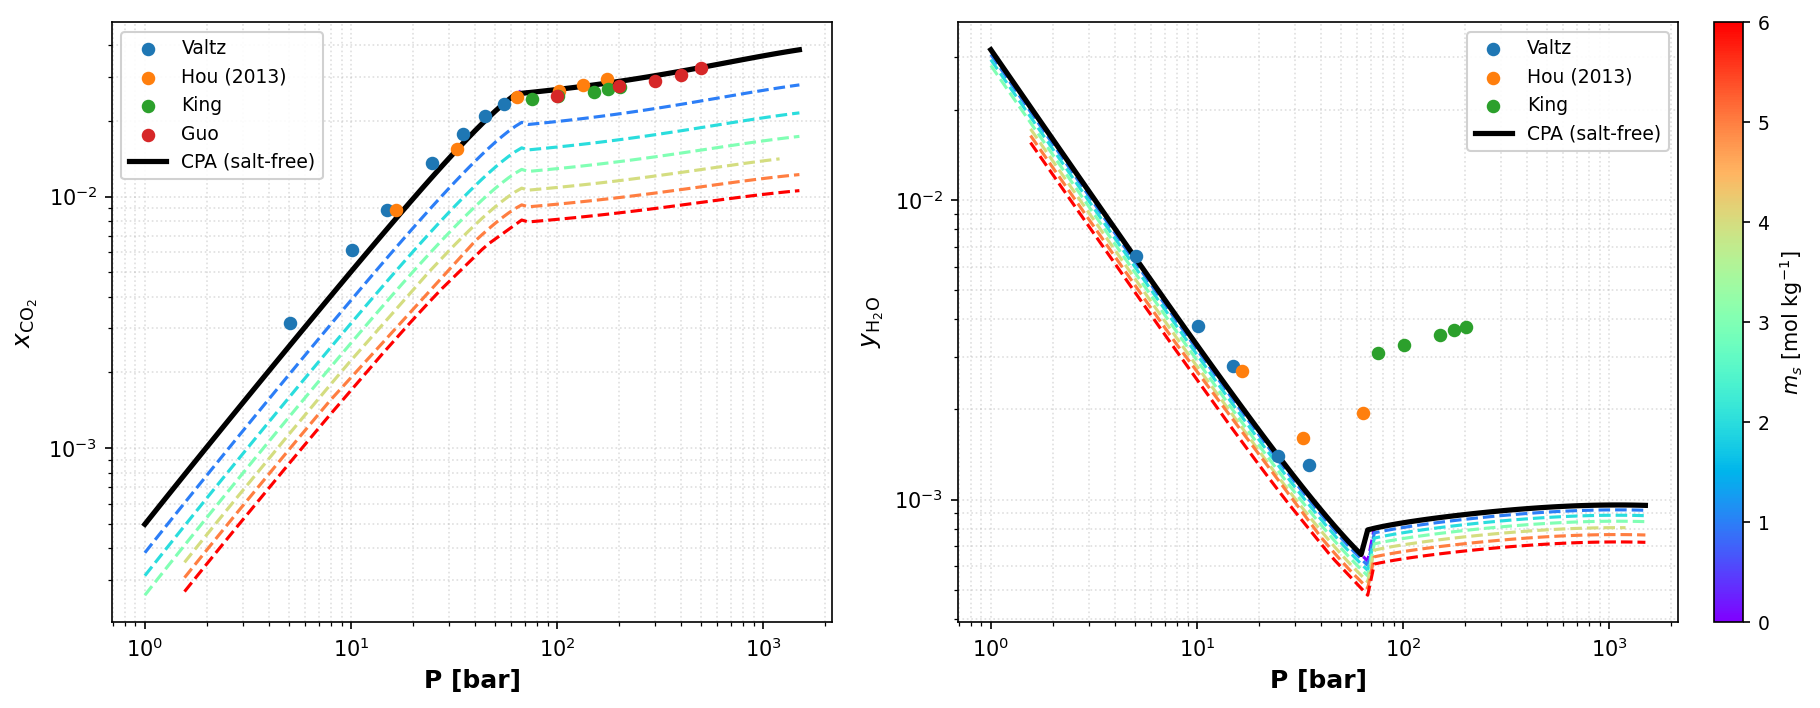
\includegraphics[width=\textwidth]{../figures/co2h2o/T298K.png}\caption{298\,K}\end{subfigure}\hfill
  \begin{subfigure}[t]{\sw}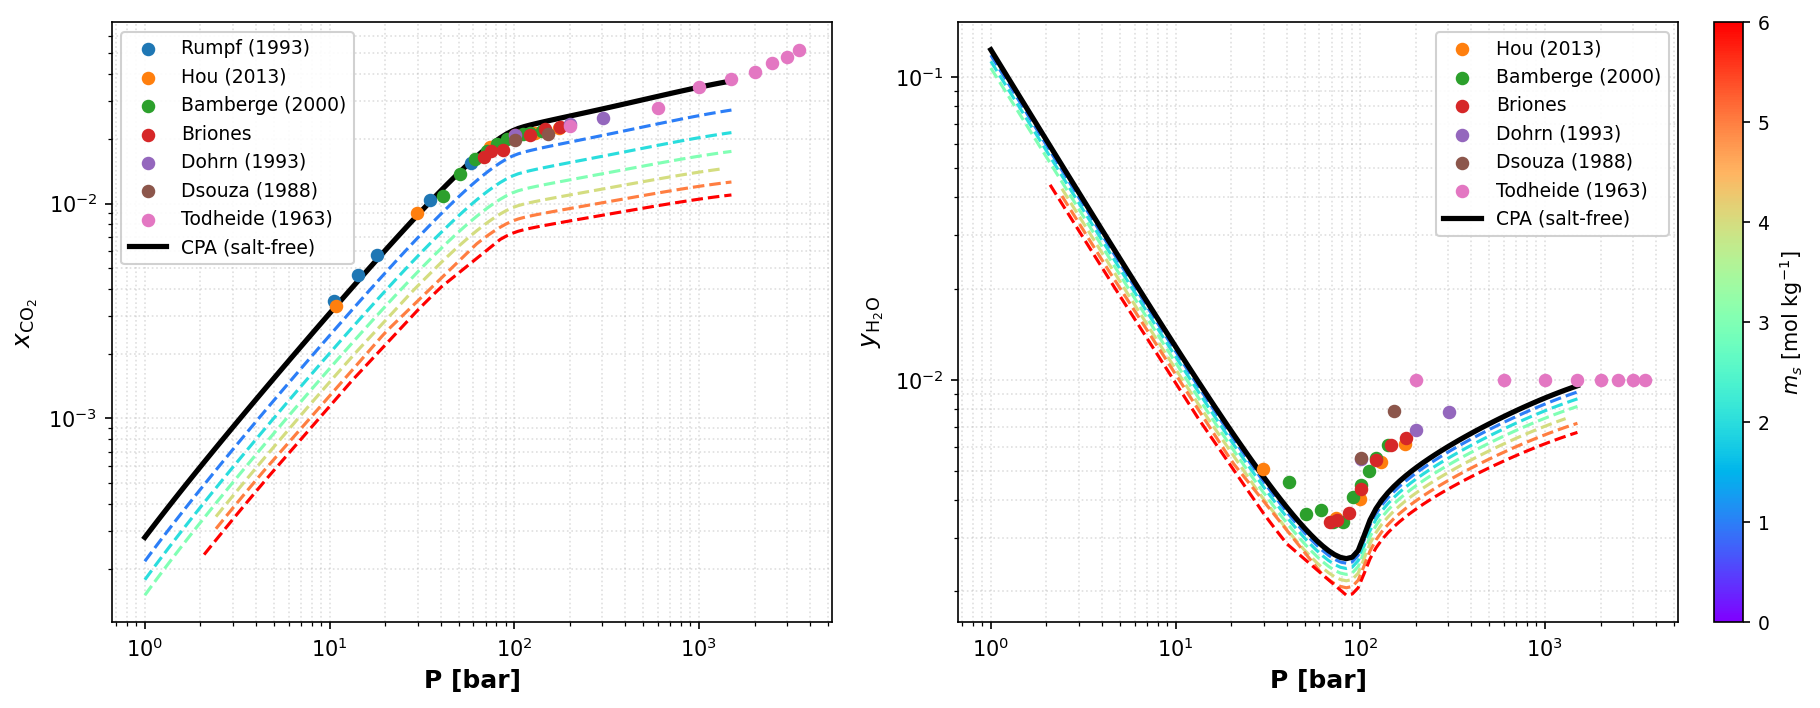
\includegraphics[width=\textwidth]{../figures/co2h2o/T323K.png}\caption{323\,K}\end{subfigure}\\[6pt]
  \begin{subfigure}[t]{\sw}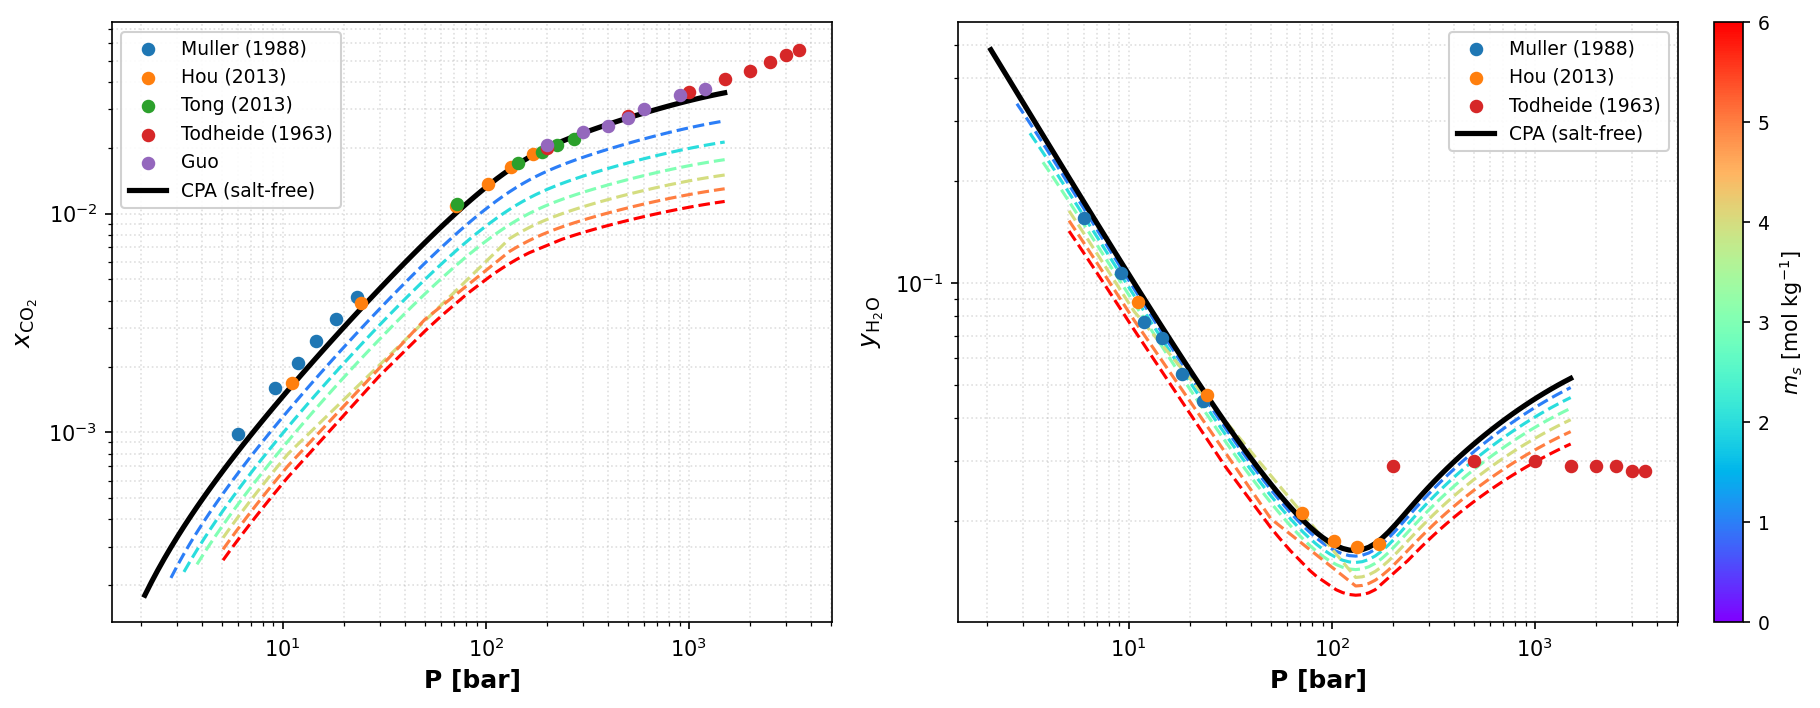
\includegraphics[width=\textwidth]{../figures/co2h2o/T373K.png}\caption{373\,K}\end{subfigure}\hfill
  \begin{subfigure}[t]{\sw}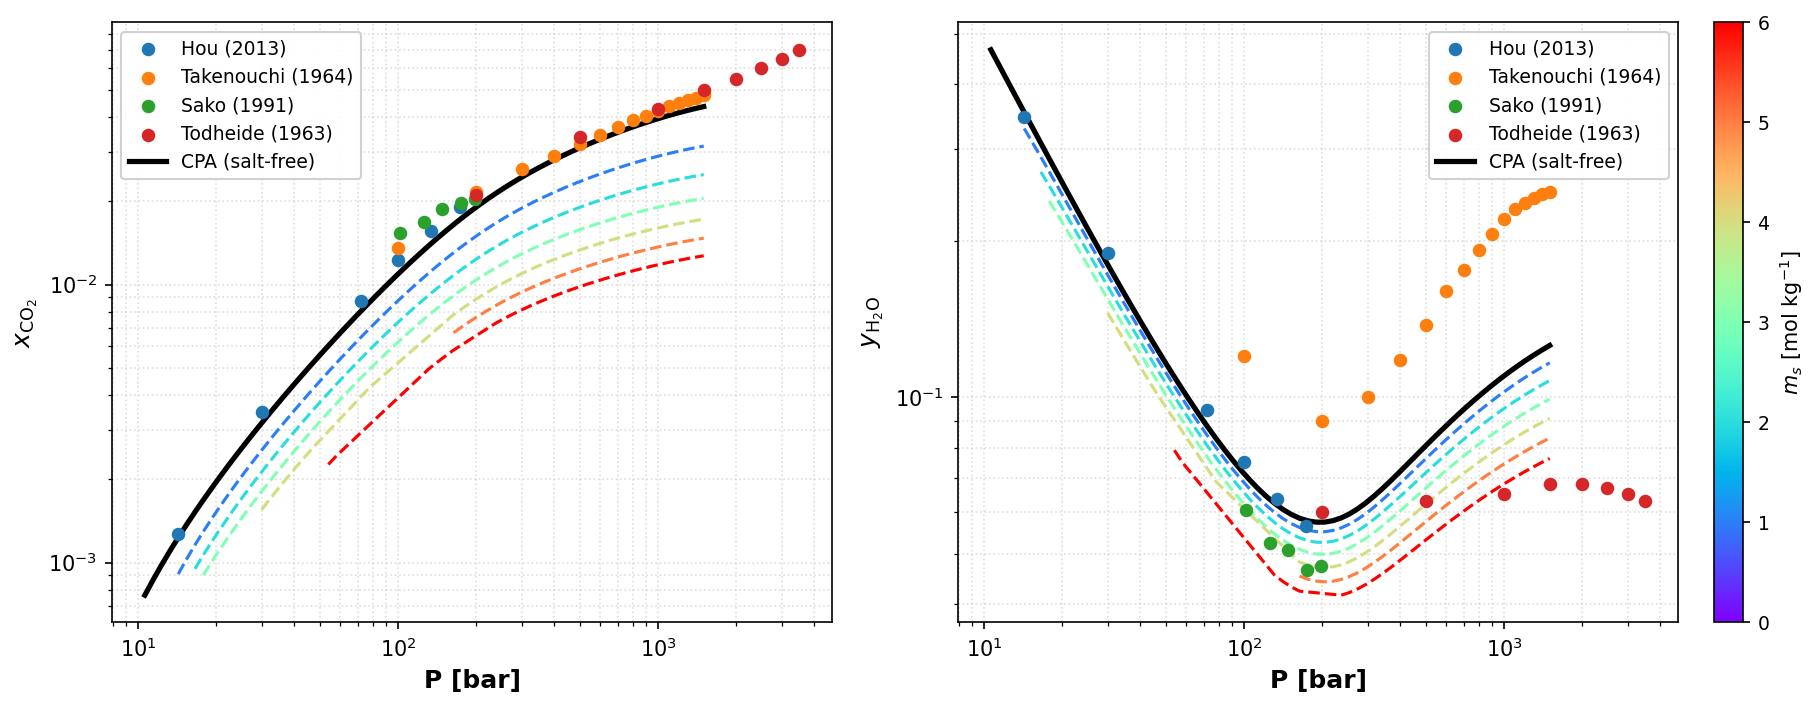
\includegraphics[width=\textwidth]{../figures/co2h2o/T423K.png}\caption{423\,K}\end{subfigure}\\[6pt]
  \begin{subfigure}[t]{\sw}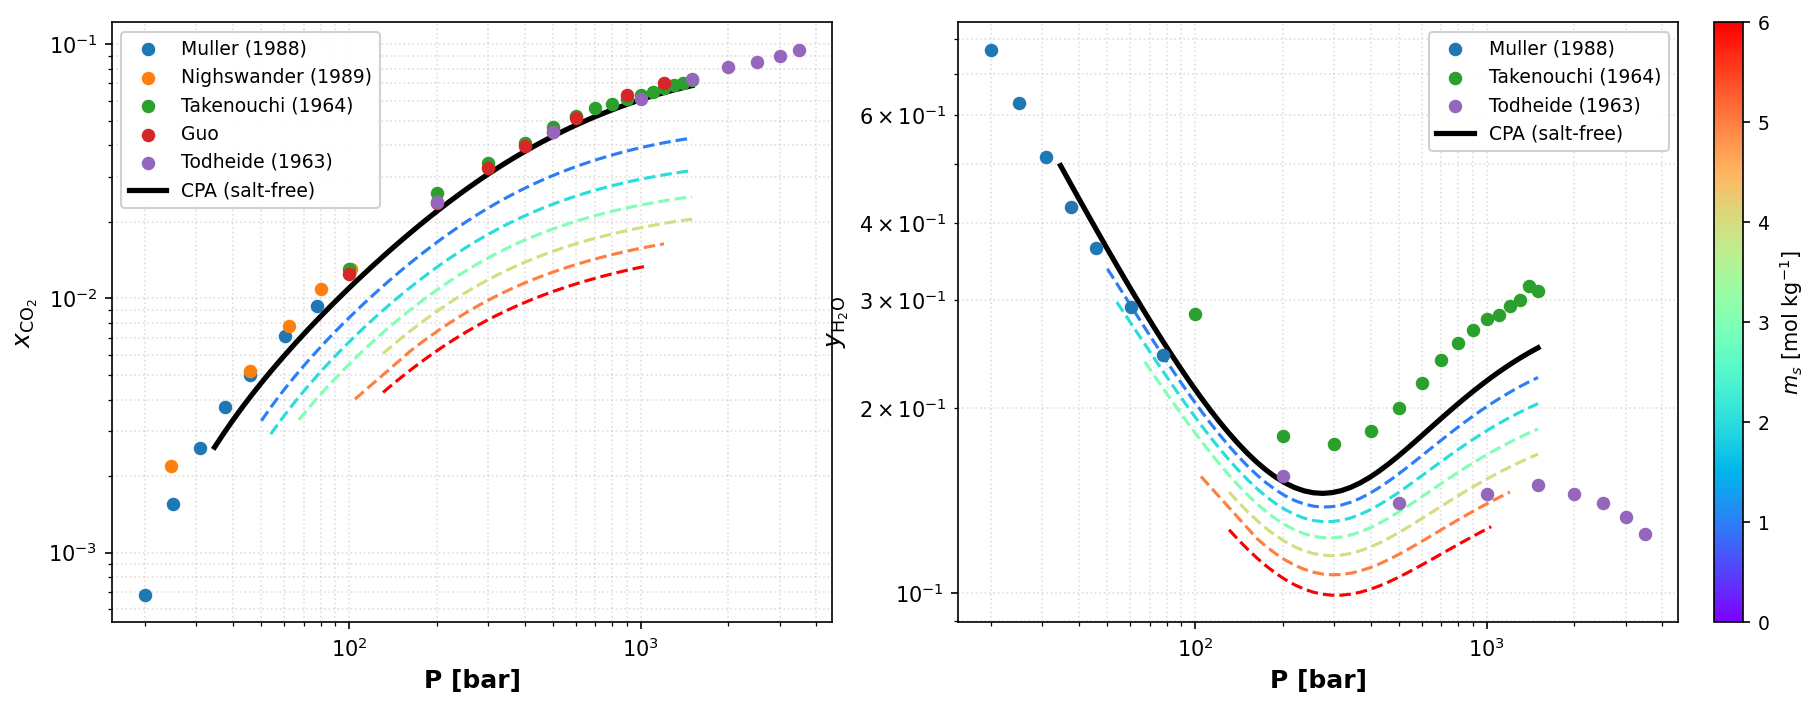
\includegraphics[width=\textwidth]{../figures/co2h2o/T473K.png}\caption{473\,K}\end{subfigure}\hfill
  \begin{subfigure}[t]{\sw}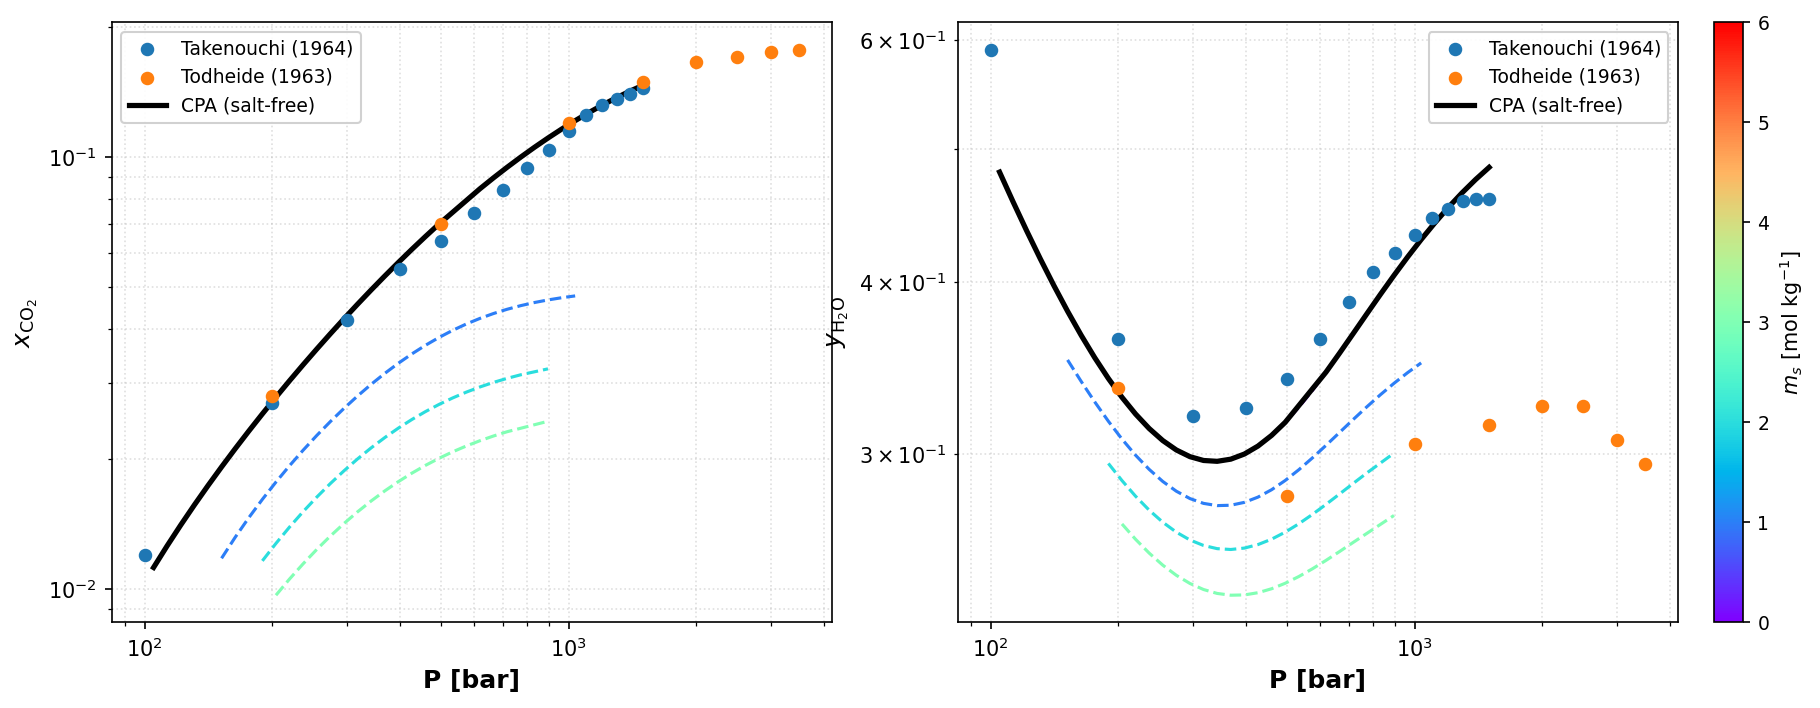
\includegraphics[width=\textwidth]{../figures/co2h2o/T523K.png}\caption{523\,K}\end{subfigure}
  \caption{CO$_2$ + H$_2$O phase equilibria at six representative temperatures (298--523\,K).
           For each temperature, the left panel shows the CO$_2$ mole fraction in the aqueous
           phase ($x_{\text{CO}_2}$) and the right panel shows the H$_2$O mole fraction in the
           CO$_2$-rich phase ($y_{\text{H}_2\text{O}}$) vs.\ pressure.
           Open symbols: experimental data \citep{Coelho2025}; black solid line: CPA (salt-free);
           dashed lines: eCPA predictions at NaCl molalities $m_s = 0$--$6$\,mol\,kg$^{-1}$
           (rainbow color scale; colorbar at right of each panel, violet = 0, red = 6\,mol\,kg$^{-1}$).
           Results for all 35 temperatures are shown in Fig.~\ref{fig:co2h2o_Tpanel_SI}.}
  \label{fig:co2h2o_Tpanel}
\end{figure}

\begin{figure}[h!]
  \centering
  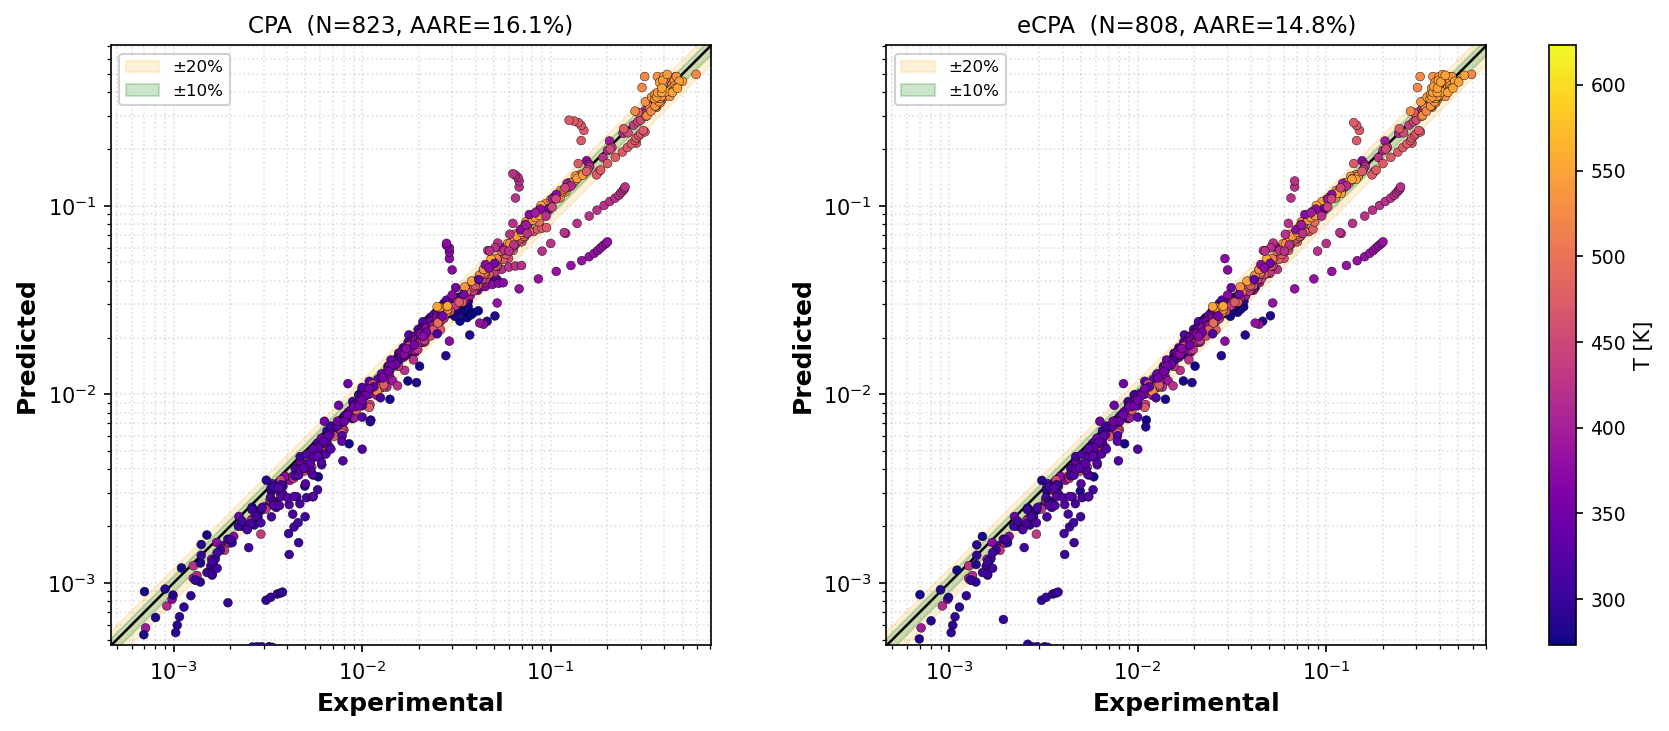
\includegraphics[width=0.85\textwidth]{../figures/validation_parity.png}
  \caption{Parity plots for the CO$_2$ + H$_2$O binary: CPA (left) and eCPA (right).
           Green and orange bands indicate $\pm 10\%$ and $\pm 20\%$ error, respectively.
           Points are colored by temperature.}
  \label{fig:co2h2o_parity}
\end{figure}

\subsection{CO$_2$ + NaCl brine}
\label{sec:co2nacl}

Figure~\ref{fig:co2h2o_Tpanel} also illustrates the effect of brine salinity on the equilibrium compositions by including predictions for the full molality range considered in this work. 
We further validate the eCPA ternary flash against all available experimental data from the
literature \citep{Guo2015, Rumpf1994, Koschel2006, Kiepe2002, Takenouchi1965,
Chabab2020, Messabeb2016, Hou2013, Yan2011, Zhao2015},
spanning $T = 278$--$723$\,K, $P = 1$--$1400$\,bar, and
$m_s = 0.17$--$6.0$\,mol\,kg$^{-1}$ NaCl (708 data points in total).
Three types of measurements are compared: CO$_2$ molality in the aqueous phase
($m_c$ [mol\,kg$^{-1}$]), the salt-free CO$_2$ mole fraction
($x_{\text{CO}_2}^{\text{sf}} = x_{\text{CO}_2}/(x_{\text{CO}_2}+x_{\text{H}_2\text{O}})$),
and the CO$_2$ mole fraction in the CO$_2$-rich phase ($y_{\text{CO}_2}$).

Table~\ref{tab:co2nacl_metrics} shows the accuracy breakdown by quantity type.
603 of 708 points converge to a two-phase solution; the remaining 105 are classified as
single-phase (particularly at $T \geq 623$\,K where CO$_2$ + H$_2$O approaches complete
miscibility) or fail to converge at extreme high-$P$, high-$m_s$ conditions.
Overall AARE across all converged points is 6.7\%, with a slight underprediction bias
of $-1.0\%$.
The AARE for $m_c$ across all $T$ and $m_s$ is 6.9\%, consistent with the 6.9\%
reported by \citet{Coelho2025}.
The CO$_2$-rich phase composition $y_{\text{CO}_2}$ is reproduced to within 0.4\% AARE, reflecting the
near-purity of the CO$_2$-rich phase and its weak dependence on salinity.

At hydrothermal temperatures ($T = 573$--$623$\,K), AARE for $m_c$ rises to 14.0\% and
12.8\%, respectively, reflecting reduced eCPA accuracy at conditions beyond the
conventional reservoir temperature range.
At $T \geq 673$\,K, the available experimental pressures (300--900\,bar, all from
\citealt{Takenouchi1965}) fall in the region where eCPA predicts single-phase behavior,
suggesting that the CO$_2$ + H$_2$O miscibility gap closes at these extreme conditions
in the model.
Notably, accuracy at the lowest temperatures ($T = 278$--$283$\,K) is also reduced
(AARE 14--21\%), reflecting the challenge of modeling CO$_2$ solubility very close to
the freezing point where eCPA is not specifically parameterized.
Figure~\ref{fig:co2nacl_heatmap} provides a comprehensive view of the error distribution
across the full $(T, m_s)$ parameter space: accuracy is best at intermediate temperatures
($T = 300$--$500$\,K) and moderate salinities ($m_s \leq 3$\,mol\,kg$^{-1}$), and degrades
systematically at the boundaries of the validated range.

\begin{table}[htb]
  \centering
  \caption{VLE accuracy metrics for CO$_2$ + NaCl brine ($T = 278$--$723$\,K,
           $m_s = 0.17$--$6.0$\,mol\,kg$^{-1}$, 708 data points total,
           603 converged). Bias $= \langle(\hat{y} - y)/y\rangle$.}
  \label{tab:co2nacl_metrics}
  \begin{tabular}{lrrr}
    \toprule
    Quantity & $N$ & AARE (\%) & Bias (\%) \\
    \midrule
    $m_c$ [mol\,kg$^{-1}$] & 440 & 6.9 & $-3.1$ \\
    $x_{\text{CO}_2}^{\text{sf}}$     & 99  & 7.0 & $+4.3$ \\
    $x_{\text{CO}_2}$ [salt-incl.]    & 36  & 8.5 & $+8.5$ \\
    $y_{\text{CO}_2}$                 & 28  & 0.4 & $-0.0$ \\
    \midrule
    All converged           & 603 & 6.7 & $-1.0$ \\
    \bottomrule
  \end{tabular}
\end{table}

\begin{figure}[h!]
  \centering
  \newcommand{\snw}{0.30\textwidth}%
  \begin{subfigure}[t]{\snw}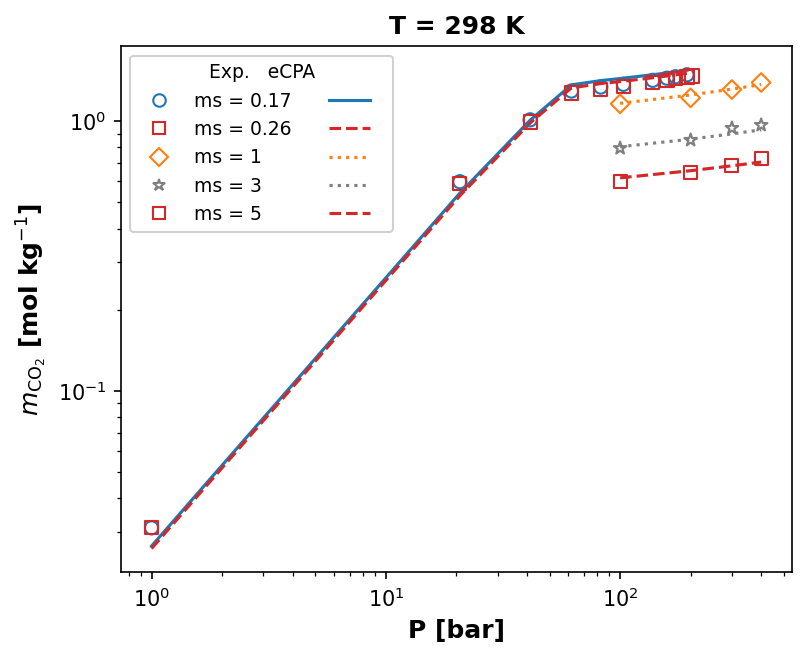
\includegraphics[width=\textwidth]{../figures/co2nacl/T298K.png}\caption{298\,K}\end{subfigure}\hfill
  \begin{subfigure}[t]{\snw}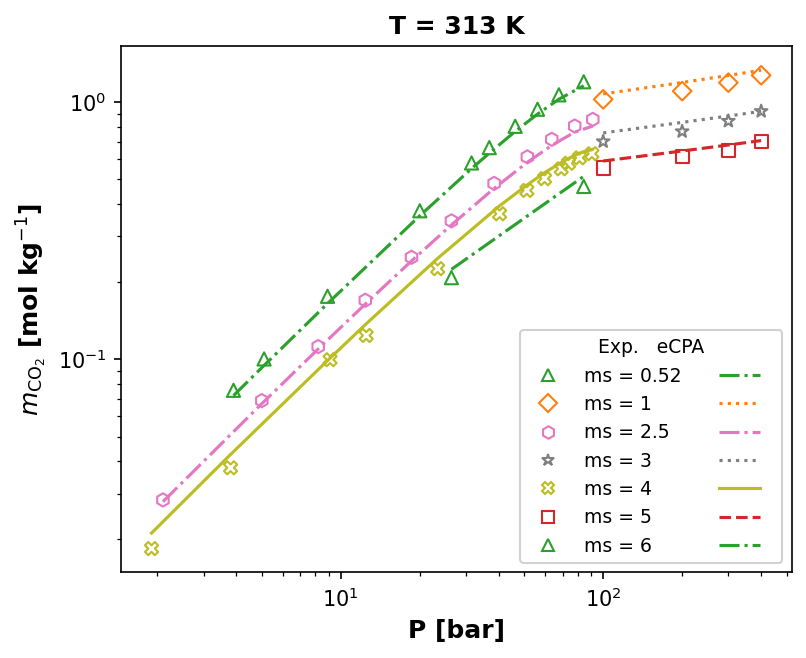
\includegraphics[width=\textwidth]{../figures/co2nacl/T313K.png}\caption{313\,K}\end{subfigure}\hfill
  \begin{subfigure}[t]{\snw}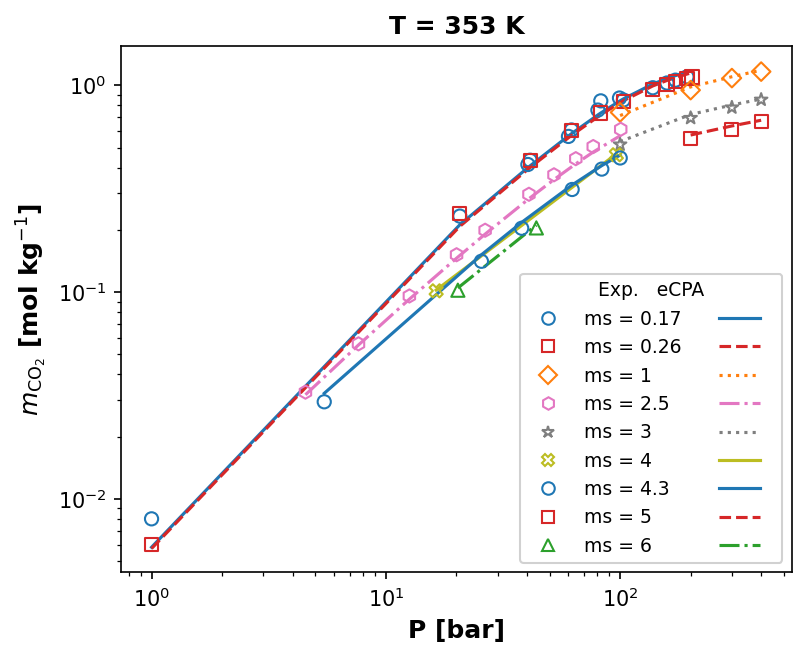
\includegraphics[width=\textwidth]{../figures/co2nacl/T353K.png}\caption{353\,K}\end{subfigure}\\[6pt]
  \begin{subfigure}[t]{\snw}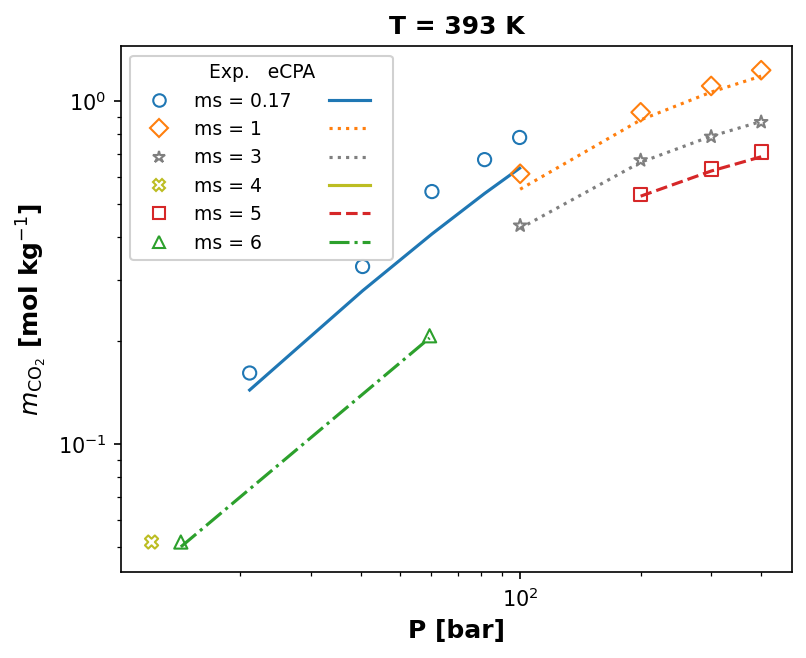
\includegraphics[width=\textwidth]{../figures/co2nacl/T393K.png}\caption{393\,K}\end{subfigure}\hfill
  \begin{subfigure}[t]{\snw}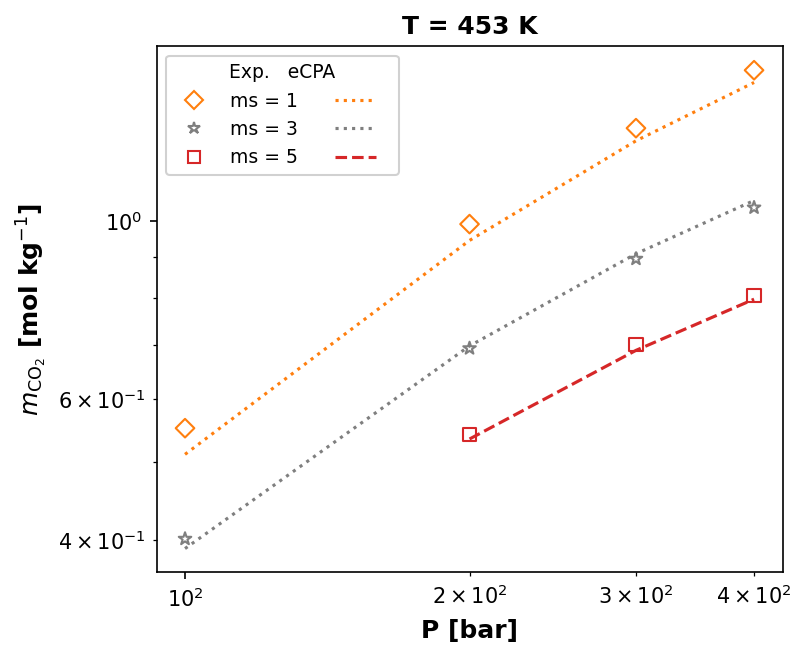
\includegraphics[width=\textwidth]{../figures/co2nacl/T453K.png}\caption{453\,K}\end{subfigure}\hfill
  \begin{subfigure}[t]{\snw}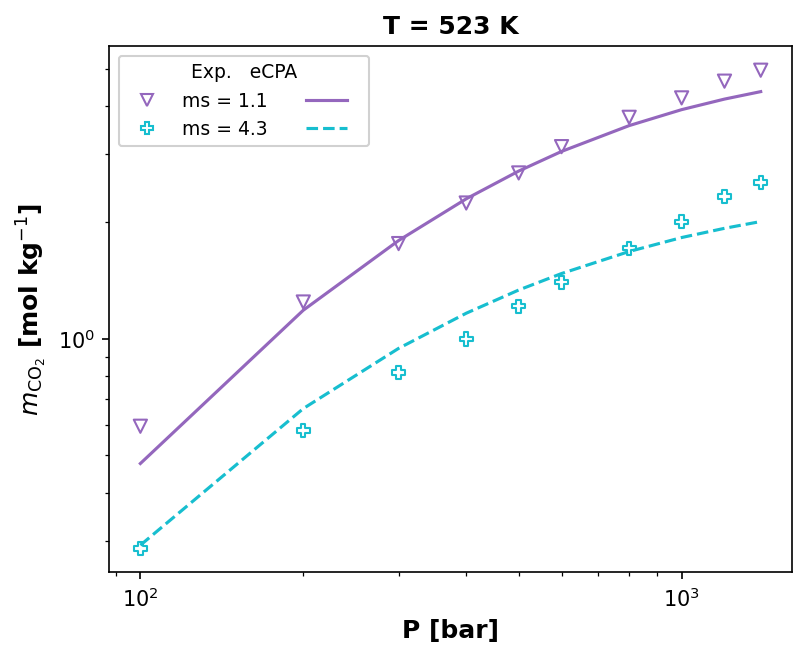
\includegraphics[width=\textwidth]{../figures/co2nacl/T523K.png}\caption{523\,K}\end{subfigure}
  \caption{CO$_2$ solubility in NaCl brine at six representative temperatures (298--523\,K).
           Each panel shows CO$_2$ molality $m_c$ [mol\,kg$^{-1}$] vs.\ pressure (log--log).
           Open symbols: experimental data; lines: eCPA.
           Colors and markers distinguish NaCl molalities (see legend).
           Temperatures with additional CO$_2$-rich phase data ($y_{\text{CO}_2}$) are shown separately
           in Fig.~\ref{fig:co2nacl_2panel}; all 18 temperatures in Fig.~\ref{fig:co2nacl_Tpanel_SI}.}
  \label{fig:co2nacl_Tpanel}
\end{figure}

\begin{figure}[h!]
  \centering
  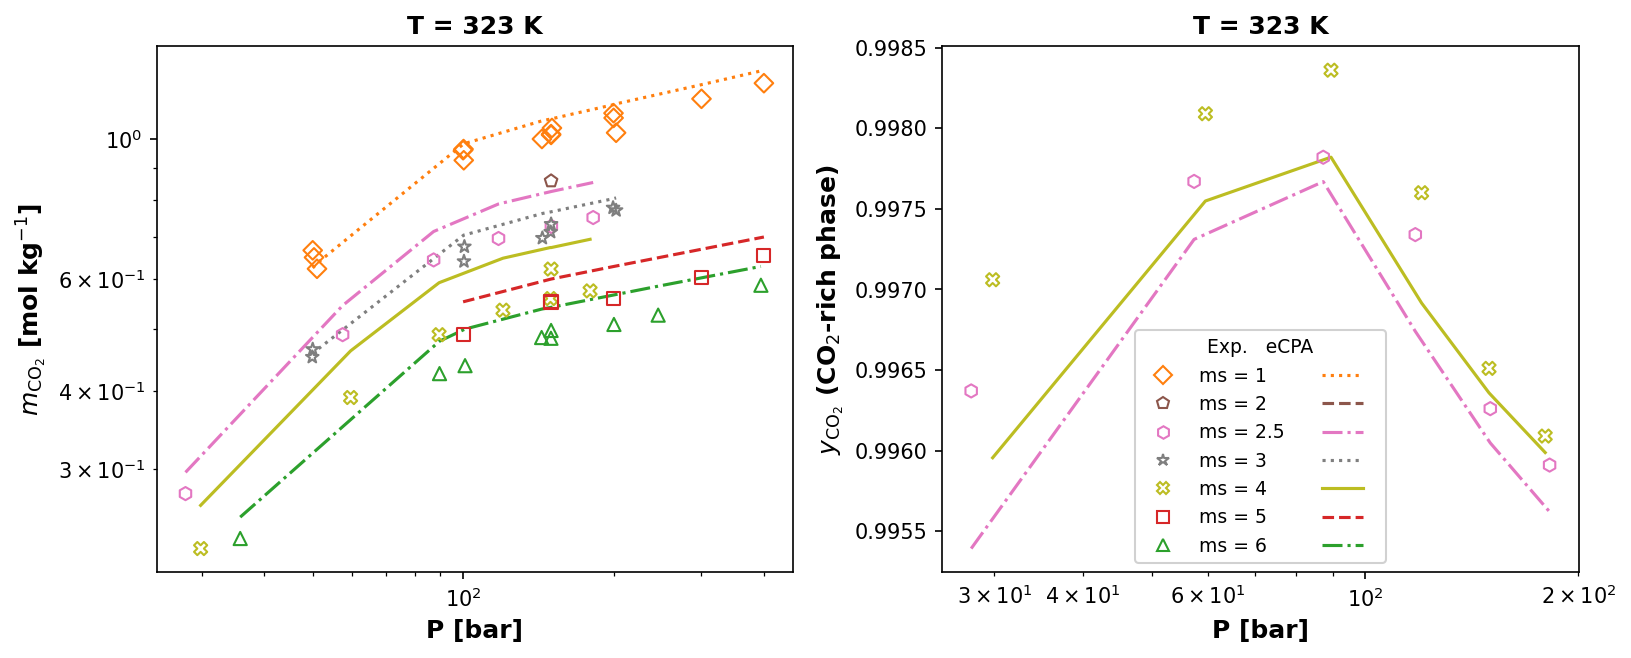
\includegraphics[width=0.88\textwidth]{../figures/co2nacl/T323K.png}\\[6pt]
  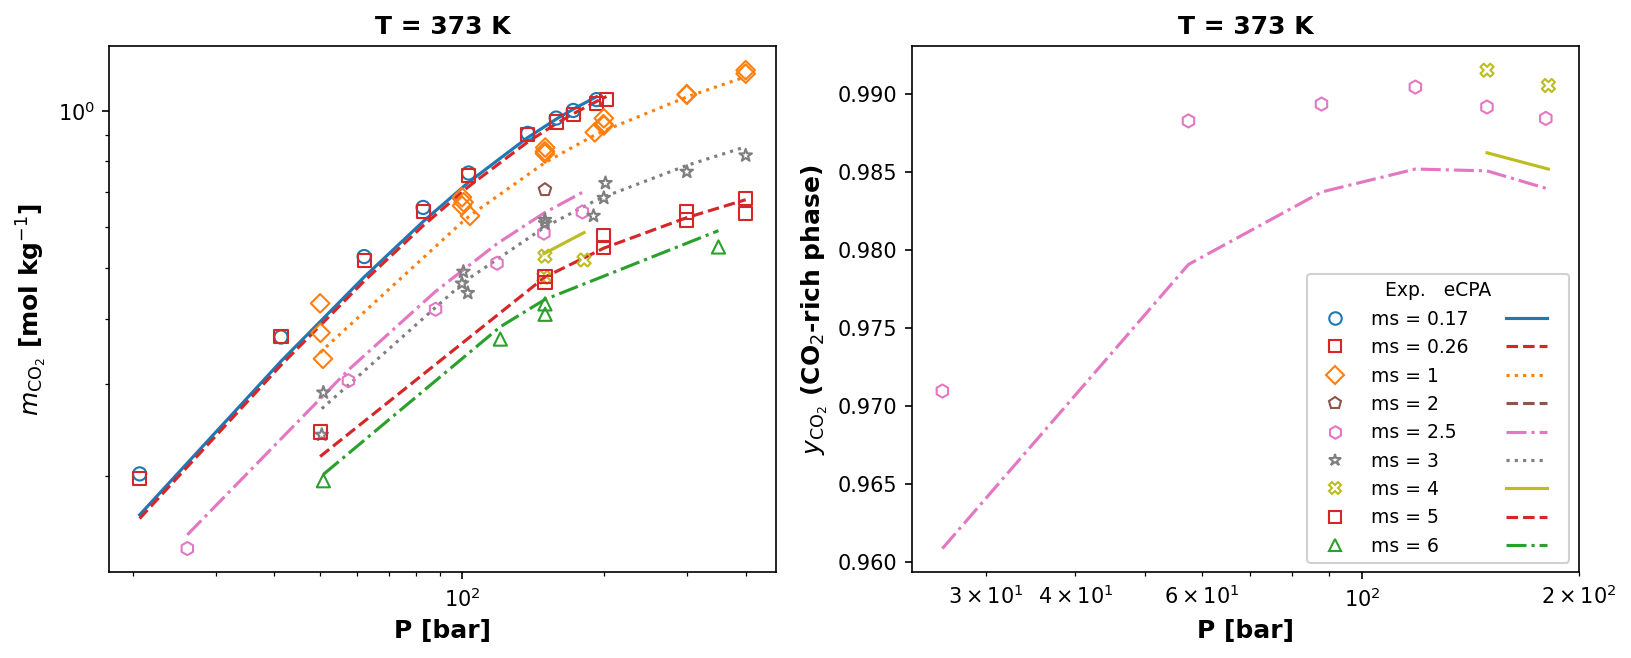
\includegraphics[width=0.88\textwidth]{../figures/co2nacl/T373K.png}\\[6pt]
  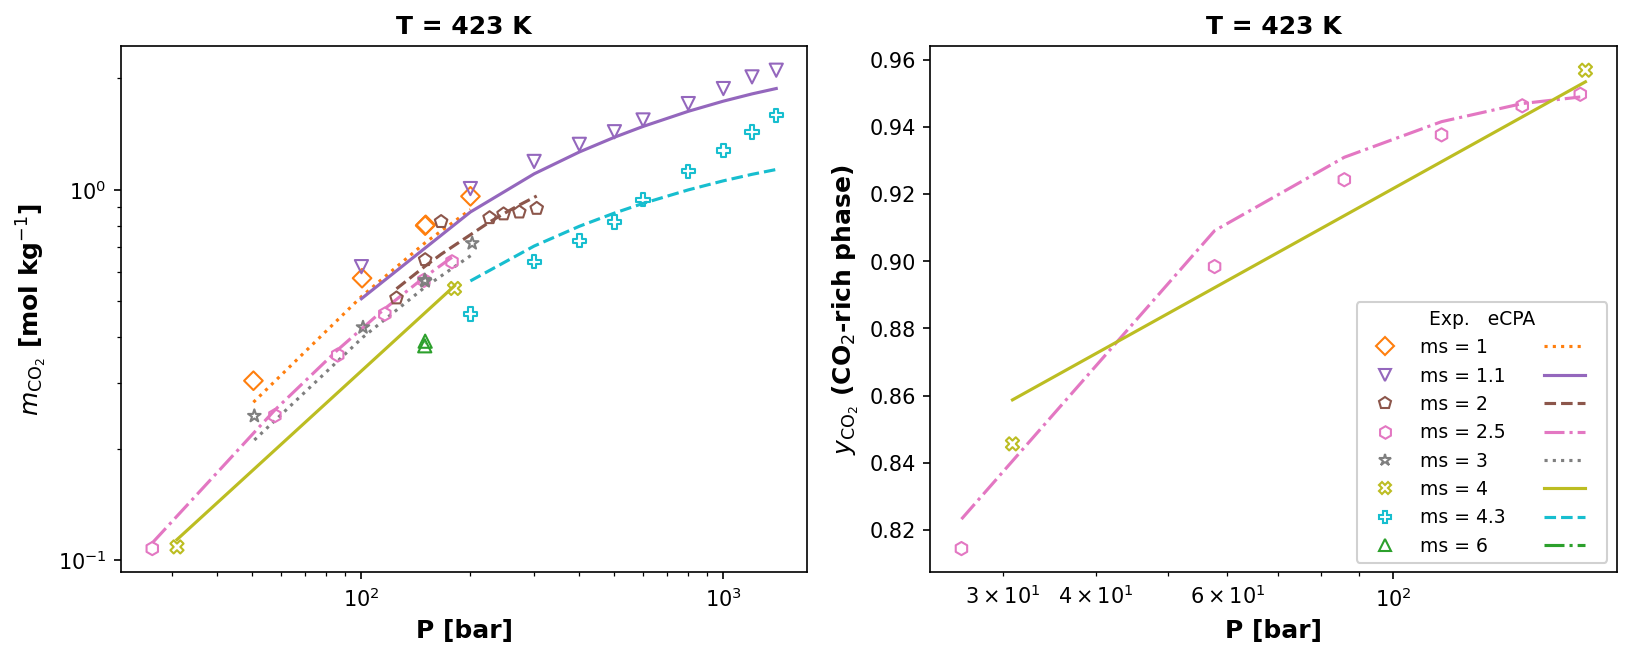
\includegraphics[width=0.88\textwidth]{../figures/co2nacl/T423K.png}
  \caption{CO$_2$ + NaCl brine phase equilibria at temperatures for which both CO$_2$ molality
           ($m_c$, left panel) and CO$_2$ mole fraction in the CO$_2$-rich phase ($y_{\text{CO}_2}$, right panel)
           data are available: (top) 323\,K, (middle) 373\,K, (bottom) 423\,K.
           Open symbols: experimental data; lines: eCPA.
           Colors and markers distinguish NaCl molalities (see legend).}
  \label{fig:co2nacl_2panel}
\end{figure}

\begin{figure}[h!]
  \centering
  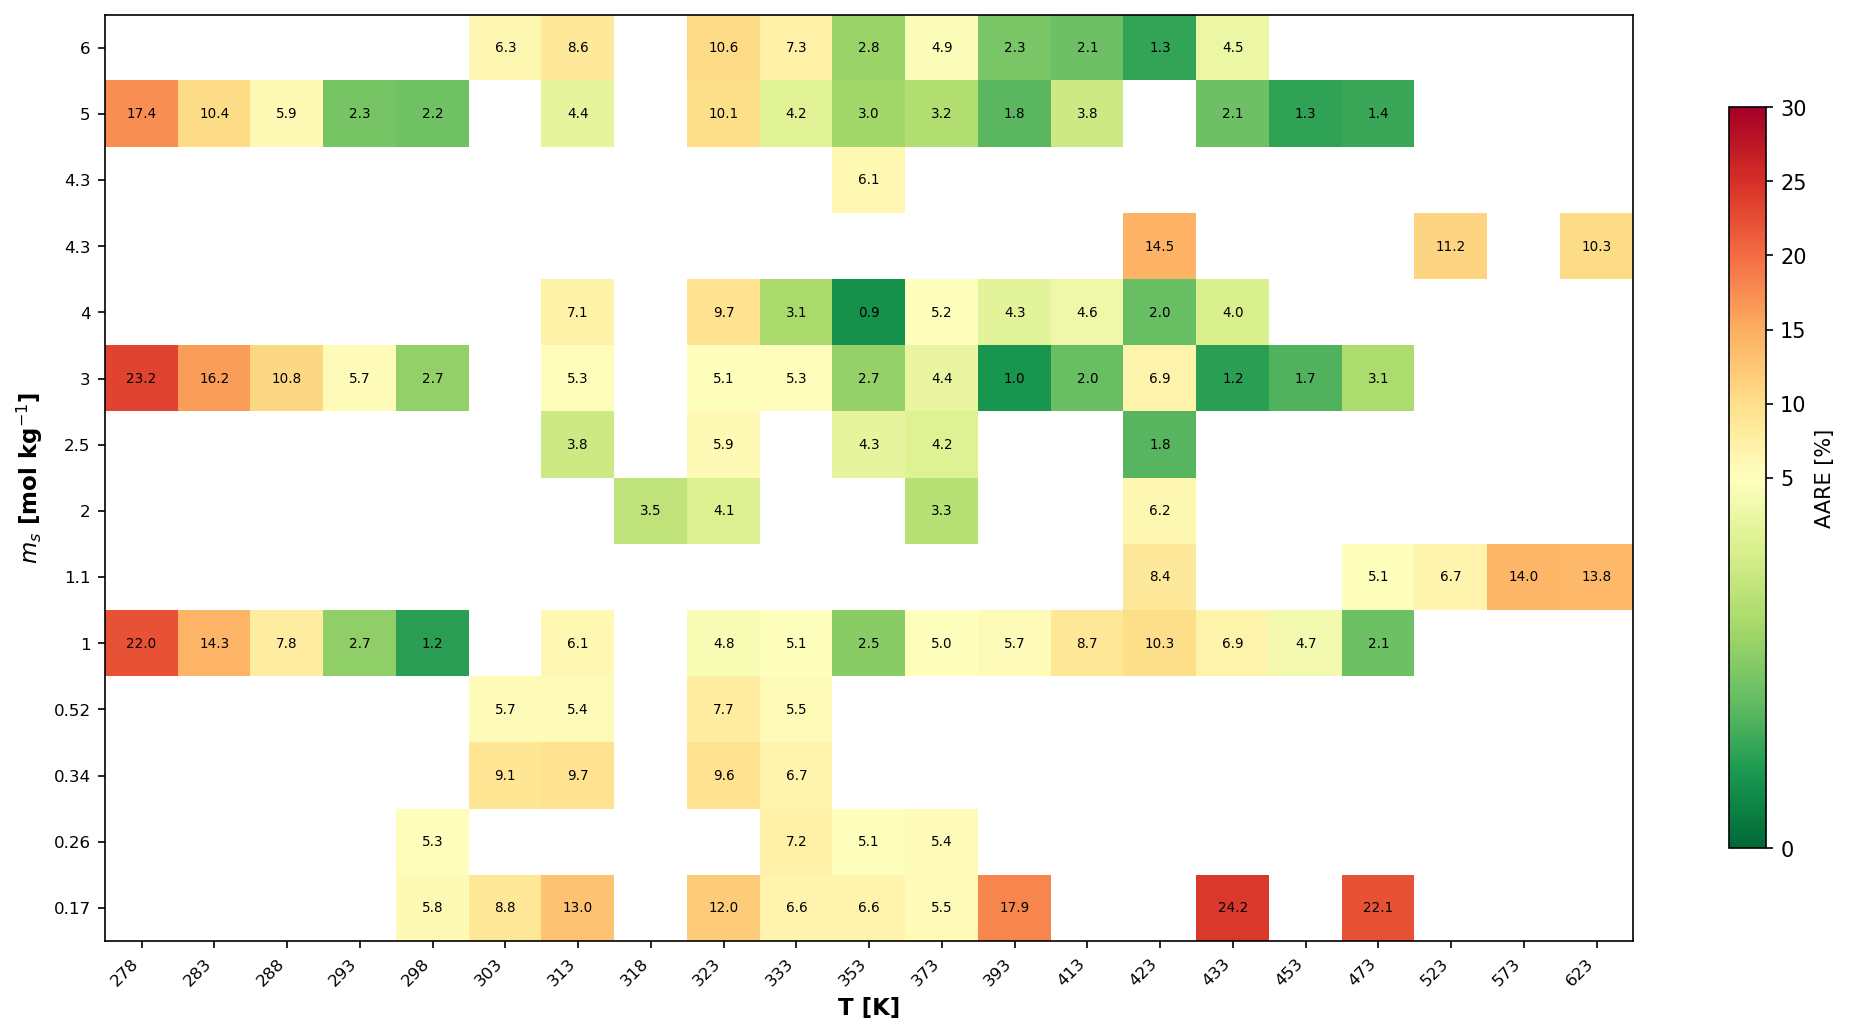
\includegraphics[width=0.85\textwidth]{../figures/validation_heatmap_extended.png}
  \caption{Heatmap of absolute relative error (AARE, \%) for the CO$_2$ + NaCl
           validation dataset ($T = 278$--$623$\,K), showing all individual NaCl
           molalities present in the experimental data.
           Color scale is diverging at 5\%: green $\leq 5\%$, red $\geq 10\%$.
           Empty cells indicate no experimental data at that $(T, m_s)$ combination.}
  \label{fig:co2nacl_heatmap}
\end{figure}

\subsection{Flash results as a function of feed composition}
\label{sec:flash_vs_z}

A central motivation for full stability+flash --- rather than straightforward
VLE calculations at a fixed salinity --- arises naturally in reservoir simulation.
When CO$_2$ is injected into a saline aquifer, the reservoir fluid at any given
grid cell can be represented as a mixture of brine (carrying NaCl at feed molality
$m_\mathrm{feed}$) and varying amounts of injected CO$_2$.
The overall CO$_2$ mole fraction $z$ in this mixture is the primary degree of freedom,
and stability+flash must be performed to determine the equilibrium state.

A subtlety that distinguishes the full flash from simple VLE lookup is that, as
$z$ increases inside the two-phase window, more H$_2$O partitions into the growing
CO$_2$-rich phase.
The amount of water remaining in the aqueous phase therefore decreases, while the
NaCl inventory is fixed --- causing the \emph{equilibrium} aqueous molality
$m_s^\mathrm{aq}$ to \emph{exceed} the feed molality $m_\mathrm{feed}$.
This salting-out feedback reduces CO$_2$ solubility and in turn changes the
CO$_2$-phase water content, so that equilibrium phase compositions are
\emph{not} independent of $z$ once the NaCl molality is defined on a feed basis.

Figure~\ref{fig:flash_vs_z} demonstrates these effects for $P = 200$\,bar,
$m_\mathrm{feed} = 1.0$\,mol\,kg$^{-1}$ NaCl, and four temperatures
(350, 400, 450, 500\,K) over the two-phase feed range $z = 0.01$--$0.99$.
Panel (a) shows the CO$_2$-rich phase fraction $\beta$, which rises from 0 to 1
across the two-phase window.
Higher temperatures narrow the window because CO$_2$ is less soluble and
H$_2$O more volatile, both effects shrinking the range of $z$ that sustains
two-phase coexistence.

Panel (b) illustrates the salinity amplification: at $T = 500$\,K the ratio
$m_s^\mathrm{aq}/m_\mathrm{feed}$ reaches 2.2 at the high-$z$ end of the
two-phase window, meaning the aqueous NaCl concentration more than doubles
relative to the injected brine.
At lower temperatures the amplification is smaller because less H$_2$O leaves
the aqueous phase at the lower $\beta$ values attained.

Panel (c) shows the resulting CO$_2$ molality in the aqueous phase,
$m_c$ [mol\,kg$^{-1}$].
Despite operating at fixed $(T, P)$, $m_c$ decreases noticeably with increasing
$z$: at $T = 500$\,K it falls from $\approx 1.1$ to $\approx 0.9$\,mol\,kg$^{-1}$
across the two-phase window.
This is a direct consequence of the salting-out effect --- the elevated
$m_s^\mathrm{aq}$ suppresses CO$_2$ solubility.
A simple VLE lookup at the feed molality $m_\mathrm{feed}$ would return the
wrong CO$_2$ solubility for all but the dilute-CO$_2$ end of the window.

Panel (d) shows the H$_2$O mole fraction in the CO$_2$-rich phase $y_{\text{H}_2\text{O}}$,
which likewise varies with $z$ (and hence with $m_s^\mathrm{aq}$) and increases
strongly with temperature.
At $T = 500$\,K, up to $\approx 23$\,mol\% of the CO$_2$-rich phase is water,
underscoring the importance of accurate modeling of this phase at high temperatures.

Taken together, these results demonstrate that the correct representation of
CO$_2$+brine phase behavior in reservoir models requires a full
stability+flash computation for each cell at each time step, with the
NaCl molality updated self-consistently from the aqueous-phase amount.

\begin{figure}[h!]
  \centering
  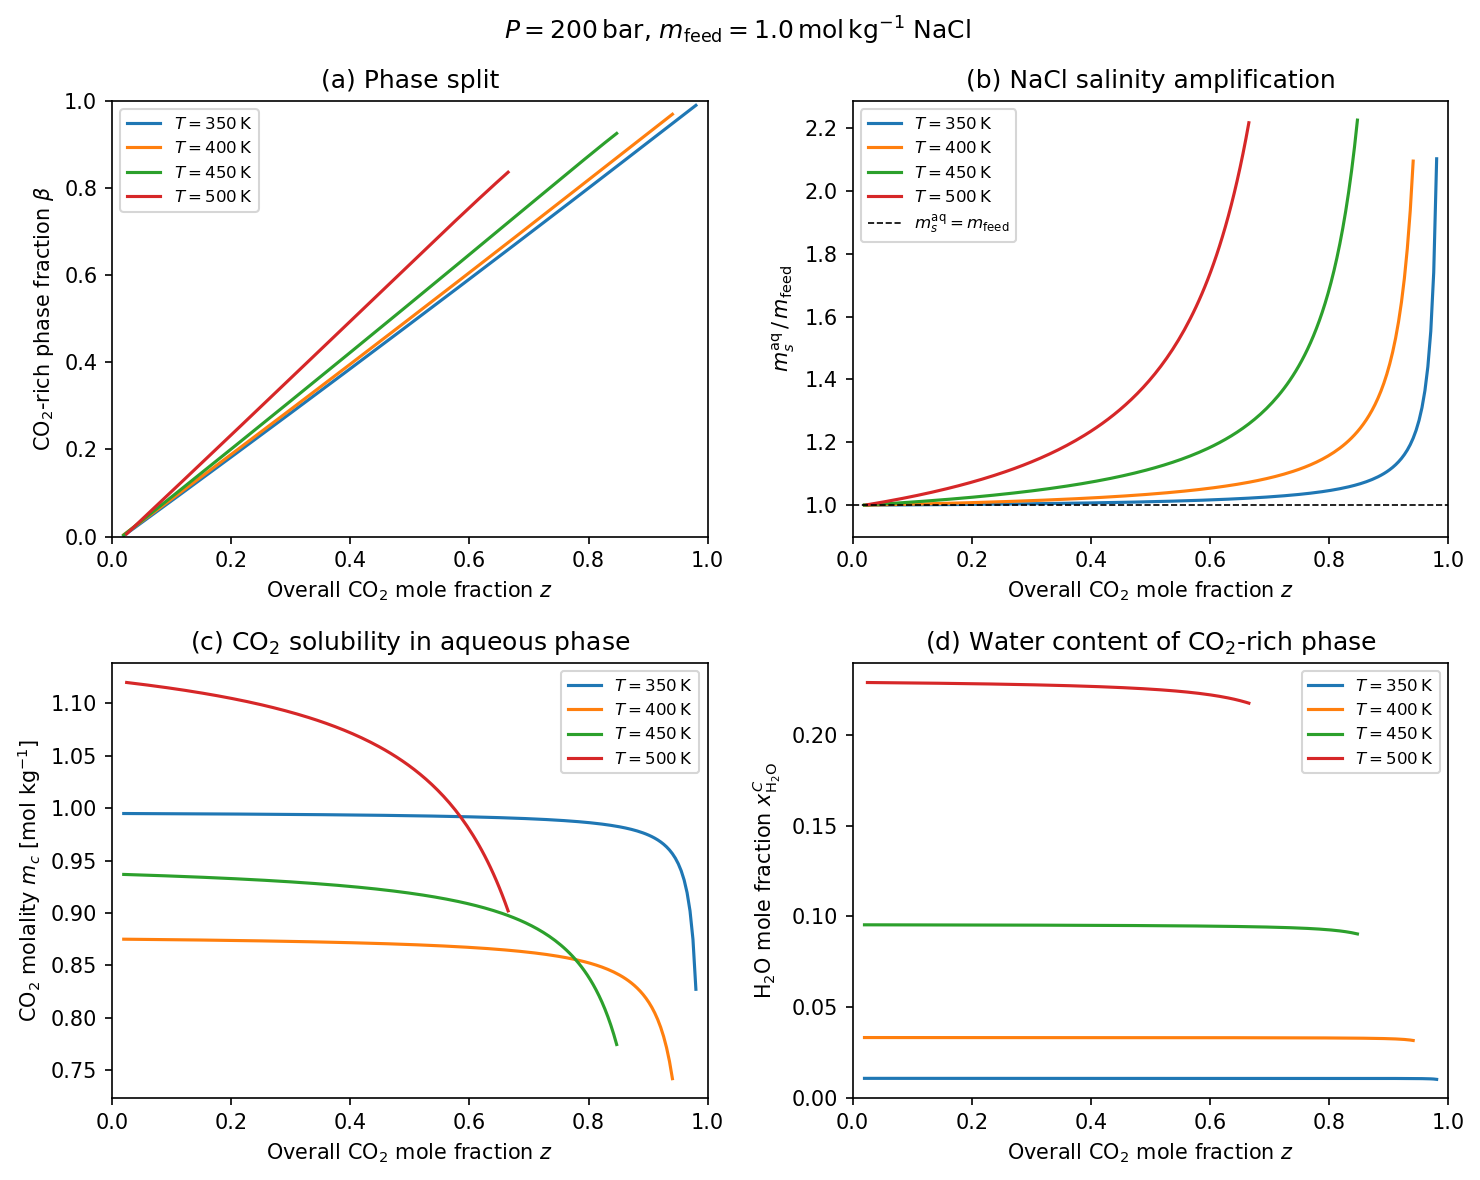
\includegraphics[width=\textwidth]{../figures/flash_vs_z.png}
  \caption{eCPA flash results as a function of overall CO$_2$ feed mole fraction $z$
           at $P = 200$\,bar, feed molality $m_\mathrm{feed} = 1.0$\,mol\,kg$^{-1}$
           NaCl, and four temperatures (350, 400, 450, 500\,K).
           (a) CO$_2$-rich phase fraction $\beta$; the two-phase window narrows at
           higher temperature.
           (b) Ratio of equilibrium aqueous NaCl molality to feed molality,
           $m_s^\mathrm{aq}/m_\mathrm{feed}$; NaCl concentrates in the aqueous phase
           as H$_2$O partitions to the CO$_2$-rich phase, reaching a factor of 2.2
           at $T = 500$\,K.
           (c) CO$_2$ molality $m_c$ in the aqueous phase; the salting-out effect
           driven by the elevated $m_s^\mathrm{aq}$ reduces CO$_2$ solubility
           with increasing $z$.
           (d) H$_2$O mole fraction in the CO$_2$-rich phase $y_{\text{H}_2\text{O}}$; substantial
           water content at high temperatures (up to 23\,mol\% at 500\,K) and its
           variation with $z$ highlight the need for full flash rather than
           a fixed-salinity VLE lookup.}
  \label{fig:flash_vs_z}
\end{figure}

\subsection{Aqueous-phase density}
\label{sec:density}

Aqueous-phase densities $\rho_W$ for CO$_2$-saturated water ($m_s = 0$) were compiled from
two experimental sources: \citet{King1992} (37 points, $T = 288$--$298$\,K) and
\citet{Nighswander1989} ($T = 353$--$473$\,K), for a total of 37 points at $T = 288$--$473$\,K.
In the two-phase region, phase compositions are independent of the overall CO$_2$ mole fraction,
so a fixed value $z_{\text{CO}_2} = 0.3$ was used for all flash calls; the eCPA density was
computed by directly solving the equilibrium equations at each $(T, P)$ using a Newton solver
(avoiding interpolation artefacts near the CO$_2$ critical region).

Without any volume shift (Péneloux $c_i = 0$), both CPA and eCPA overpredict aqueous density
by 0.76\% AARE with a systematic positive bias of the same magnitude, consistent with the
known tendency of SRK-based models to underpredict liquid molar volumes.

We optimize the H$_2$O Péneloux shift $c_{\text{H}_2\text{O}}$ by minimising AARE over the 37
data points using Brent's method.
The optimal shift is $c_{\text{H}_2\text{O}} = 0.1105$\,cm$^3$\,mol$^{-1}$ (Table~\ref{tab:peneloux}),
which reduces AARE from 0.76\% to \textbf{0.33\%} and nearly eliminates the systematic bias
($+0.19\%$).
This shift is an original contribution beyond \citet{Coelho2025}, who apply a volume correction
only to the NaCl component.

\begin{table}[htb]
  \centering
  \caption{Péneloux volume shifts used in this work.
           $c_s$ from \citet{Coelho2025}; $c_{\text{H}_2\text{O}}$ optimized here.}
  \label{tab:peneloux}
  \begin{tabular}{llcc}
    \toprule
    Species & Symbol & $c$ (cm$^3$\,mol$^{-1}$) & Source \\
    \midrule
    NaCl        & $c_s$              & $-53.5$ & \citet{Coelho2025} \\
    H$_2$O      & $c_{\text{H}_2\text{O}}$ & $+0.1105$ & This work \\
    CO$_2$      & $c_{\text{CO}_2}$  & $0$     & --- \\
    \bottomrule
  \end{tabular}
\end{table}

Figure~\ref{fig:density} compares experimental densities with CPA and eCPA predictions after
applying the optimized shift; the two models give essentially identical results at $m_s = 0$
because the electrostatic terms vanish in the absence of ions.

\begin{figure}[h!]
  \centering
  \begin{subfigure}[t]{0.32\textwidth}
    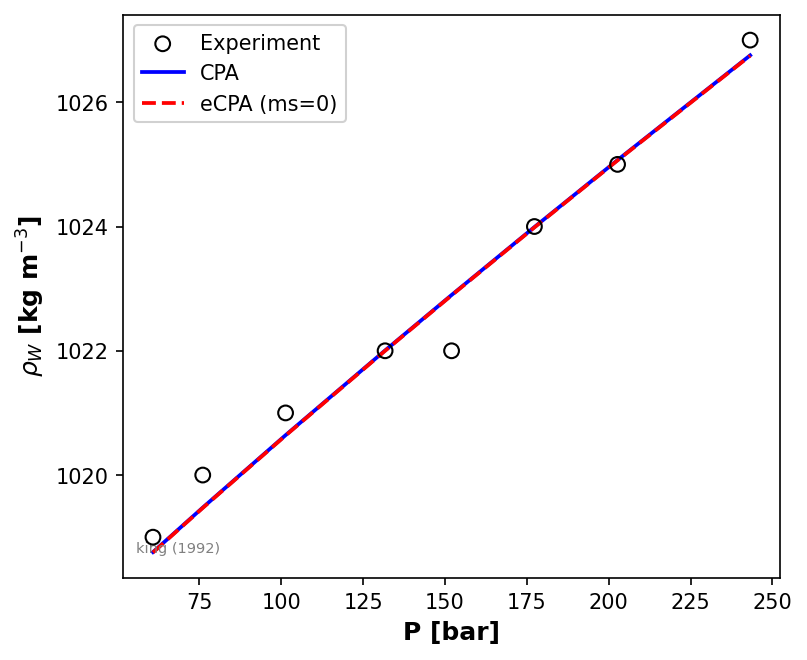
\includegraphics[width=\textwidth]{../figures/density/T288K.png}
    \caption{$T = 288$\,K}
  \end{subfigure}\hfill
  \begin{subfigure}[t]{0.32\textwidth}
    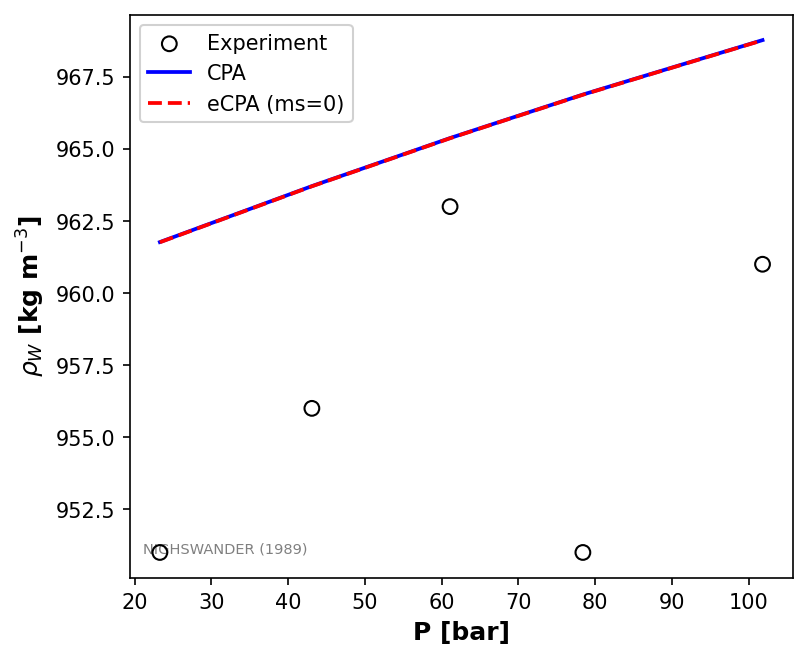
\includegraphics[width=\textwidth]{../figures/density/T353K.png}
    \caption{$T = 353$\,K}
  \end{subfigure}
  \begin{subfigure}[t]{0.32\textwidth}
    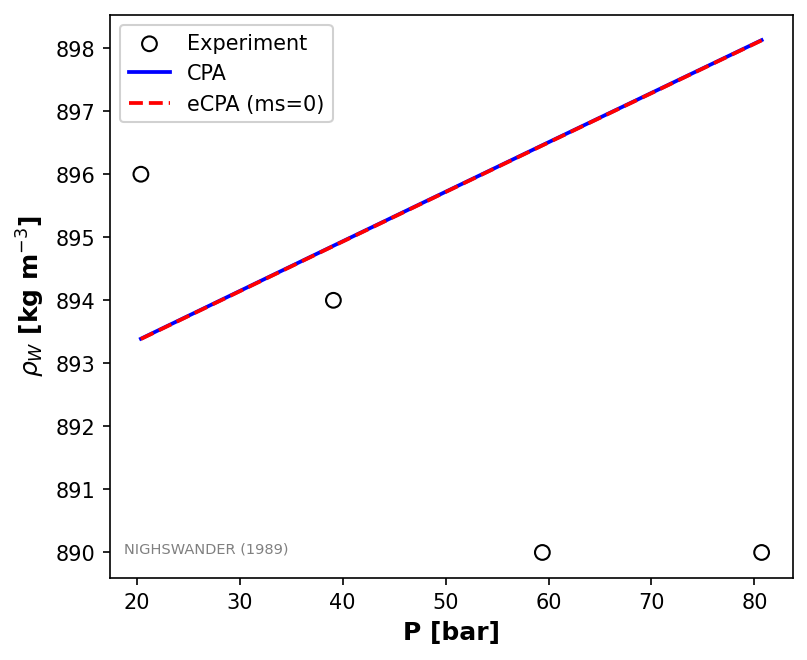
\includegraphics[width=\textwidth]{../figures/density/T433K.png}
    \caption{$T = 433$\,K}
  \end{subfigure}\hfill
  \vspace{4pt}
  \begin{subfigure}[t]{\textwidth}
    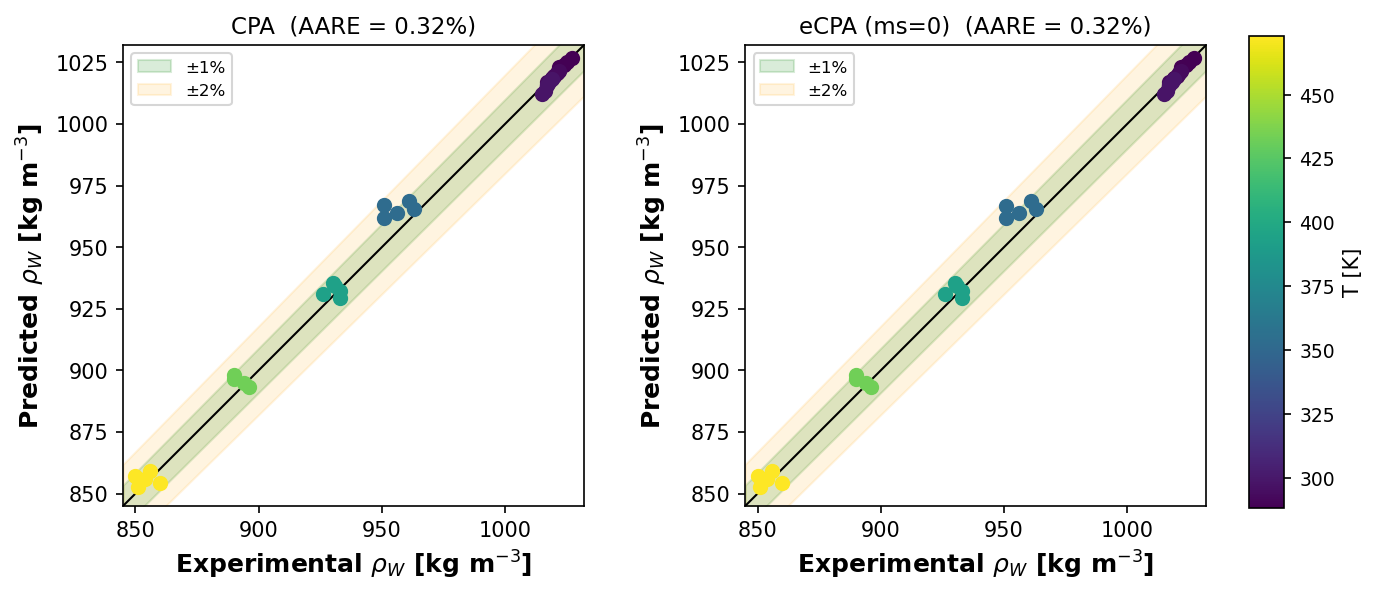
\includegraphics[width=\textwidth]{../figures/density/parity.png}
    \caption{Parity (all $T$)}
  \end{subfigure}
  \caption{Aqueous-phase density of CO$_2$-saturated water (ms~=~0) with optimized
           Péneloux H$_2$O shift ($c_{\text{H}_2\text{O}} = 0.11$\,cm$^3$\,mol$^{-1}$).
           Open circles: experimental data \citep{King1992, Nighswander1989};
           solid line: CPA; dashed line: eCPA.
           The parity plot shows all 37 points colored by temperature.}
  \label{fig:density}
\end{figure}


%% ============================================================
\section{Computational Performance}
\label{sec:performance}

\subsection{Comparison of flash strategies}
\label{sec:benchmark}

Table~\ref{tab:benchmark} compares the wall time and SSI iteration count of four flash
strategies, evaluated at $T = 398$\,K, $z_{\text{CO}_2} = 0.5$, $m_s = 1.0$\,mol\,kg$^{-1}$,
over 30 pressure points spanning 1--1500\,bar.
All times are single-threaded on a modern workstation.

\begin{table}[htb]
  \centering
  \caption{Benchmark of flash strategies at $T = 398$\,K, $z_{\text{CO}_2} = 0.5$,
           $m_s = 1.0$\,mol\,kg$^{-1}$, 30 pressure points.}
  \label{tab:benchmark}
  \begin{tabular}{lrrrr}
    \toprule
    Strategy & Mean iters & Total time & Time/call & Speedup \\
    \midrule
    Cold SSI ($\omega = 0.7$, Wilson init) & 11.7 & 0.30\,s & 10\,ms & 1.0$\times$ (baseline) \\
    Fast: table hint, stability skipped     & 3.3  & 0.09\,s & 3\,ms  & \textbf{3.2}$\times$ \\
    Fast + forced stability check           & 3.3  & 0.54\,s & 18\,ms & 0.6$\times$ \\
    \bottomrule
  \end{tabular}
\end{table}

The fast flash with selective stability checking achieves a 3.2$\times$ speedup over cold-start
SSI.
Forcing the stability test on every call negates this advantage entirely: the Michelsen TPD
evaluation ($\sim$30\,ms per call) costs approximately five times the warm-started flash
($\sim$6\,ms per call).
This motivates the selective strategy: skip the stability test for cells pre-classified as
two-phase by the table, and run it only for cells near the two-phase boundary or on first
call.

\subsection{Flash convergence statistics}
\label{sec:convergence}

Table~\ref{tab:convergence} summarises SSI iteration counts and wall times over the full
validation set, for both the salt-free binary (Rachford--Rice SSI) and the ternary eCPA.

\begin{table}[htb]
  \centering
  \caption{Flash convergence statistics across all validation data.
           Brent $\omega$: damping factor; SSI iterations include both outer (K-value) iterations.}
  \label{tab:convergence}
  \begin{tabular}{llrrrrr}
    \toprule
    System & Method & $N$ calls & Mean iter & Median & Max & Mean time/call \\
    \midrule
    CO$_2$+H$_2$O  & CPA (Rachford--Rice SSI) & 631  & 63.4  & 17  & 1000 & $\sim$100\,ms \\
    CO$_2$+H$_2$O  & eCPA (warm SSI)           & 631  & 2.0   & 2   & 9    & $\sim$25\,ms  \\
    CO$_2$+NaCl    & eCPA (warm SSI)           & 423  & 8.0   & 8   & 14   & $\sim$26\,ms  \\
    \bottomrule
  \end{tabular}
\end{table}

The large mean iteration count for the salt-free CPA binary (63.4 vs.\ median 17) reflects
a few slow-converging points near the CO$_2$ critical pressure ($P \approx 74$\,bar at
$T = 304$\,K), where the K-values exhibit large gradients and simple SSI with damping
requires many iterations.
The eCPA warm-started SSI is dramatically more efficient (mean 2.0 iterations) because the
table guess is already close to the solution.
The ternary system requires more iterations on average (8 vs.\ 2) because the molality
dimension adds a degree of freedom not directly table-interpolated, but convergence remains
robust and fast.


%% ============================================================
\section{Reservoir Simulation Demonstration}
\label{sec:simulator}

To illustrate the practical applicability of the fast eCPA flash routine in a reservoir
simulation context, we implemented a minimal but complete isothermal compositional
simulator for CO$_2$ injection into a 2D saline aquifer.

\subsection{Numerical scheme}
\label{sec:sim_scheme}

The simulator uses a standard IMPEC (implicit-pressure, explicit-composition) scheme
\citep{Lie2019} on a uniform Cartesian grid.
Pressure is solved implicitly at each time step via a two-point flux approximation (TPFA)
\citep{Aavatsmark2003}, yielding Darcy velocities that drive the explicit advection of the
overall CO$_2$ mole fraction $z$.
The transport sub-step size is constrained by a CFL condition based on the maximum
derivative of the molar fractional flow $\partial F_z / \partial z$, estimated by a
one-dimensional scan at startup.

The physical model includes two mobile phases (aqueous and CO$_2$-rich) with Corey
relative permeabilities, and interphase CO$_2$/H$_2$O transfer computed by calling
\texttt{flash\_co2\_h2o\_salt\_fast} at every grid cell every time step.
NaCl is treated as non-volatile; its equilibrium aqueous molality $m_s^\mathrm{aq}$,
which exceeds the nominal feed molality in two-phase cells (salting-out effect), is
returned by the flash and carried forward to the saturation calculation.

We deliberately neglect the density dependence of the pressure equation, replacing the
true compressible flux divergence by the volume-rate constraint $\nabla\cdot\mathbf{u} = q$.
This is non-physical---real CO$_2$--brine systems are weakly compressible and the
density contrast between phases drives buoyancy---but it is sufficient for our purpose,
which is to demonstrate the robustness and efficiency of the flash routine in a
time-stepping loop, not to produce quantitatively predictive reservoir simulations.
Readers wishing to deploy the flash in production-grade simulators can integrate it
directly into open-source codes such as the MATLAB Reservoir Simulation Toolbox
(MRST, \citealt{Lie2019}), OPM Flow \citep{Rasmussen2021}, or DuMu$^x$ \citep{Koch2021},
all of which expose user-supplied flash callbacks or component-level EoS interfaces.

\subsection{Simulation setup}
\label{sec:sim_setup}

The domain is a $100\times100$\,m$^2$ square with a 10\,m thickness, discretized onto a
$50\times50$ Cartesian grid ($N = 2500$ cells).
Permeability is uniform at 100\,mD and porosity is 0.20.
A five-spot well pattern is used: one injector at the domain center and four producers
at the corners, with CO$_2$ injected at 10\% of total pore volume per year.
The simulation runs for 3 years at $T = 350$\,K, $P = 200$\,bar, and an initial NaCl
molality of $m_s = 1.0$\,mol\,kg$^{-1}$.

\subsection{Results}
\label{sec:sim_results}

Figure~\ref{fig:simulator} shows the CO$_2$-rich phase saturation $S_g$ at three
representative times.
The plume grows radially from the injector, progressively sweeping toward the corner
producers.
At early time (panel a, $t = 0.36$\,yr) significant grid-orientation effects, inherent to
TPFA on Cartesian grids and well documented in the literature \citep{Aavatsmark2003},
are visible in the diamond-shaped front.
This is a known limitation of TPFA and can be reduced by using multi-point flux
approximation (MPFA) schemes \citep{Aavatsmark2003} or unstructured grids; we note it
here only to be transparent about the numerics, since our goal is to demonstrate the
flash rather than the flow solver.
At later times the front smooths out as the plume grows beyond a few grid spacings.

\begin{figure}[htb]
  \centering
  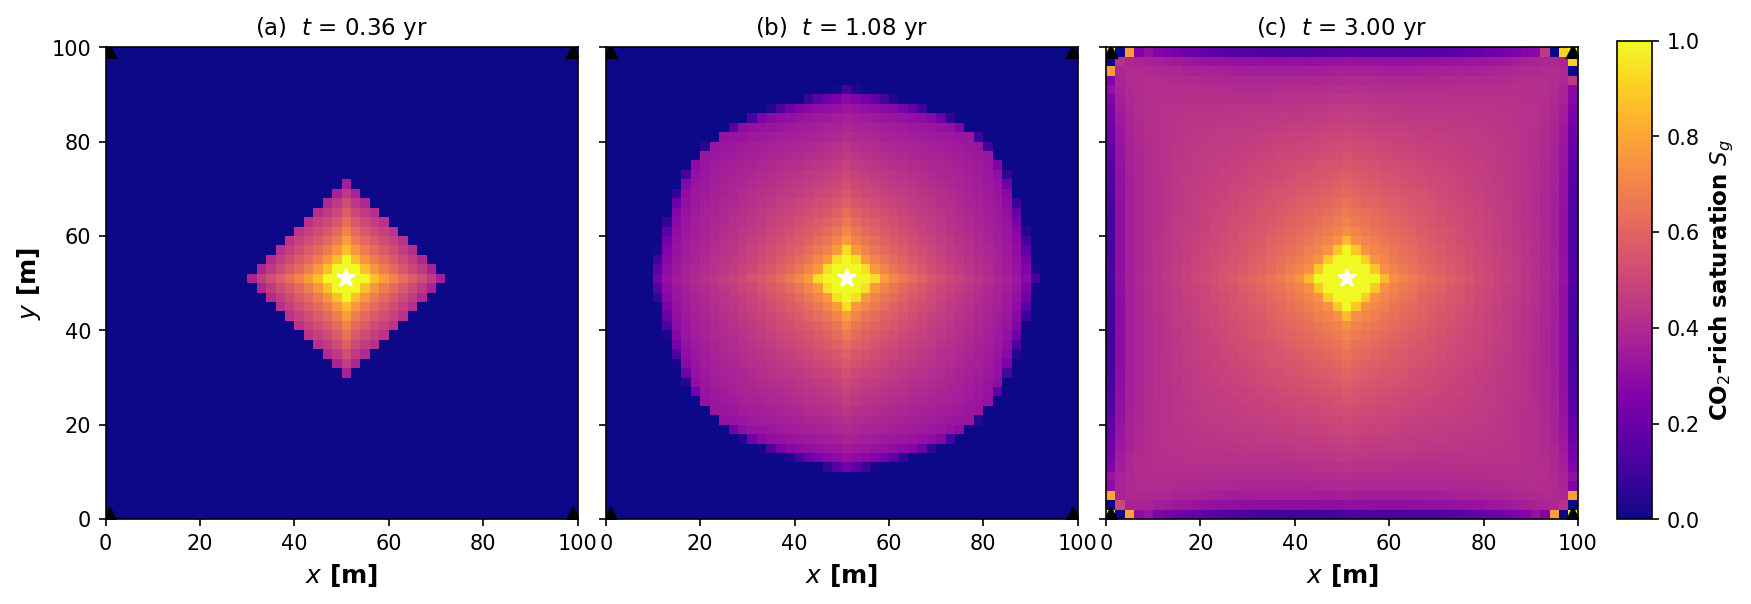
\includegraphics[width=\textwidth]{../figures/simulator/fig_simulator.png}
  \caption{CO$_2$-rich saturation $S_g$ at three simulation times for a $50\times50$
           Cartesian grid ($T = 350$\,K, $P = 200$\,bar, $m_s = 1.0$\,mol\,kg$^{-1}$).
           White star: CO$_2$ injector; black triangles: producers.
           The diamond shape at early time (panel a) reflects the well-known
           grid-orientation sensitivity of TPFA.}
  \label{fig:simulator}
\end{figure}

Figure~\ref{fig:compositions} shows the three compositional quantities returned by the
eCPA flash at each time step: the equilibrium brine salinity $m_s^\mathrm{aq}$, the
CO$_2$ mole fraction in the aqueous phase $x_{\text{CO}_2}$, and the H$_2$O mole
fraction in the CO$_2$-rich phase $y_{\text{H}_2\text{O}}$.
These fields have no counterpart in a conventional black-oil simulator and are the
direct output of the compositional eCPA flash at each grid cell.

The brine salinity map (panels a, d) reveals the \emph{salting-out} effect: as CO$_2$
displaces water from pore space, the remaining brine becomes more concentrated in NaCl.
The salting-out is strongest where $S_g$ is largest (near the injector), producing the
vivid radial gradient from 1.0\,mol\,kg$^{-1}$ (background) toward the
colour-saturated maximum (cells adjacent to the pure-CO$_2$ injector zone, which
appears pale because the brine has been fully expelled).
The gradient broadens from $t = 1.08$\,yr (panel a) to $t = 3.00$\,yr (panel d) as the
high-saturation zone expands.

The CO$_2$ dissolution map (panels b, e) shows the two-phase zone extent: inside the
plume the aqueous phase is CO$_2$-saturated at the eCPA equilibrium value
($x_{\text{CO}_2} \approx 0.016$ at $T = 350$\,K, $P = 200$\,bar, $m_s \approx 1$\,mol\,kg$^{-1}$),
while outside the plume the brine remains essentially CO$_2$-free.
Similarly, panels (c, f) show that the CO$_2$-rich phase everywhere in the plume
contains the eCPA-predicted equilibrium water content
($y_{\text{H}_2\text{O}} \approx 0.010$).
The spatial uniformity of $x_{\text{CO}_2}$ and $y_{\text{H}_2\text{O}}$ within the
plume is physically correct for this isothermal, isobaric model: thermodynamic
equilibrium dictates that the phase compositions depend only on $(T, P, m_s)$, which
are nearly uniform away from the salting-out gradient.
In a real simulation with temperature and pressure gradients, these fields would exhibit
richer spatial structure.

\begin{figure}[htb]
  \centering
  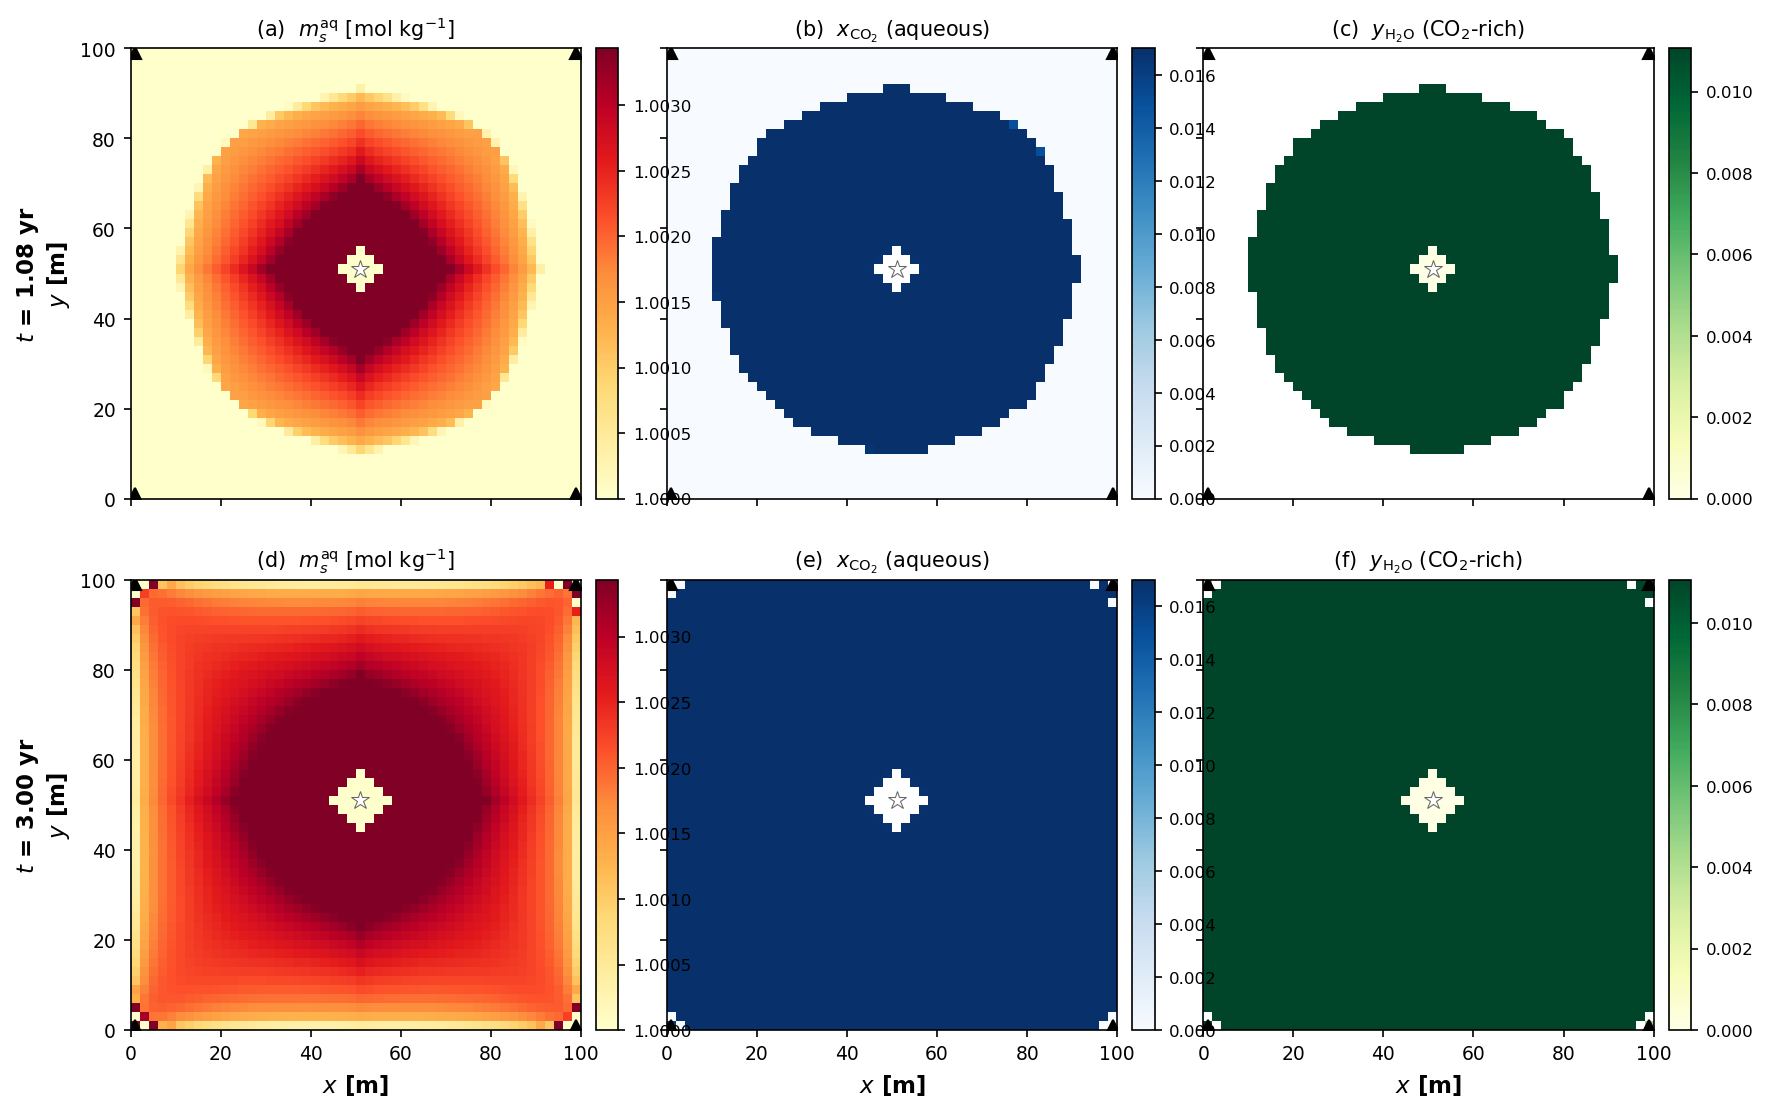
\includegraphics[width=\textwidth]{../figures/simulator/fig_compositions.png}
  \caption{Compositional flash outputs at $t = 1.08$\,yr (top row) and $t = 3.00$\,yr
           (bottom row).
           \textbf{(a, d)} Equilibrium brine salinity $m_s^\mathrm{aq}$: the smooth
           radial gradient reflects salting-out proportional to CO$_2$ saturation;
           the pale region near the injector is the pure-CO$_2$ cell cluster where
           brine is absent.
           Colorbar is clipped at the 80th-percentile value to make the gradient
           visible across the domain; cells near the injector exceed the colorbar
           maximum.
           \textbf{(b, e)} CO$_2$ mole fraction in the aqueous phase $x_{\text{CO}_2}$:
           the plume interior (dark) is CO$_2$-saturated at the eCPA equilibrium value
           (${\approx}0.016$); the exterior (pale) is essentially CO$_2$-free.
           \textbf{(c, f)} H$_2$O mole fraction in the CO$_2$-rich phase
           $y_{\text{H}_2\text{O}}$: the plume carries ${\approx}1$\% water throughout,
           consistent with the eCPA prediction at these conditions.
           White star: injector; black triangles: producers.}
  \label{fig:compositions}
\end{figure}

\subsection{Flash performance in the simulator}
\label{sec:sim_perf}

Figure~\ref{fig:sim_perf} shows the wall time per time step and the number of flash calls
as a function of simulation time.
Flash dominates the total step cost throughout the run: the blue and dashed curves
(flash time and total step time) are nearly coincident.
The number of two-phase cells grows steadily as CO$_2$ spreads, peaking near 2500 (all
cells) around $t \approx 2.5$\,yr before falling slightly as producers sweep the domain.

\begin{figure}[htb]
  \centering
  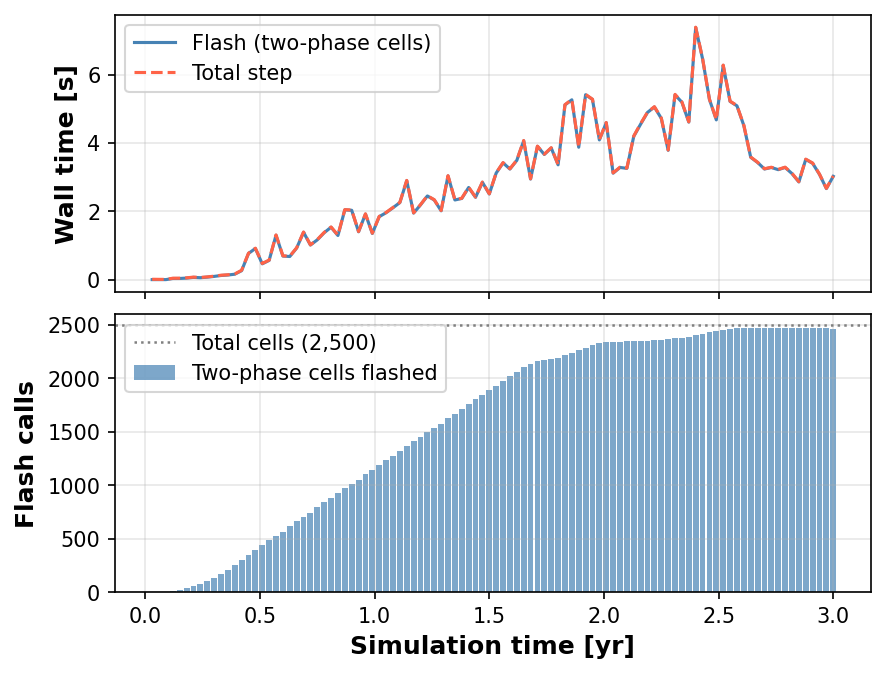
\includegraphics[width=0.72\textwidth]{../figures/simulator/fig_perf.png}
  \caption{Simulator performance over 100 time steps (3 yr).
           \emph{Top}: wall time for the flash (two-phase cells only) and the complete
           time step.
           \emph{Bottom}: number of cells dispatched to the eCPA flash per step, with
           the total cell count (2500) shown as a dotted reference.
           Flash accounts for $\gtrsim 90$\% of total step cost at all times.}
  \label{fig:sim_perf}
\end{figure}

Table~\ref{tab:sim_perf} summarizes the aggregate flash performance.
The measured throughput of 713 flash calls per second (multi-core, Python
\texttt{multiprocessing}) demonstrates that the warm-started eCPA flash is
fast enough to sustain a 2500-cell compositional simulation at 2.45\,s per step,
with flash accounting for essentially all of that cost.
Scaling to larger grids ($10^5$--$10^6$ cells) would benefit from compiled
implementations or GPU acceleration of the innermost EoS evaluations, but the
algorithmic speedup demonstrated here---$3.2\times$ over cold-start SSI---applies
equally at any scale.

\begin{table}[htb]
  \centering
  \caption{Aggregate flash performance across the 3-year simulation
           ($50\times50$ grid, $T = 350$\,K, $P = 200$\,bar, $m_s = 1.0$\,mol\,kg$^{-1}$,
           multi-core Python).}
  \label{tab:sim_perf}
  \begin{tabular}{lr}
    \toprule
    Metric & Value \\
    \midrule
    Grid cells & 2500 \\
    Time steps & 100 \\
    Mean two-phase cells / step & 1585 (max 2472) \\
    Mean flash wall time / step & 2.45\,s \\
    Flash fraction of step cost & $\approx 100$\% \\
    Flash throughput (multi-core) & 713 calls\,s$^{-1}$ \\
    \bottomrule
  \end{tabular}
\end{table}


%% ============================================================
\section{Conclusions}
\label{sec:conclusions}

We have developed and validated an open-source Python implementation of phase stability and
flash calculations for CO$_2$ + H$_2$O + NaCl mixures using the eCPA equation of state of
\citet{Coelho2025}.
Key conclusions are:

\begin{enumerate}
  \item The eCPA EoS implemented in this work accurately reproduces
        experimental CO$_2$ solubility data in pure water (AARE 8.2\%) and NaCl brine
        (AARE 6.9\% overall, rising to $\sim$14\% at hydrothermal conditions $T > 550$\,K).

  \item A generalized salt-free CPA flash routine with full Michelsen
        stability + SSI was developed independently and validated against the same binary
        dataset.
        Both models agree within their respective parameterization accuracy.

  \item A precomputed four-dimensional solution table (31T $\times$ 30P $\times$ 18$z$ $\times$
        14$m_s$ = 234{,}360 cells, all filled, $T = 283$--$728$\,K, $P = 1$--$1500$\,bar,
        $m_s = 0$--$6$\,mol\,kg$^{-1}$)
        enables warm-started flash that converges in 3--4 iterations compared to 12 for cold-start
        SSI, achieving a 3.2$\times$ speedup without loss of accuracy.

  \item An optimized Péneloux volume shift for water ($c_{\text{H}_2\text{O}} = 0.11$\,cm$^3$\,mol$^{-1}$)
        reduces aqueous-phase density AARE from 0.76\% to 0.33\% (37 data points, $T = 288$--$473$\,K),
        an original improvement beyond the published eCPA model.

  \item A minimal IMPEC compositional reservoir simulator demonstrates that the warm-started
        eCPA flash sustains a $50\times50$-cell CO$_2$ injection simulation at
        $\sim$600 flash calls\,s$^{-1}$ (multi-core Python), with flash accounting
        for $\gtrsim 90$\% of total step cost.
        The flash routine can be integrated into production-grade open-source simulators
        such as MRST \citep{Lie2019}, OPM Flow \citep{Rasmussen2021}, or
        DuMu$^\mathrm{x}$ \citep{Koch2021}.

  \item All code is released open-source and described in the Supplemental Information.
        The implementation is designed for direct use in reservoir simulation pipelines via
        the fast flash routine described in Section~\ref{sec:fast_flash}.
\end{enumerate}


%% ============================================================
\section*{Acknowledgements}

%% TODO: fill in funding sources, data sources, HPC access, etc.
The authors thank \ldots


%% ============================================================
\appendix
\section{Appendix: EoS Parameters}
\label{sec:params}

For completeness, Tables~\ref{tab:pure_params} and \ref{tab:binary_params} reproduce the
key EoS parameters used in this work, all from \citet{Coelho2025}.

\begin{table}[htb]
  \centering
  \caption{Pure-component CPA/eCPA parameters \citep{Coelho2025}.
           For ions, $a_0 = 0$. H$_2$O uses the 4C association scheme.}
  \label{tab:pure_params}
  \begin{tabular}{lccccccc}
    \toprule
    Species & $a_0$ (J\,m$^3$\,mol$^{-2}$) & $c_1$ & $b$ (cm$^3$\,mol$^{-1}$) &
              $\varepsilon/k_B$ (K) & $\kappa$ & $\sigma$ (\AA) & $R_B$ (\AA) \\
    \midrule
    H$_2$O & 0.1228 & 0.6736 & 14.52 & 2003 & $\kappa^*$ & ---   & ---   \\
    CO$_2$  & 0.3508 & 0.7602 & 27.20 & ---  & ---        & ---   & ---   \\
    Na$^+$  & 0      & ---    & 16.49 & ---  & ---        & 2.356 & 1.665 \\
    Cl$^-$  & 0      & ---    & 40.83 & ---  & ---        & 3.187 & 1.828 \\
    \bottomrule
  \end{tabular}
  \begin{flushleft}
    \footnotesize $^*\kappa = \kappa_{\text{assoc}} \cdot b_{\text{H}_2\text{O}}$,
    $\kappa_{\text{assoc}} = 69.2 \times 10^{-3}$.
  \end{flushleft}
\end{table}

\begin{table}[htb]
  \centering
  \caption{Temperature-dependent binary interaction parameters \citep{Coelho2025}.
           $X = A_X(T/T_{c,c})^2 + B_X(T/T_{c,c}) + C_X$, $T_{c,c} = 304.4$\,K.}
  \label{tab:binary_params}
  \begin{tabular}{lrrr}
    \toprule
    Parameter & $A$ & $B$ & $C$ \\
    \midrule
    $k_{cw}$ (CO$_2$--H$_2$O binary interaction parameter) & $-0.492$ & $2.101$ & $-1.571$ \\
    $S_{cw}$ (cross-assoc.\ strength) & $+0.192$ & $-0.173$ & $-0.009$ \\
    \bottomrule
  \end{tabular}

  \vspace{6pt}
  \begin{tabular}{lrrrr}
    \toprule
    Ion--neutral pair & $\Delta U^{\text{ref}}$ (J\,mol$^{-1}$) & $\alpha$ (K) & $T^\alpha$ (K) & Source \\
    \midrule
    H$_2$O--NaCl ($\Delta U_{ws}$) & $-1858$ & 1573 & 340 & Maribo-Mogensen et al.\ (2015) \\
    CO$_2$--NaCl ($\Delta U_{cs}$) & $+6056$ & 692  & 244 & \citet{Coelho2025} \\
    \bottomrule
  \end{tabular}
\end{table}


%% ============================================================
\bibliographystyle{elsarticle-harv}
\bibliography{refs}


%% ============================================================
%% SUPPLEMENTAL INFORMATION
%% ============================================================
\appendix

\section*{Supplemental Information}
\label{sec:si}

\setcounter{section}{0}
\setcounter{figure}{0}
\renewcommand{\thesection}{S\arabic{section}}
\renewcommand{\thefigure}{S\arabic{figure}}

%% --- SI Figure S1: all CO2+H2O panels ---
\begin{figure}[p]
  \centering
  \newcommand{\swsi}{0.235\textwidth}%
  \begin{subfigure}[t]{\swsi}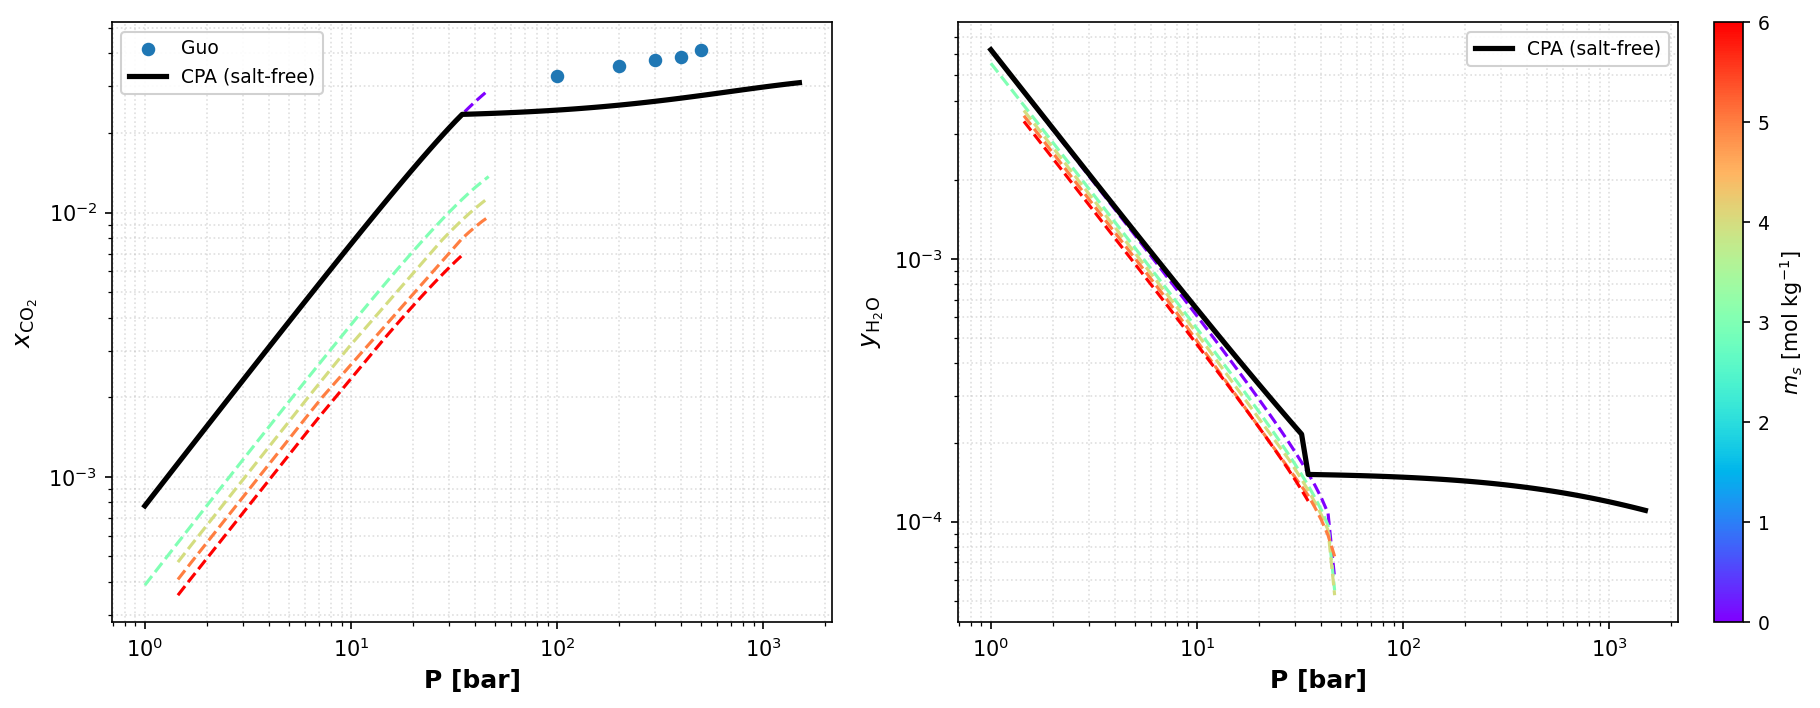
\includegraphics[width=\textwidth]{../figures/co2h2o/T273K.png}\caption{273\,K}\end{subfigure}\hfill
  \begin{subfigure}[t]{\swsi}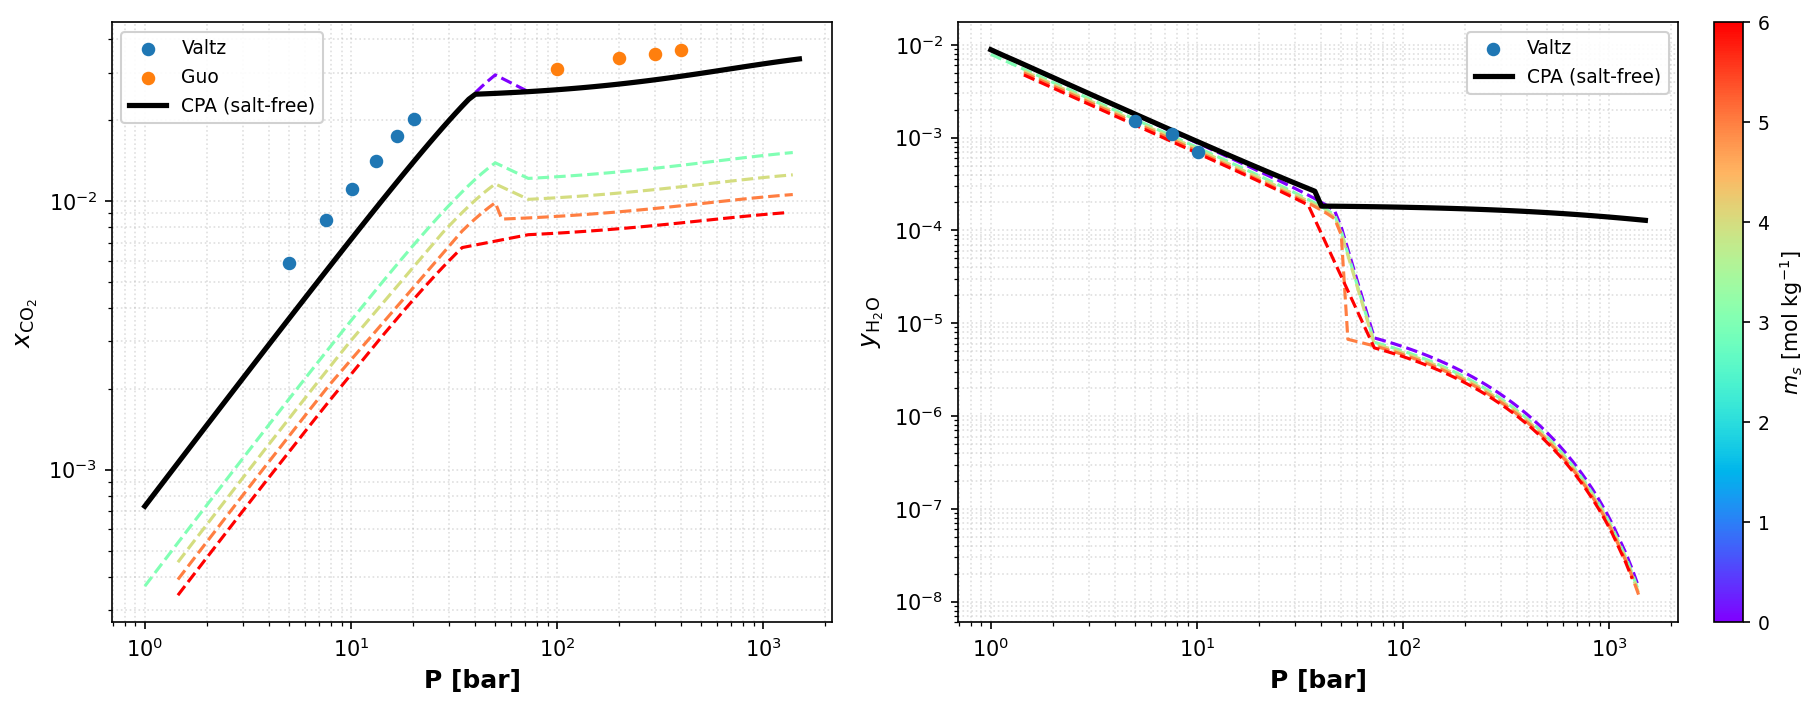
\includegraphics[width=\textwidth]{../figures/co2h2o/T278K.png}\caption{278\,K}\end{subfigure}\hfill
  \begin{subfigure}[t]{\swsi}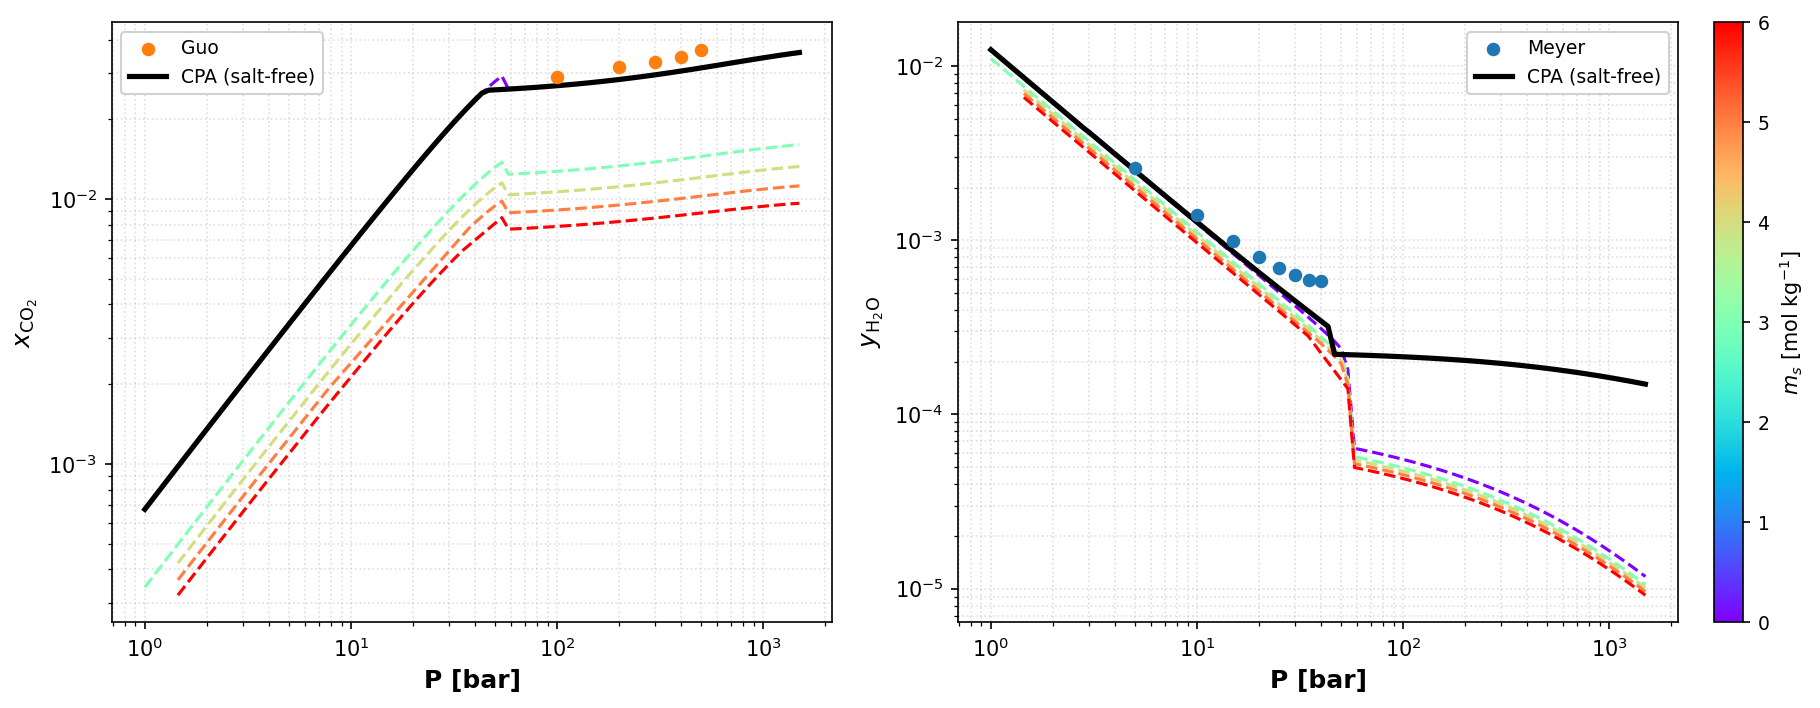
\includegraphics[width=\textwidth]{../figures/co2h2o/T283K.png}\caption{283\,K}\end{subfigure}\hfill
  \begin{subfigure}[t]{\swsi}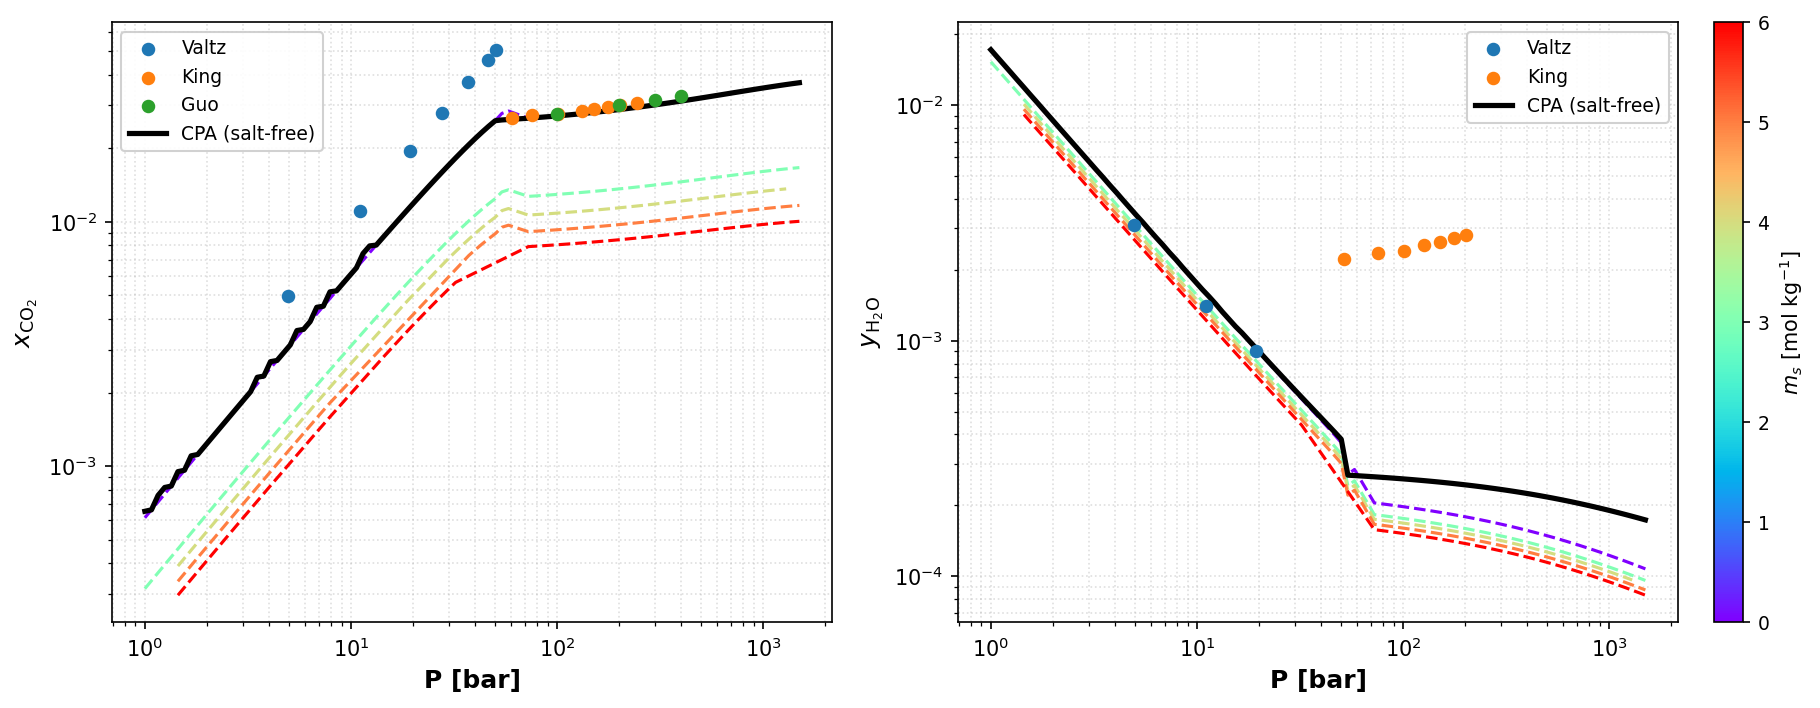
\includegraphics[width=\textwidth]{../figures/co2h2o/T288K.png}\caption{288\,K}\end{subfigure}\\[4pt]
  \begin{subfigure}[t]{\swsi}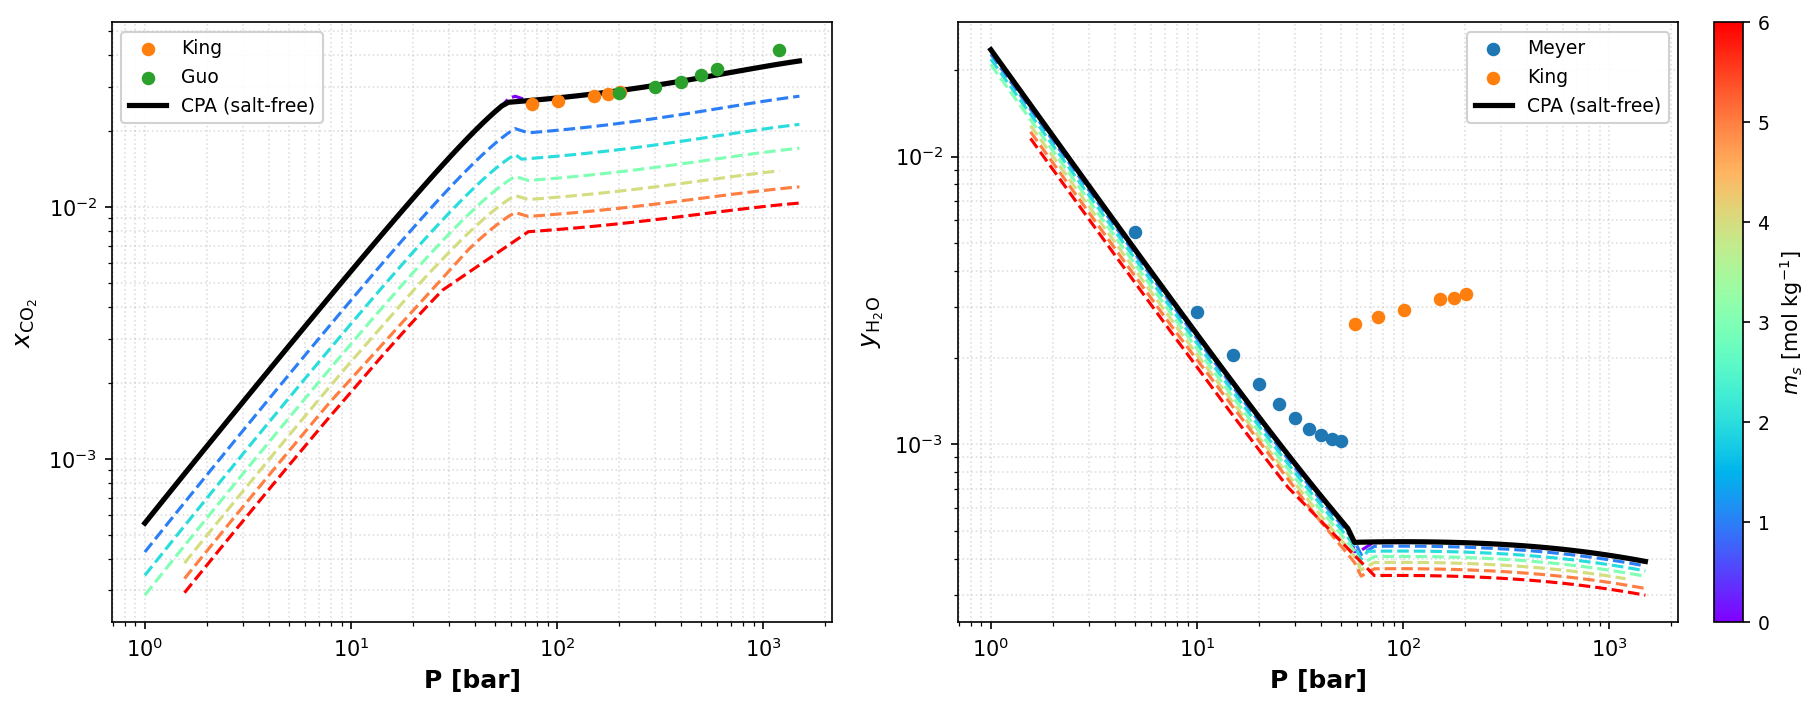
\includegraphics[width=\textwidth]{../figures/co2h2o/T293K.png}\caption{293\,K}\end{subfigure}\hfill
  \begin{subfigure}[t]{\swsi}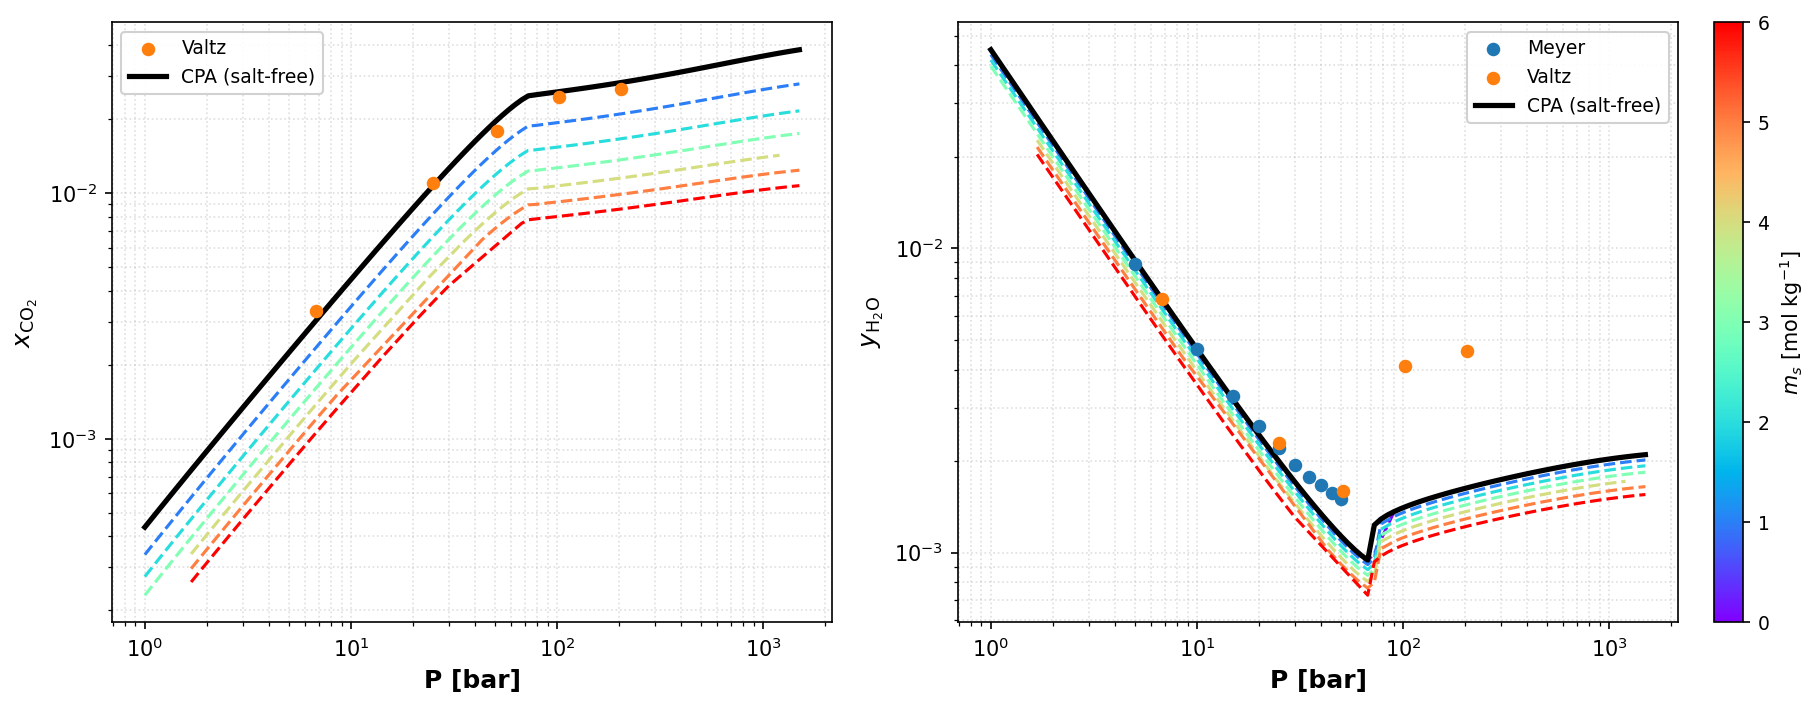
\includegraphics[width=\textwidth]{../figures/co2h2o/T304K.png}\caption{304\,K}\end{subfigure}\hfill
  \begin{subfigure}[t]{\swsi}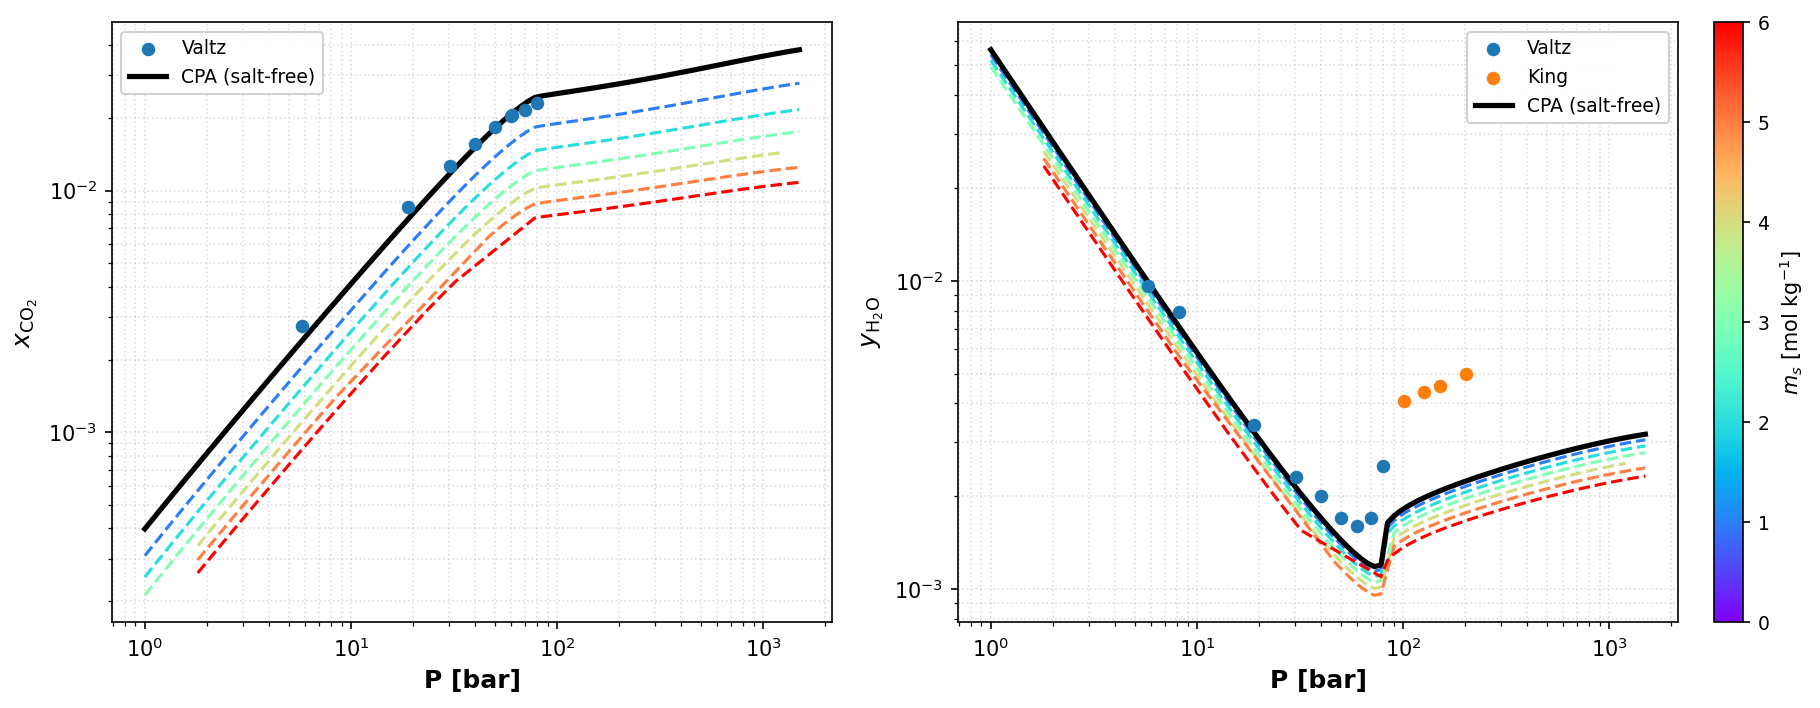
\includegraphics[width=\textwidth]{../figures/co2h2o/T308K.png}\caption{308\,K}\end{subfigure}\hfill
  \begin{subfigure}[t]{\swsi}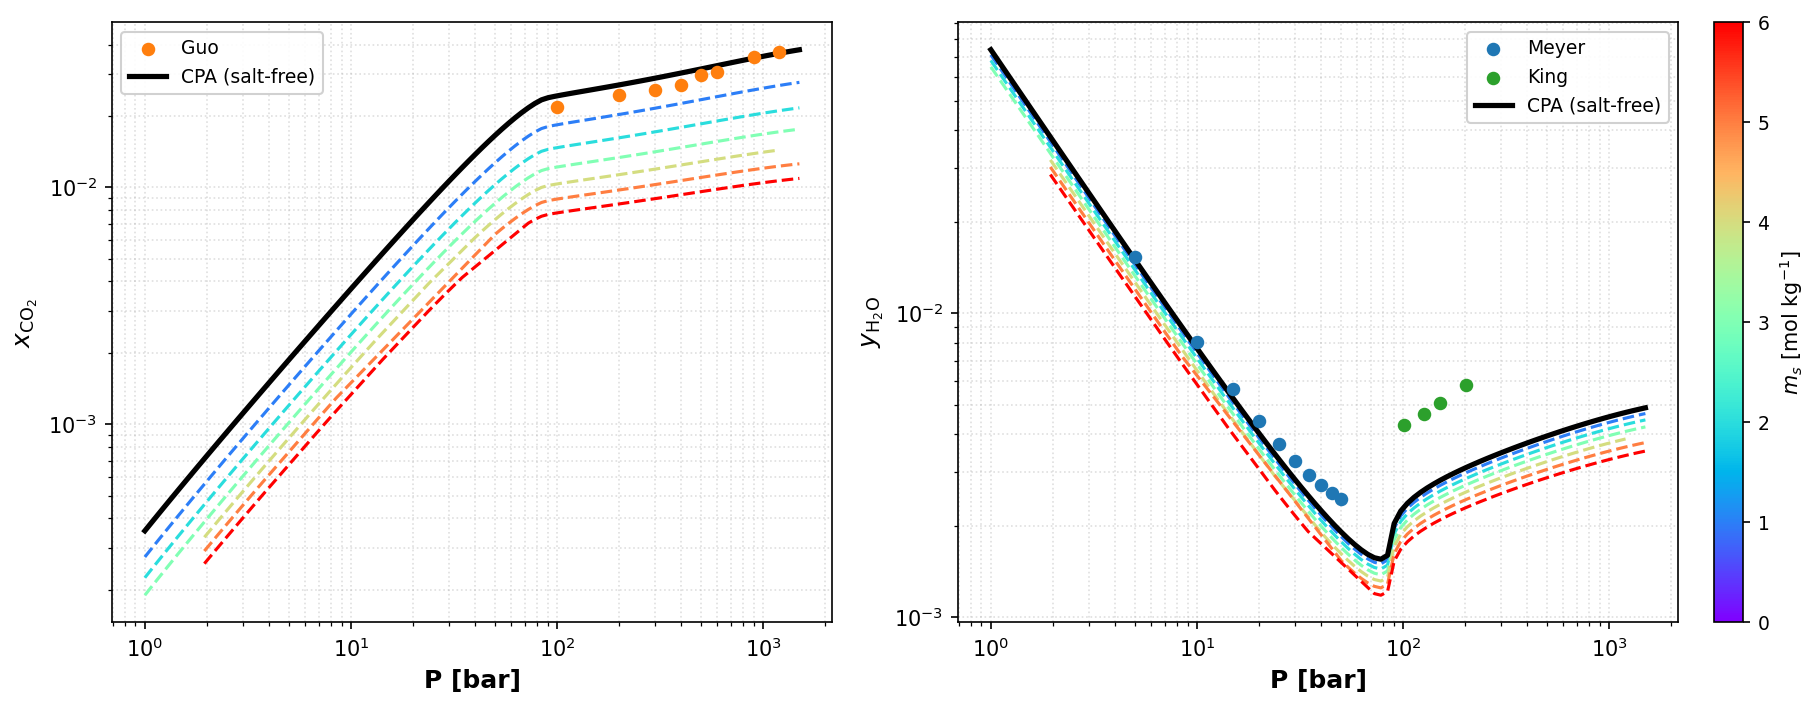
\includegraphics[width=\textwidth]{../figures/co2h2o/T313K.png}\caption{313\,K}\end{subfigure}\\[4pt]
  \begin{subfigure}[t]{\swsi}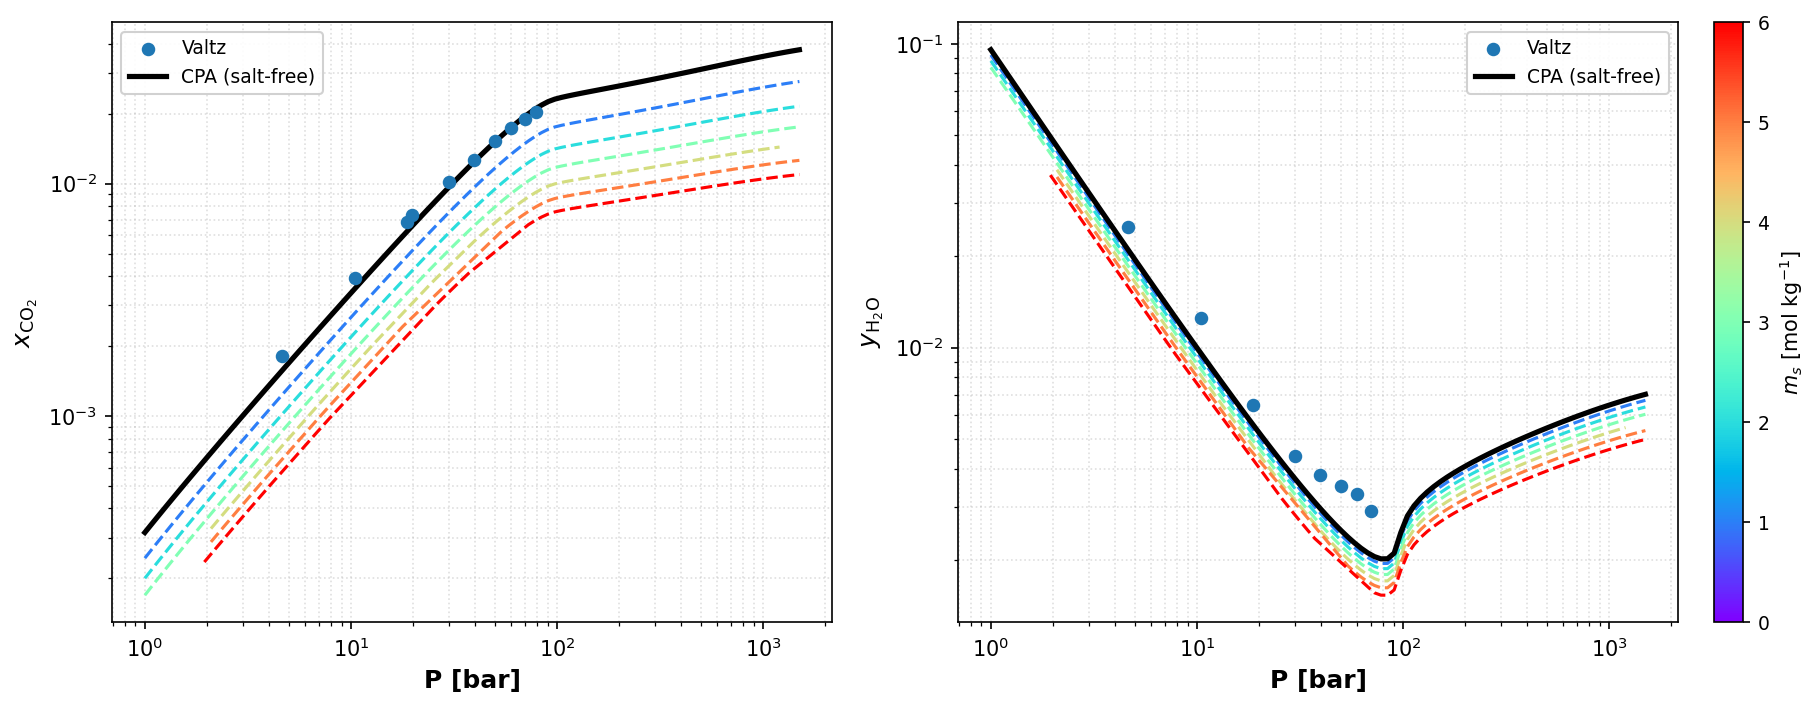
\includegraphics[width=\textwidth]{../figures/co2h2o/T318K.png}\caption{318\,K}\end{subfigure}\hfill
  \begin{subfigure}[t]{\swsi}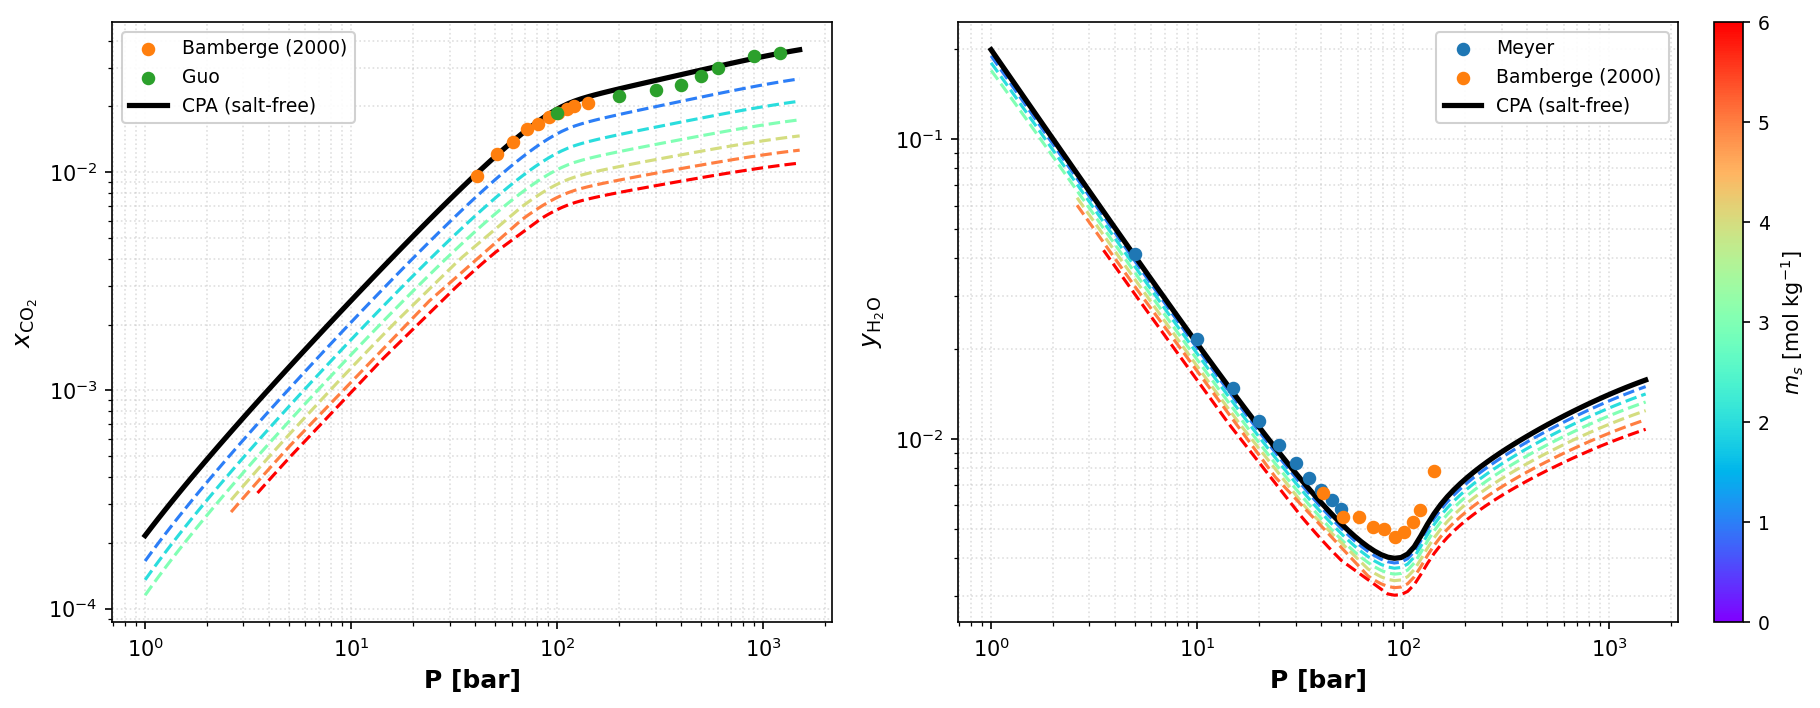
\includegraphics[width=\textwidth]{../figures/co2h2o/T333K.png}\caption{333\,K}\end{subfigure}\hfill
  \begin{subfigure}[t]{\swsi}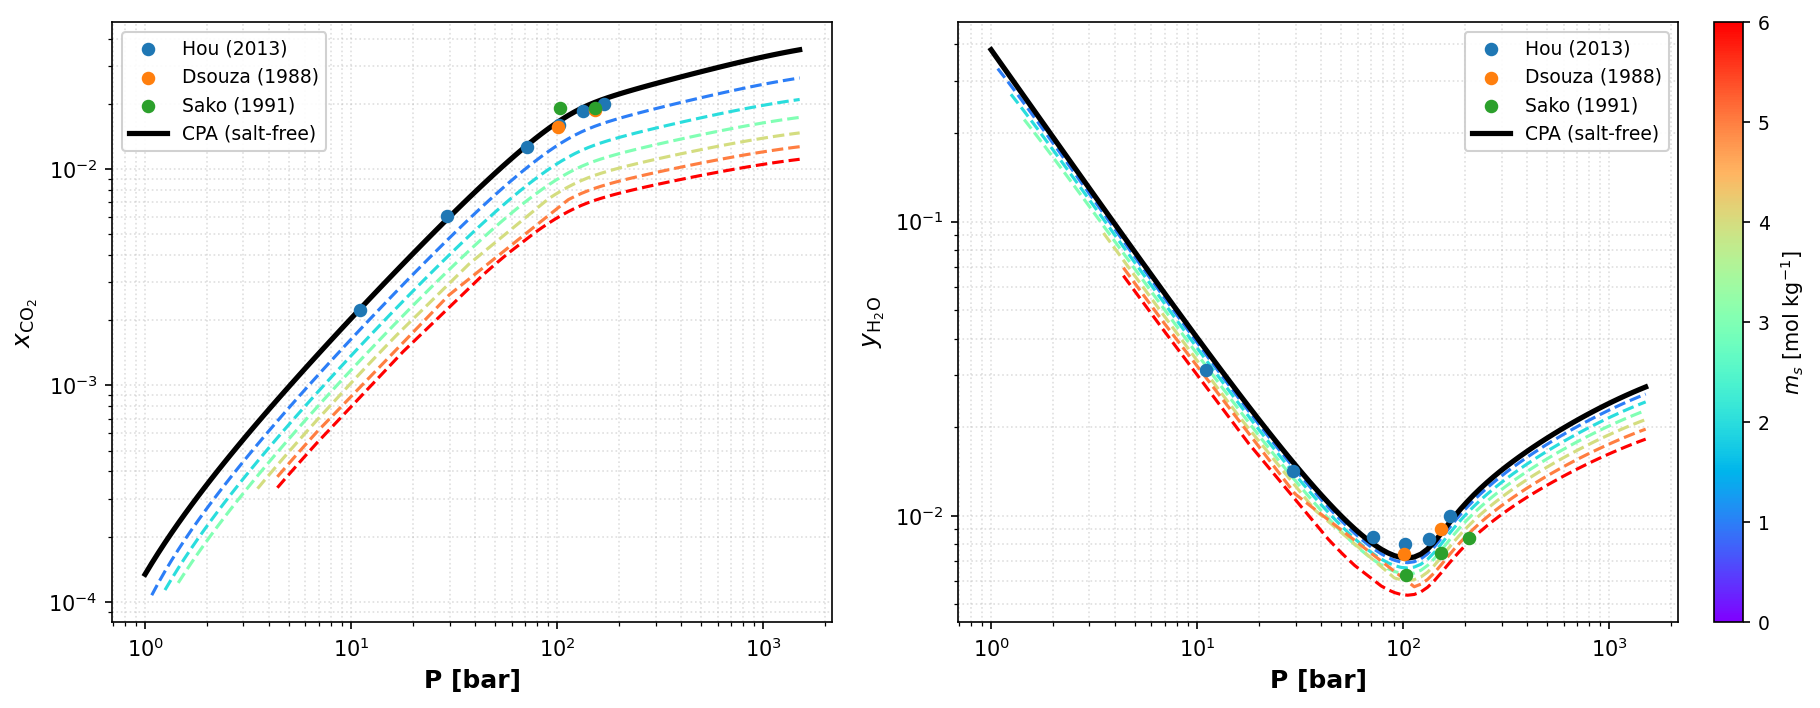
\includegraphics[width=\textwidth]{../figures/co2h2o/T348K.png}\caption{348\,K}\end{subfigure}\hfill
  \begin{subfigure}[t]{\swsi}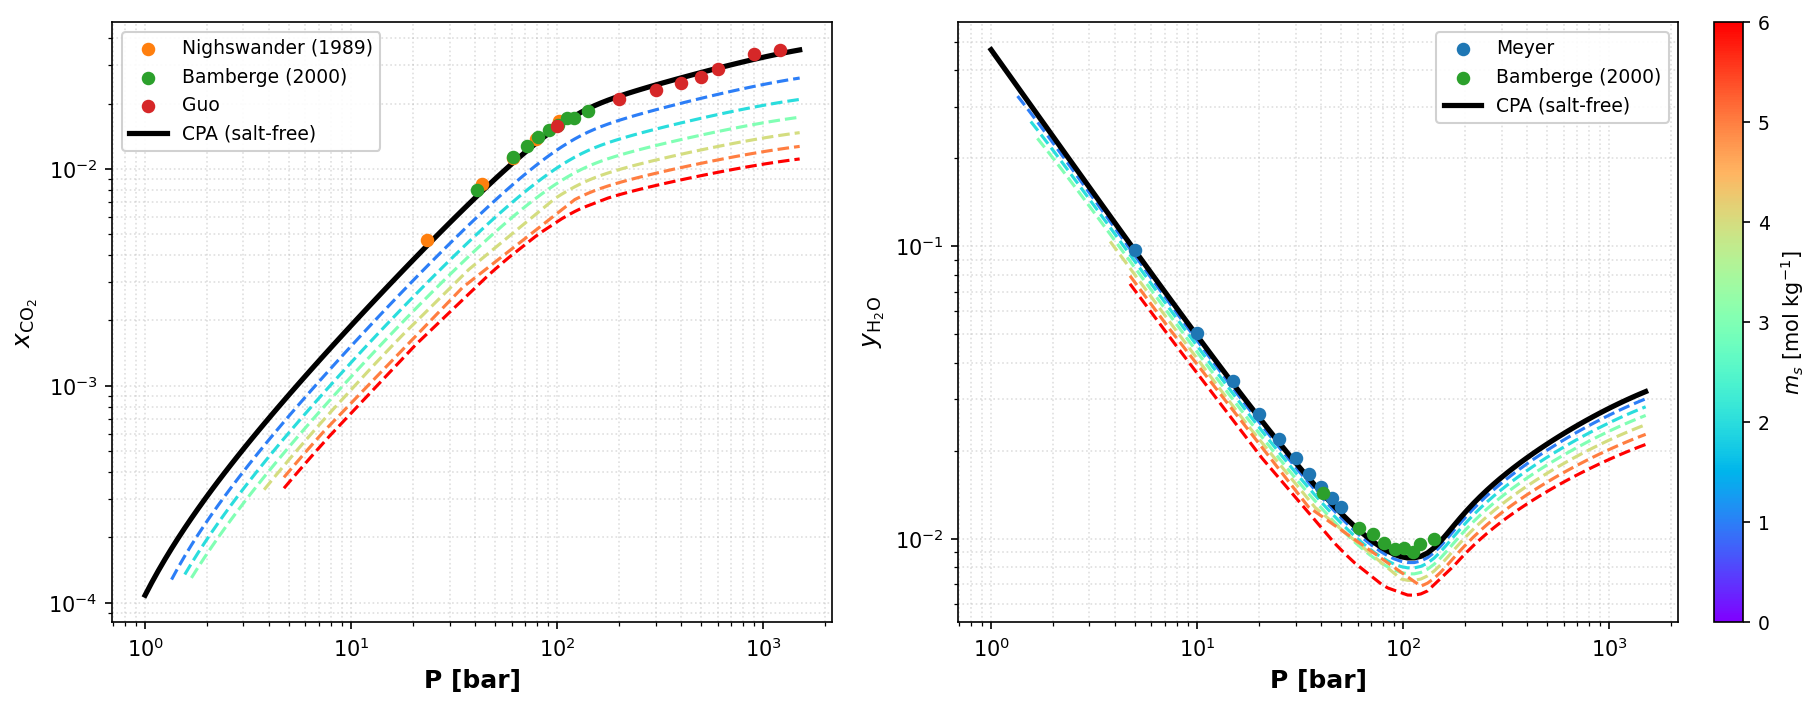
\includegraphics[width=\textwidth]{../figures/co2h2o/T353K.png}\caption{353\,K}\end{subfigure}\\[4pt]
  \begin{subfigure}[t]{\swsi}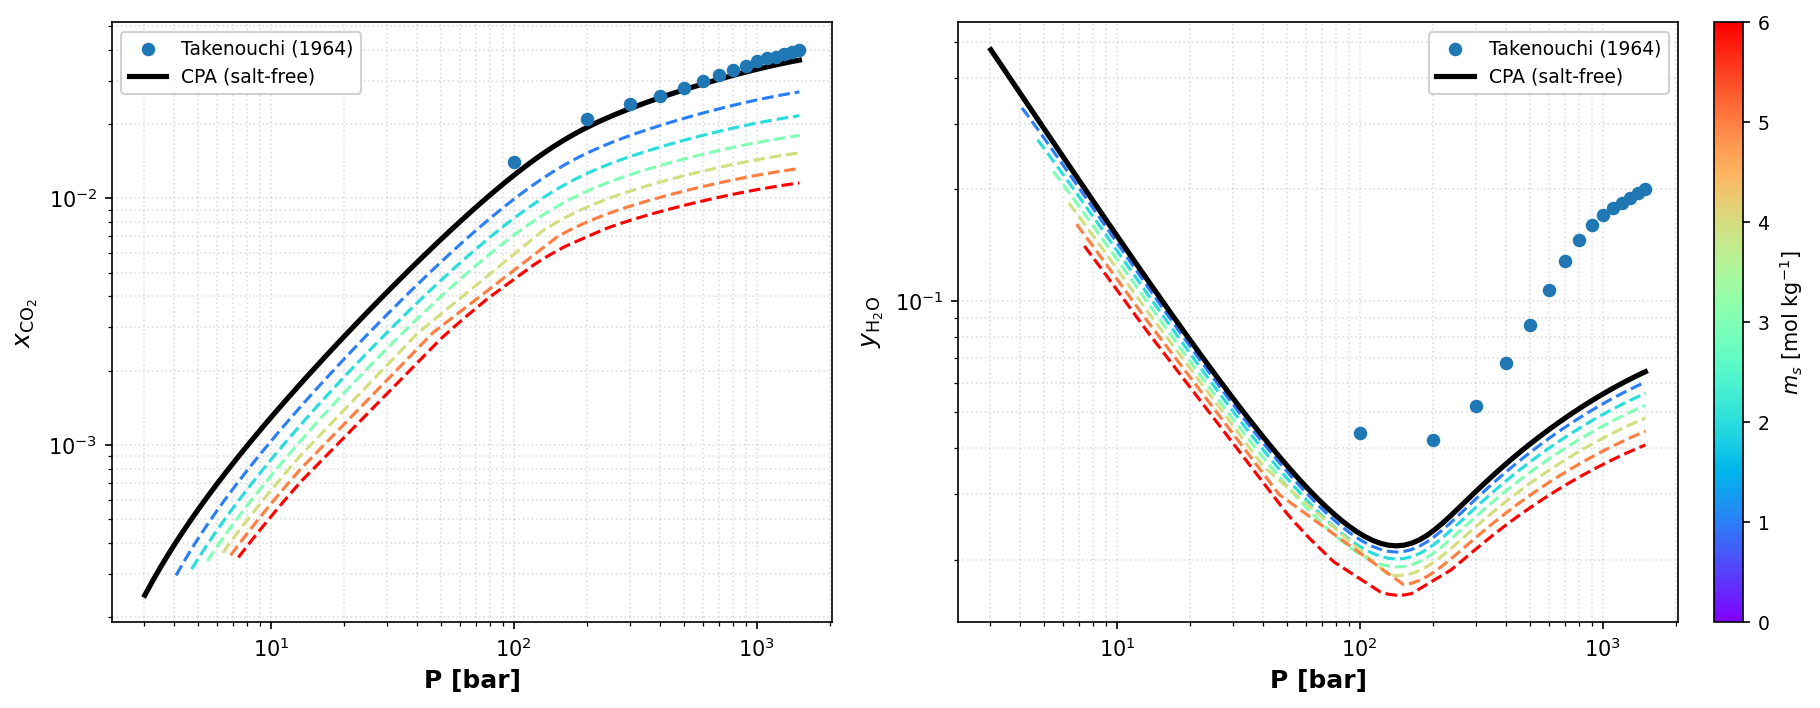
\includegraphics[width=\textwidth]{../figures/co2h2o/T383K.png}\caption{383\,K}\end{subfigure}\hfill
  \begin{subfigure}[t]{\swsi}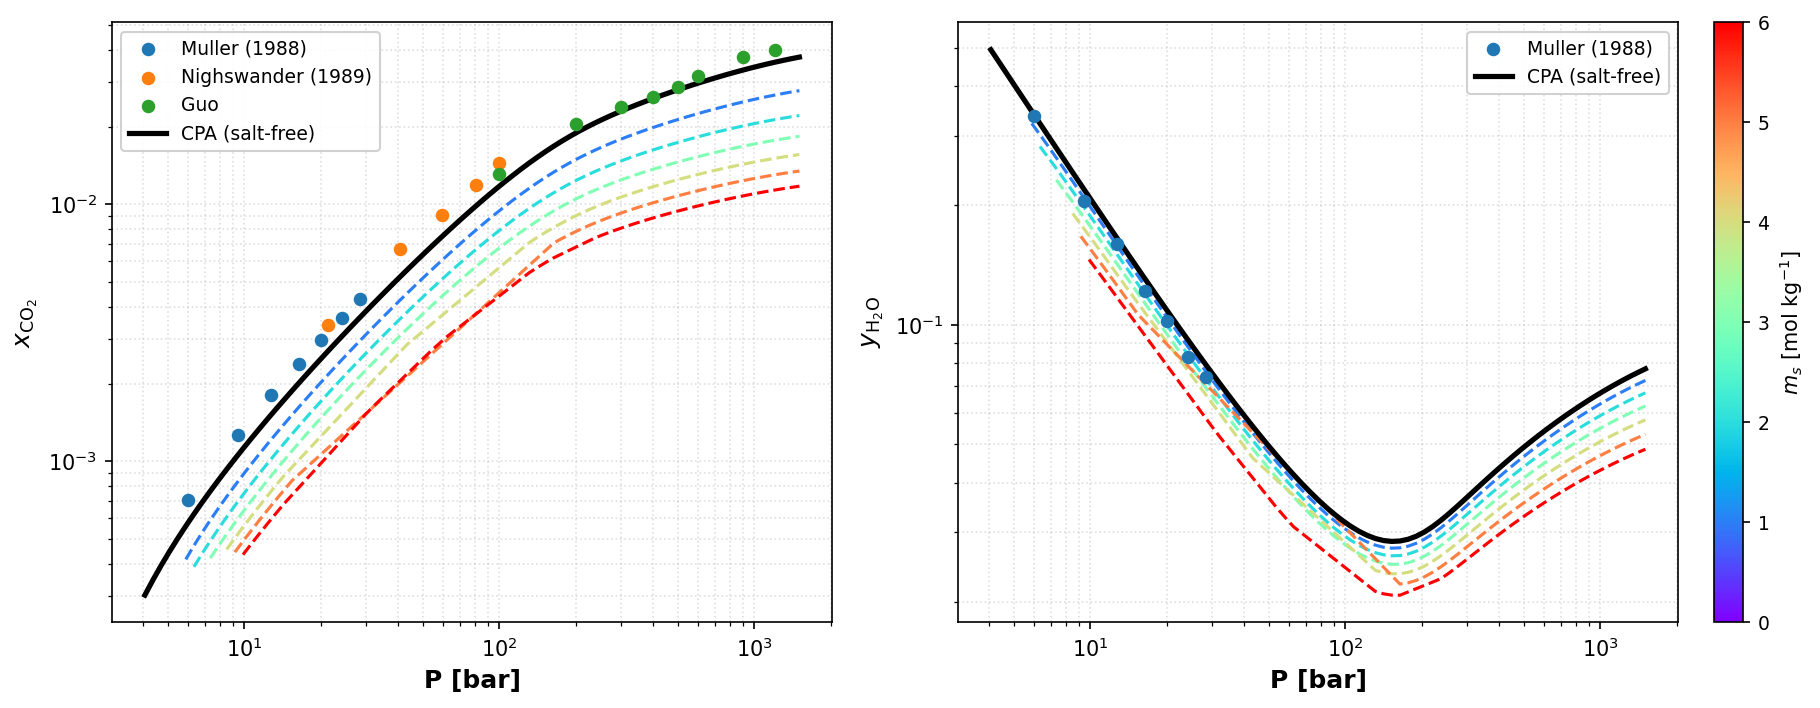
\includegraphics[width=\textwidth]{../figures/co2h2o/T393K.png}\caption{393\,K}\end{subfigure}\hfill
  \begin{subfigure}[t]{\swsi}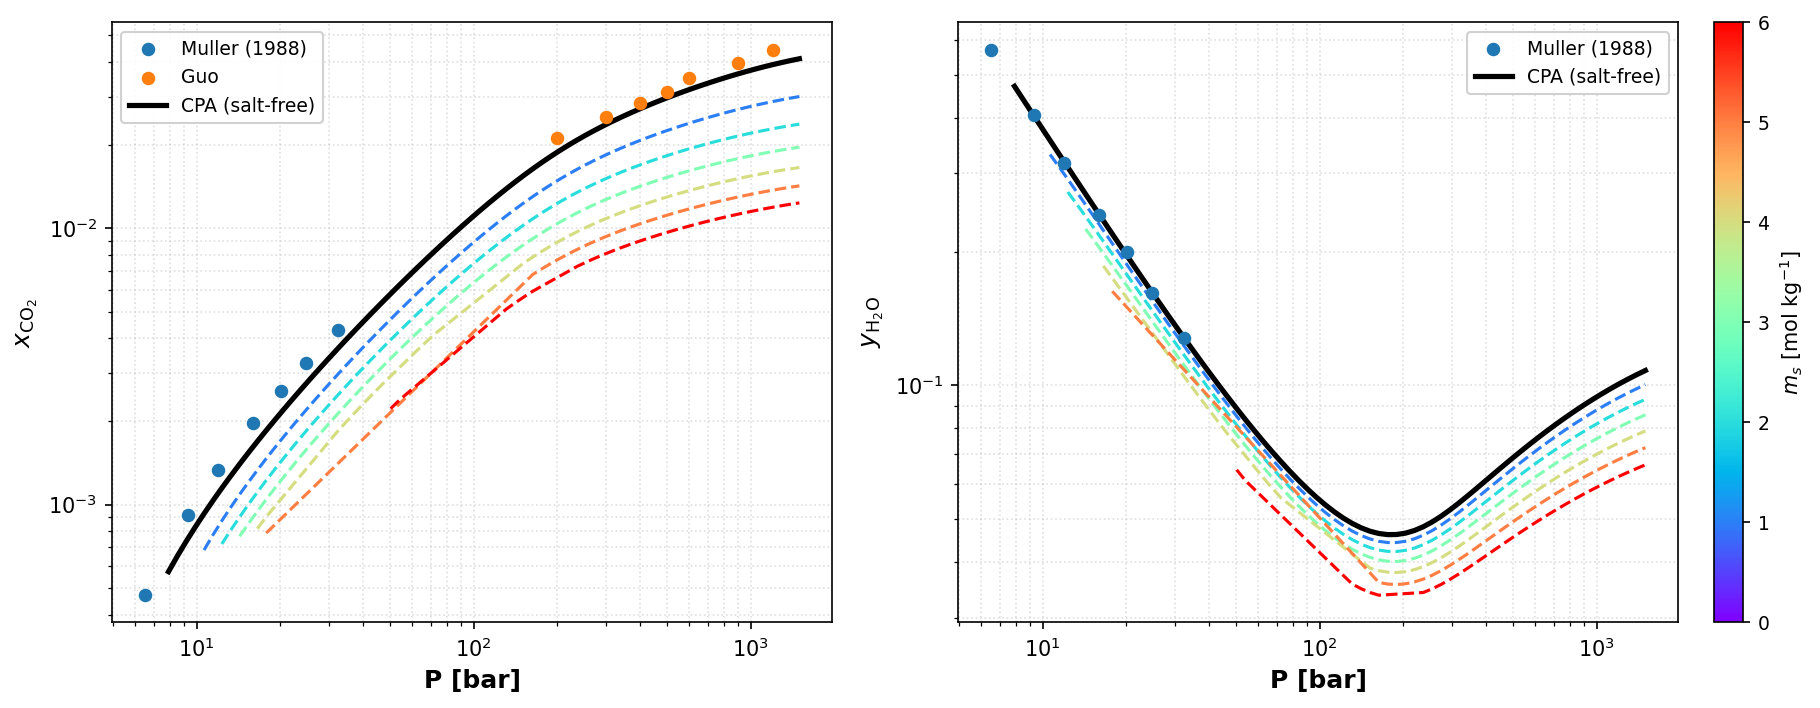
\includegraphics[width=\textwidth]{../figures/co2h2o/T413K.png}\caption{413\,K}\end{subfigure}\hfill
  \begin{subfigure}[t]{\swsi}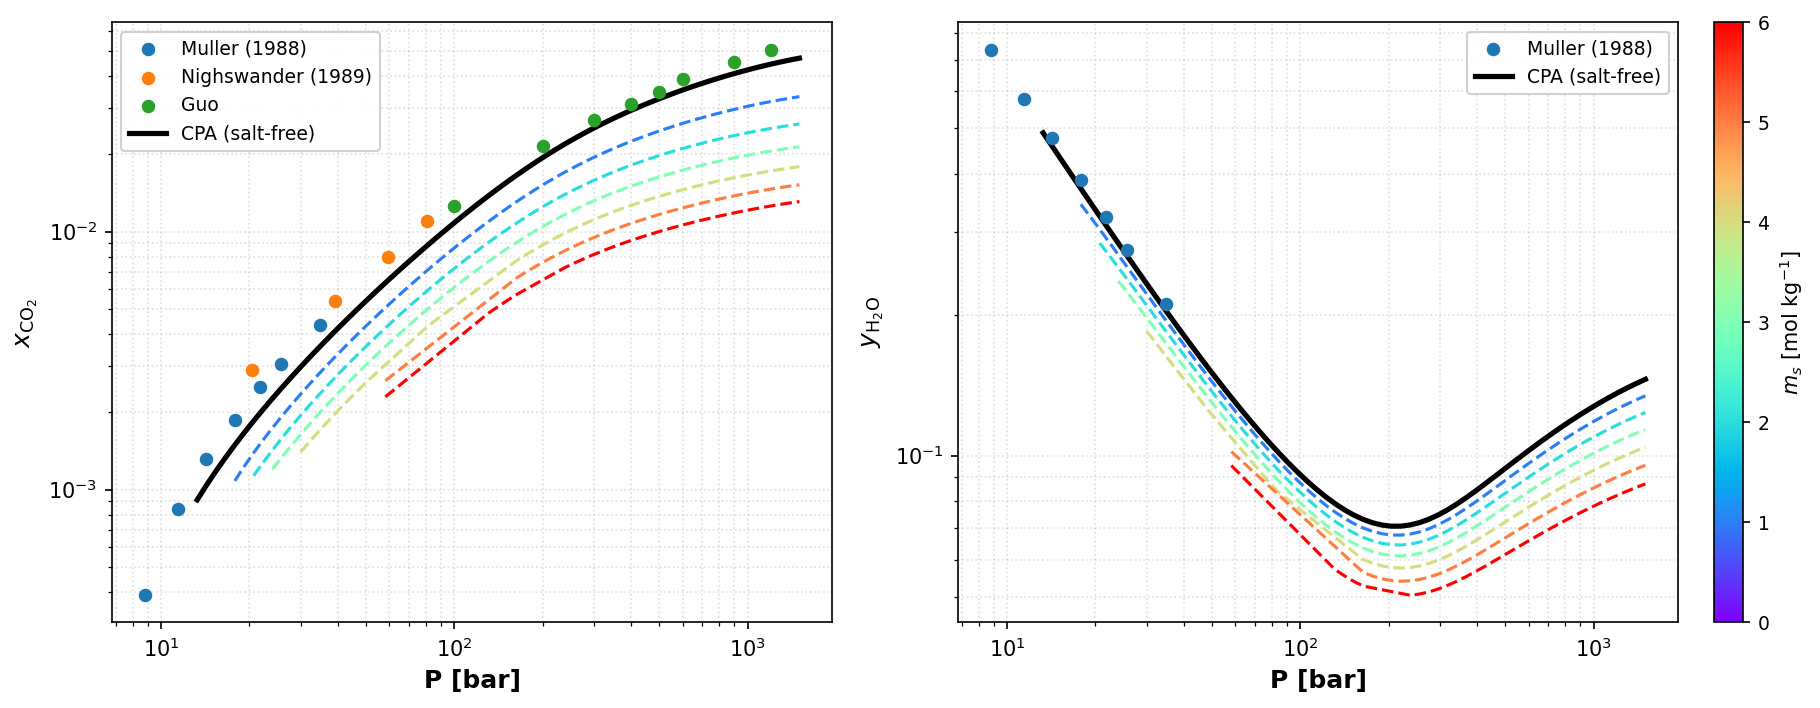
\includegraphics[width=\textwidth]{../figures/co2h2o/T433K.png}\caption{433\,K}\end{subfigure}\\[4pt]
  \begin{subfigure}[t]{\swsi}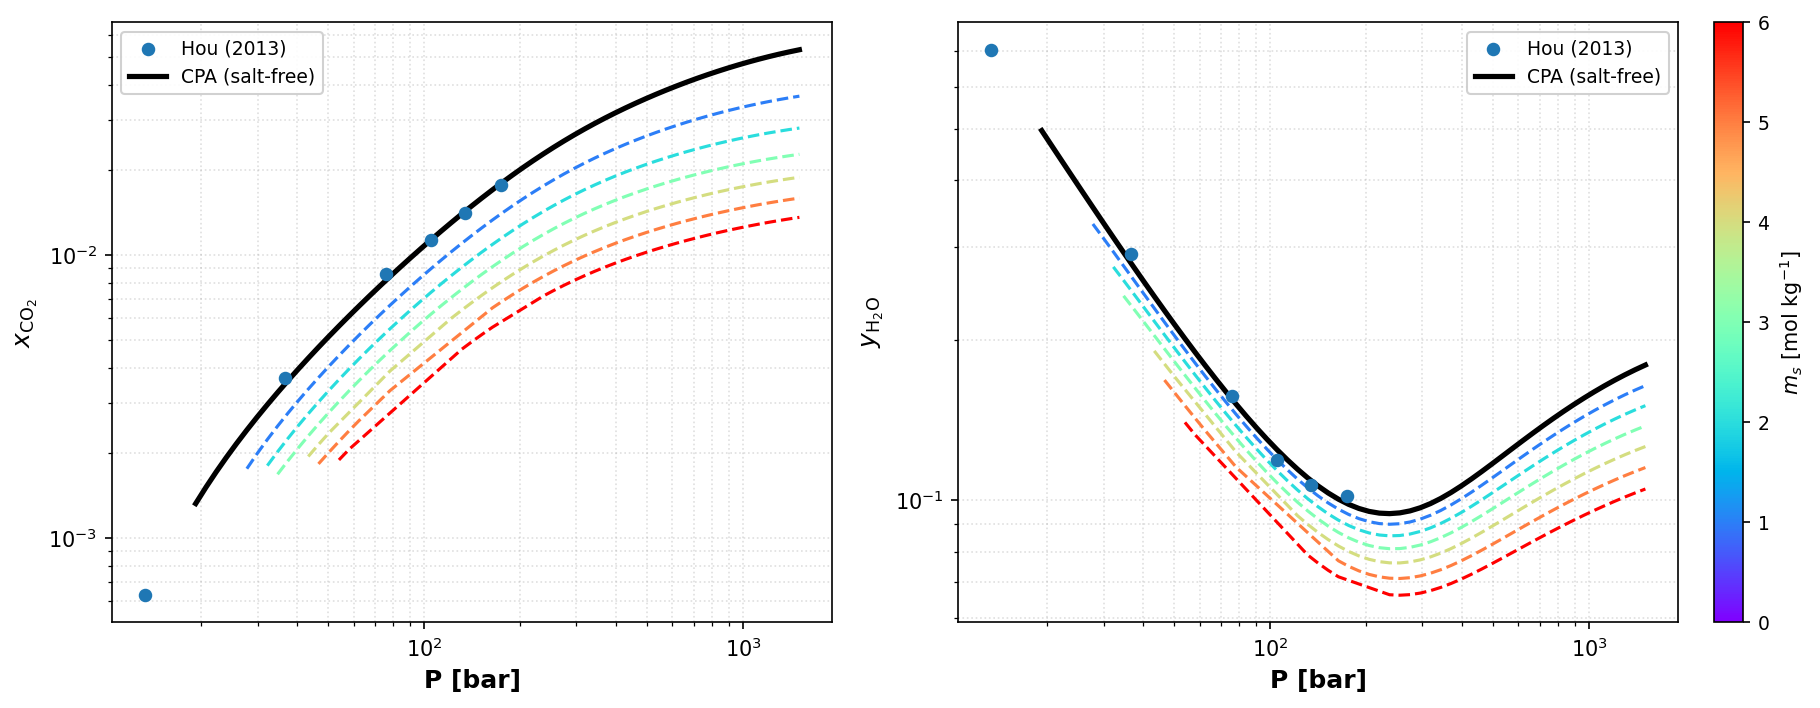
\includegraphics[width=\textwidth]{../figures/co2h2o/T448K.png}\caption{448\,K}\end{subfigure}\hfill
  \begin{subfigure}[t]{\swsi}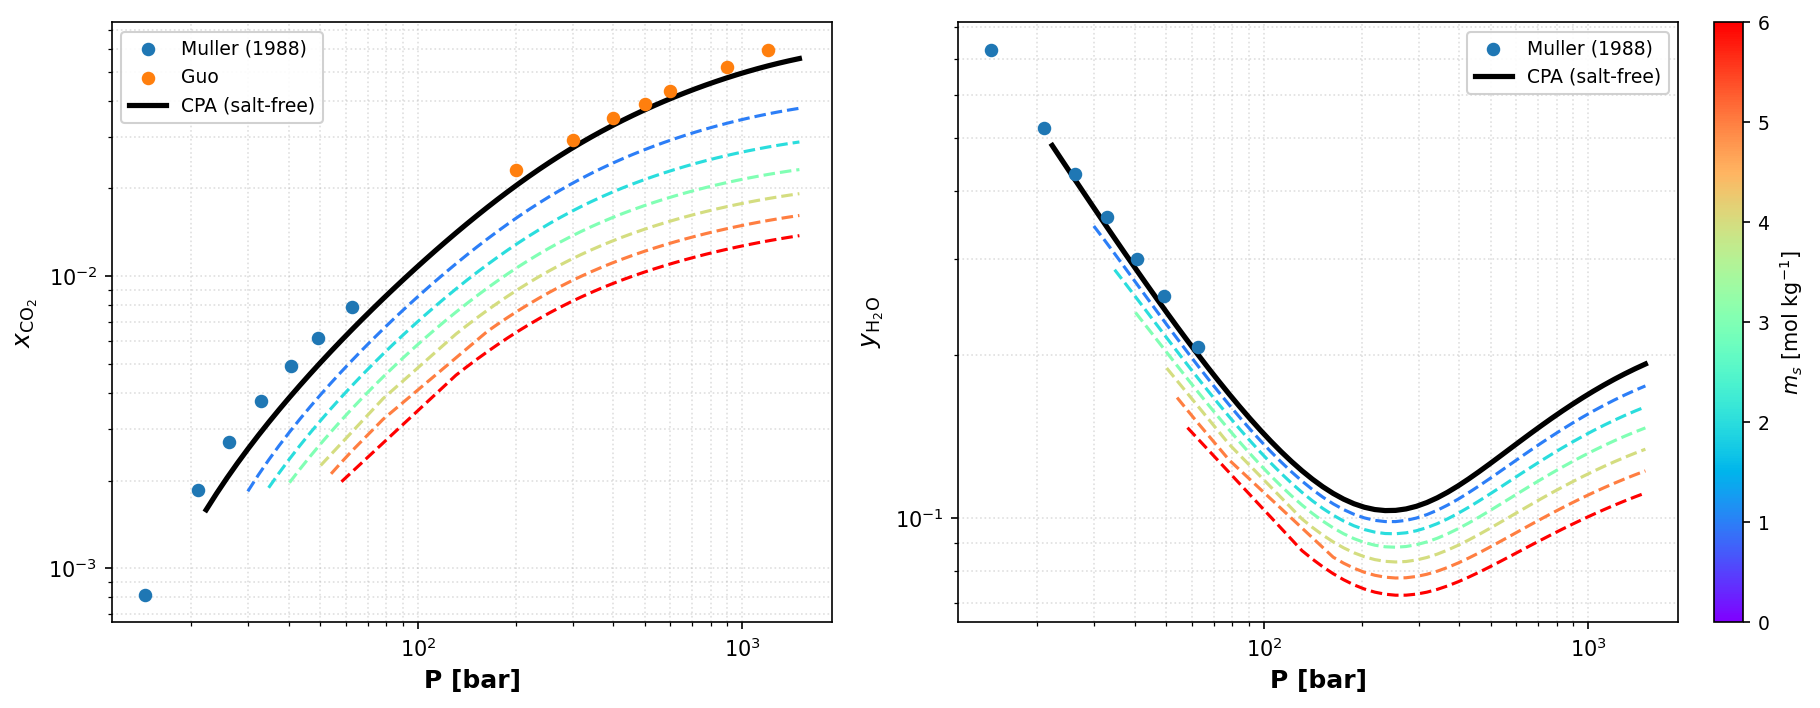
\includegraphics[width=\textwidth]{../figures/co2h2o/T453K.png}\caption{453\,K}\end{subfigure}\hfill
  \begin{subfigure}[t]{\swsi}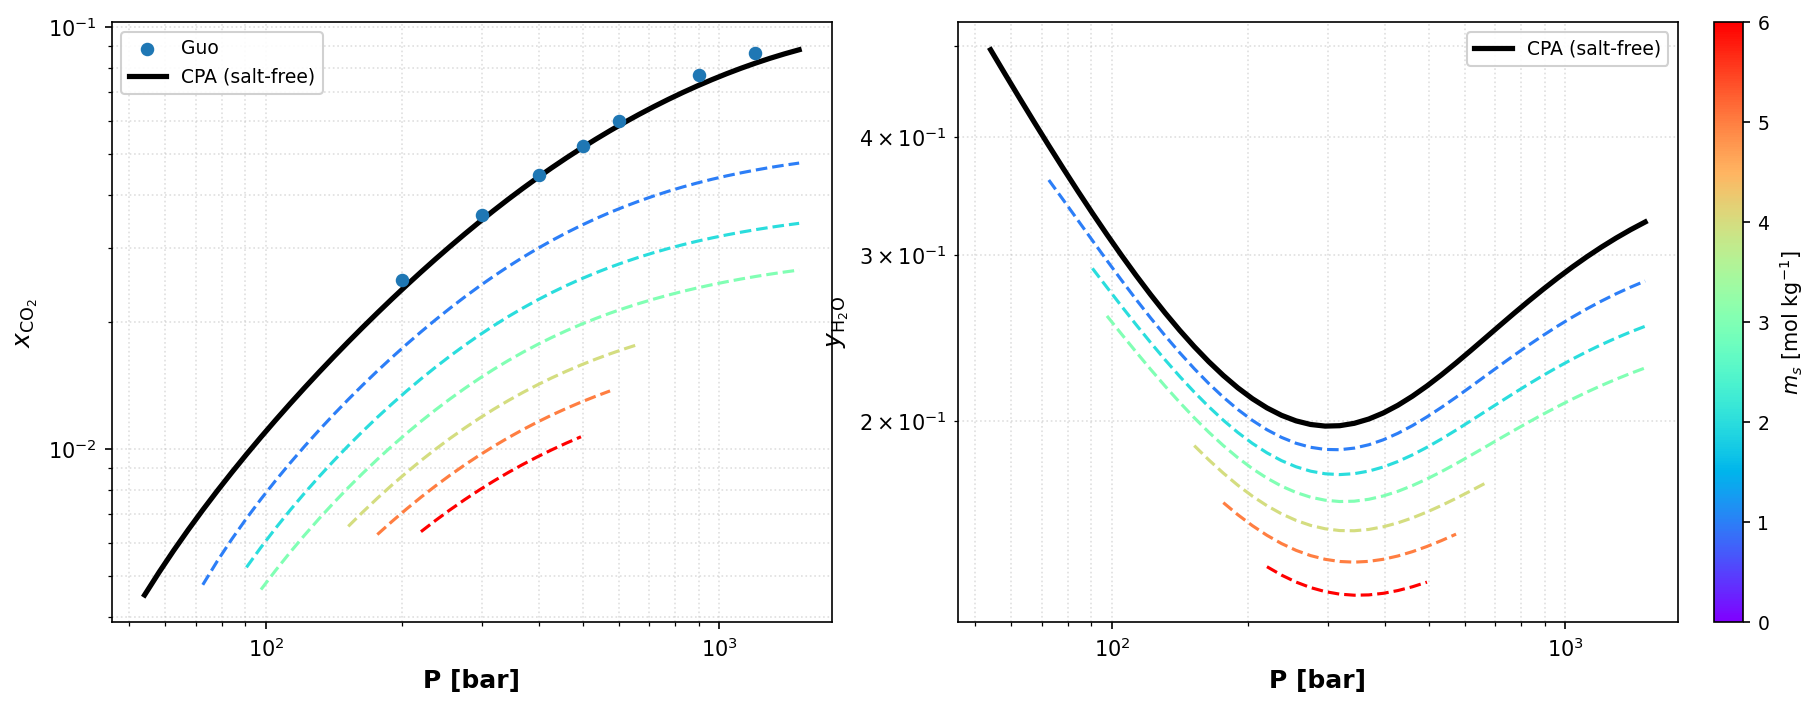
\includegraphics[width=\textwidth]{../figures/co2h2o/T493K.png}\caption{493\,K}\end{subfigure}\hfill
  \begin{subfigure}[t]{\swsi}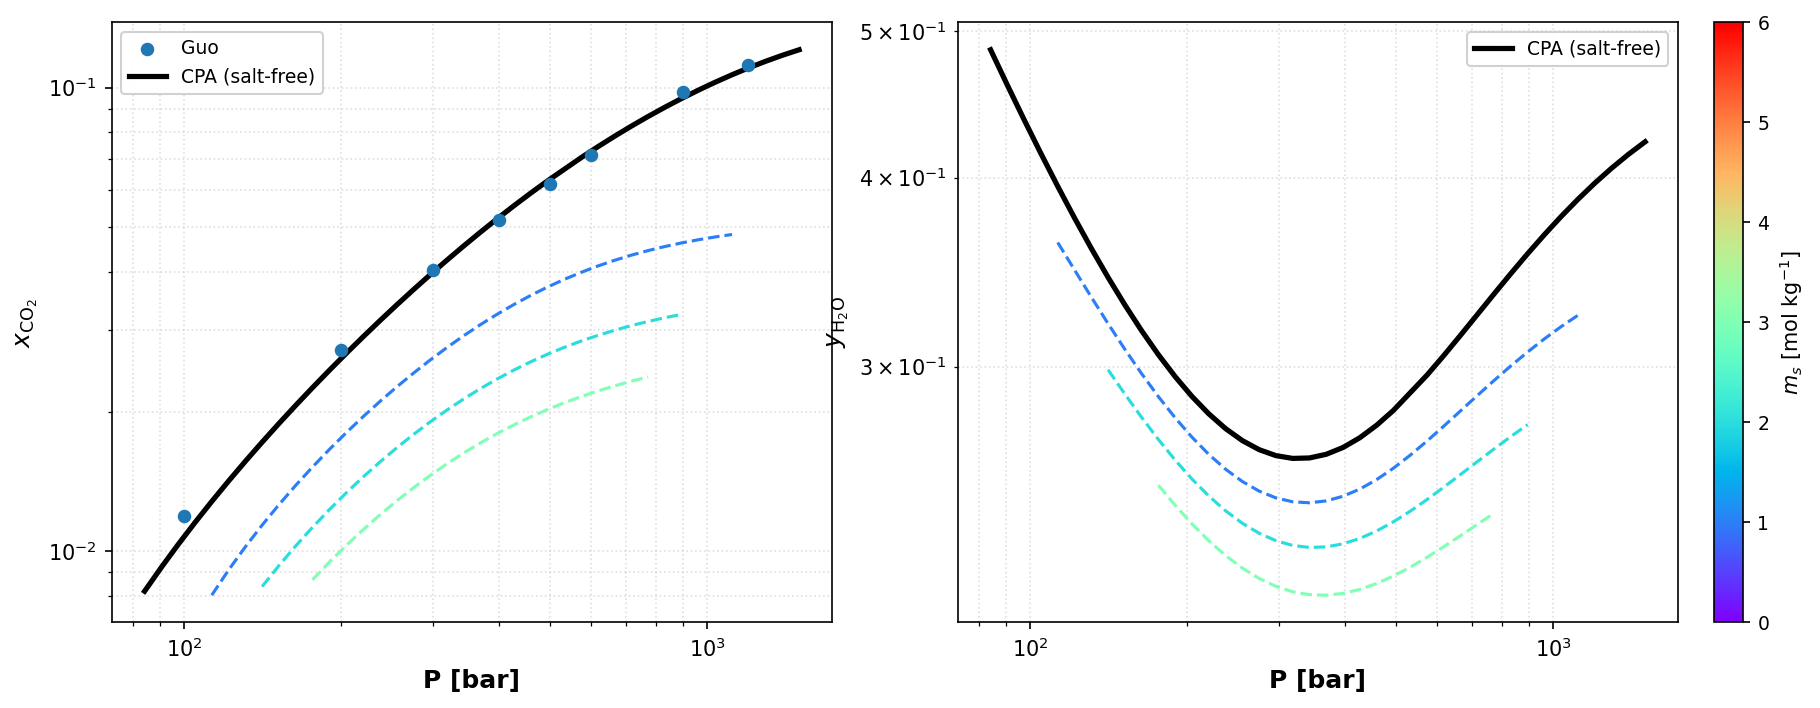
\includegraphics[width=\textwidth]{../figures/co2h2o/T513K.png}\caption{513\,K}\end{subfigure}\\[4pt]
  \begin{subfigure}[t]{\swsi}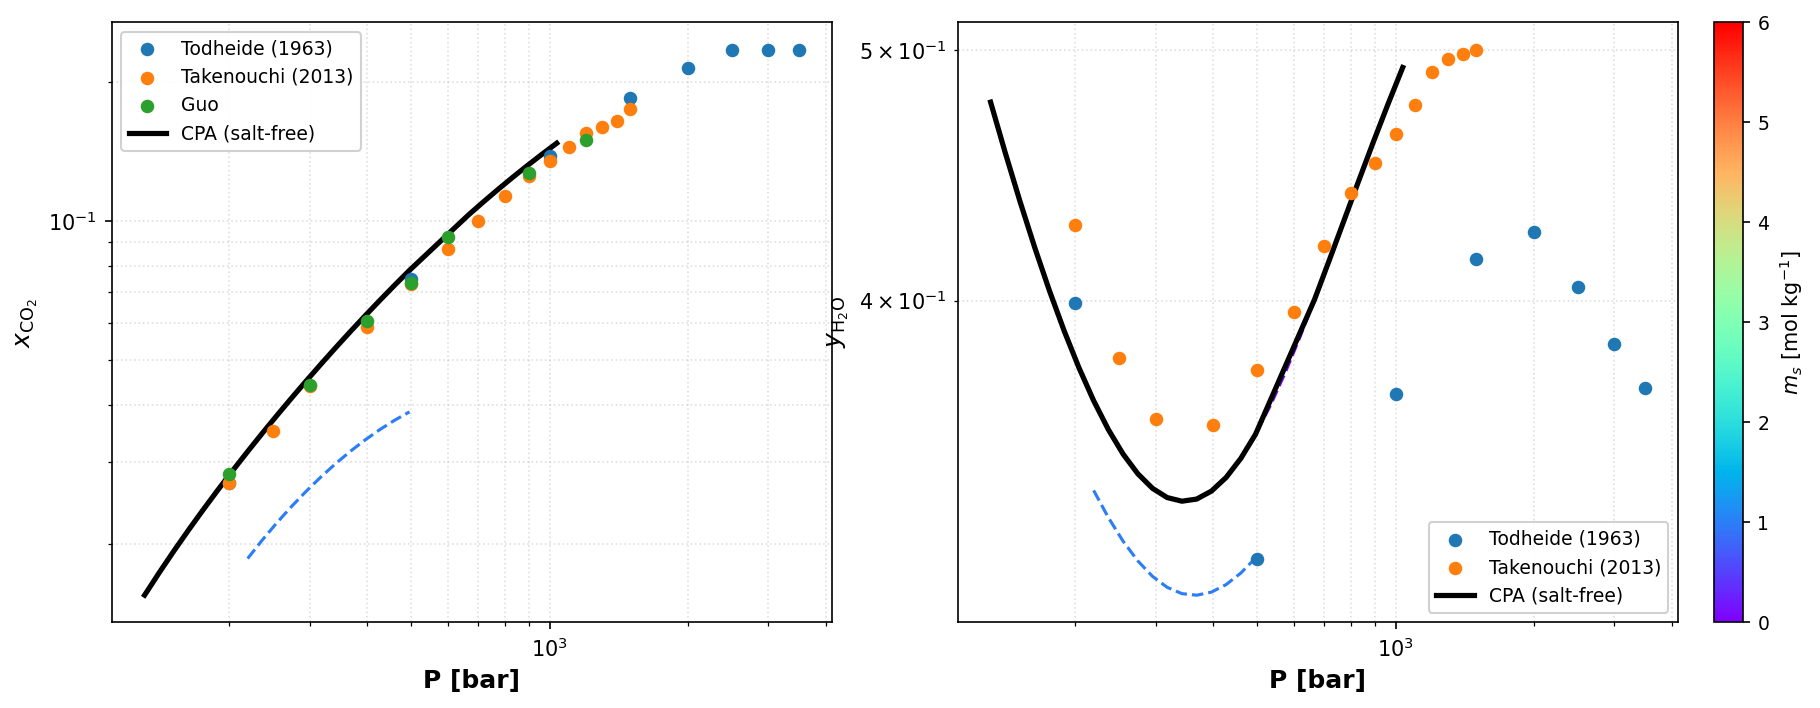
\includegraphics[width=\textwidth]{../figures/co2h2o/T533K.png}\caption{533\,K}\end{subfigure}\hfill
  \begin{subfigure}[t]{\swsi}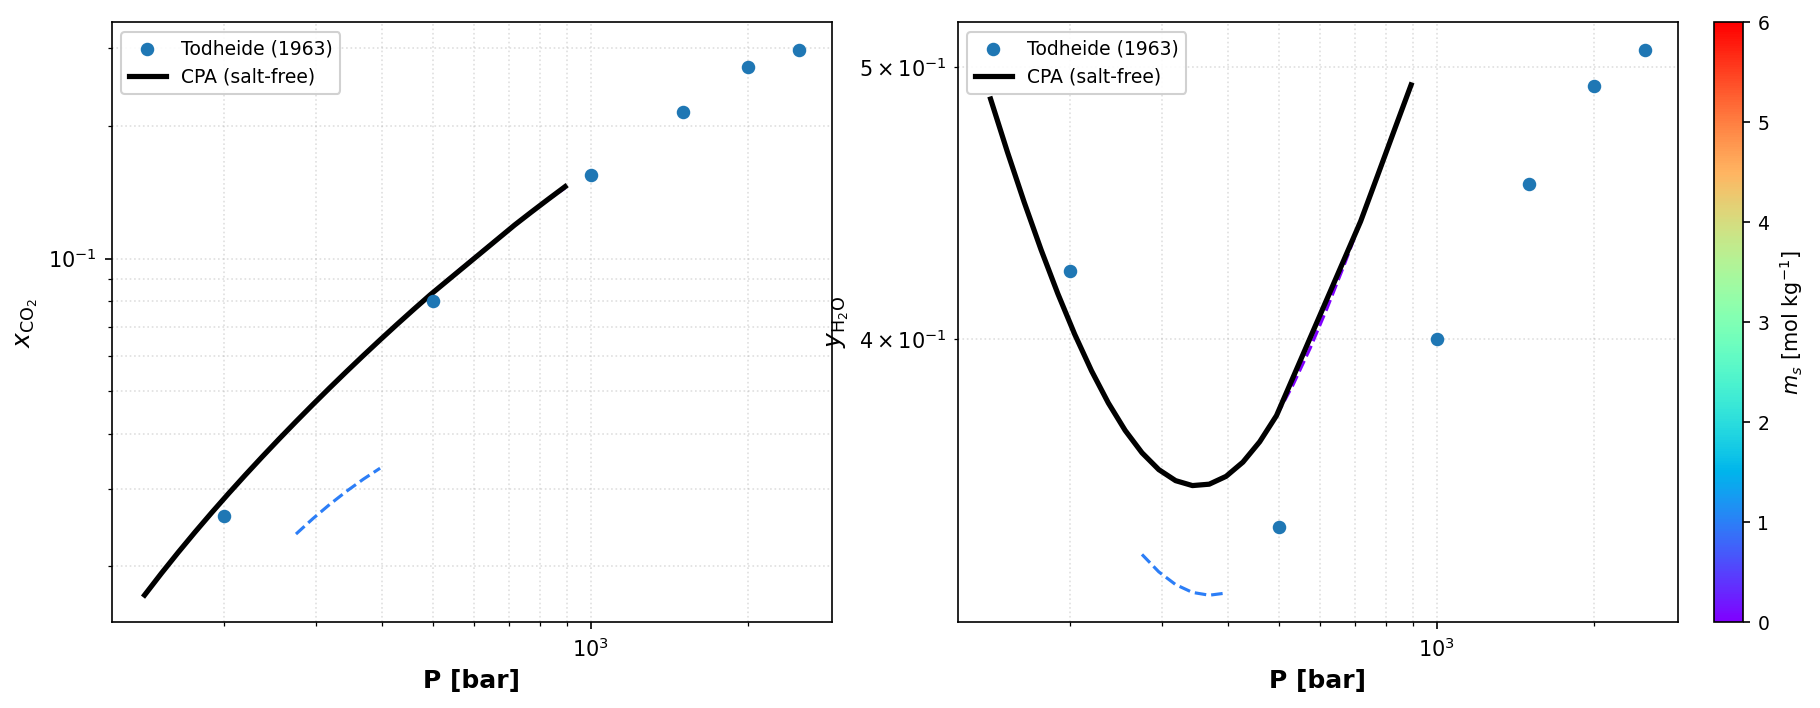
\includegraphics[width=\textwidth]{../figures/co2h2o/T538K.png}\caption{538\,K}\end{subfigure}\hfill
  \begin{subfigure}[t]{\swsi}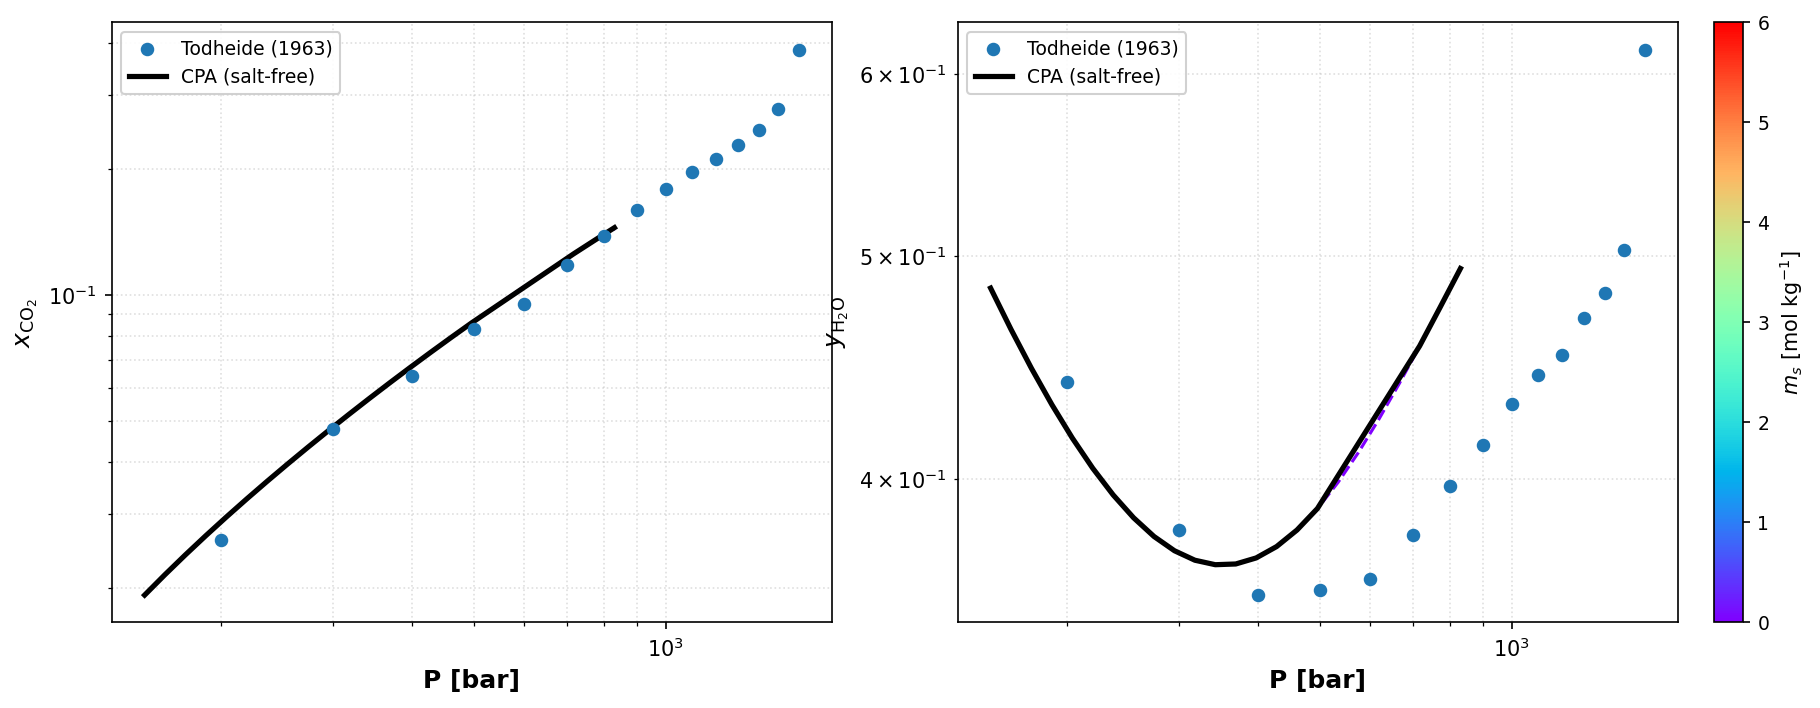
\includegraphics[width=\textwidth]{../figures/co2h2o/T541K.png}\caption{541\,K}\end{subfigure}\hfill
  \begin{subfigure}[t]{\swsi}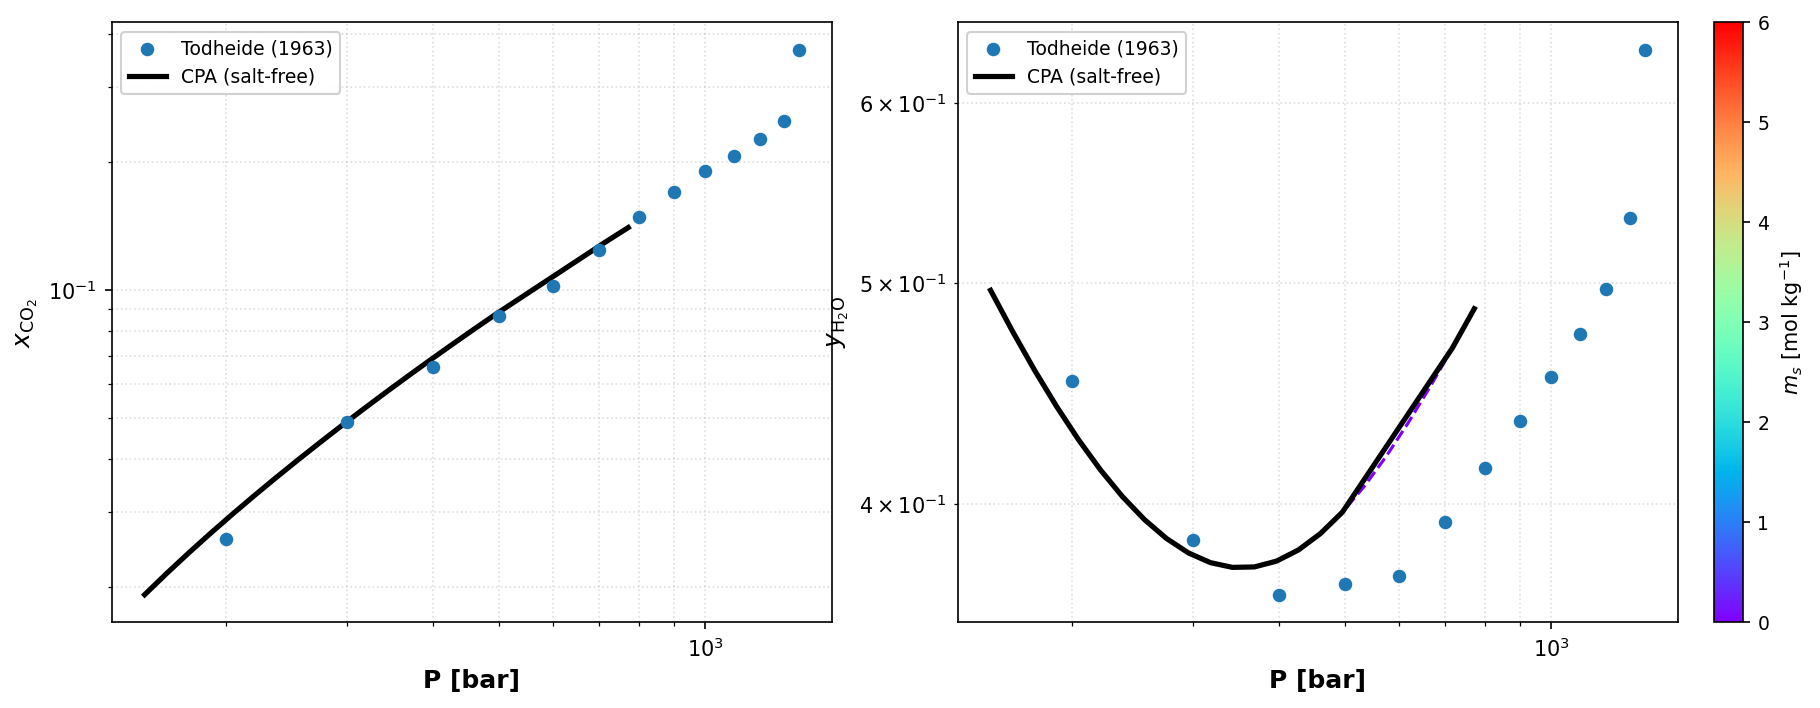
\includegraphics[width=\textwidth]{../figures/co2h2o/T543K.png}\caption{543\,K}\end{subfigure}\\[4pt]
  \begin{subfigure}[t]{\swsi}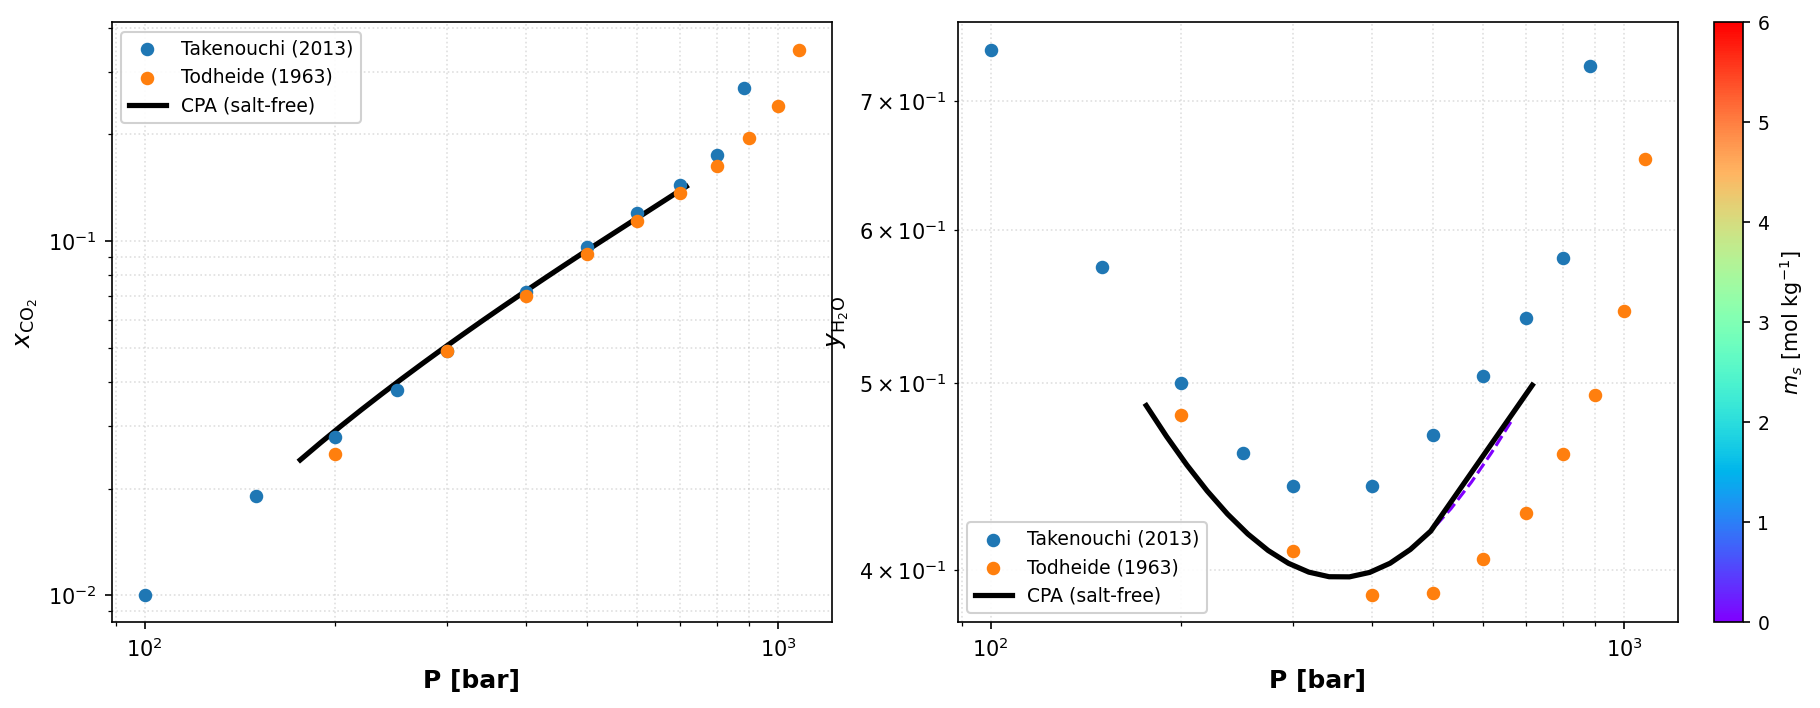
\includegraphics[width=\textwidth]{../figures/co2h2o/T548K.png}\caption{548\,K}\end{subfigure}\hfill
  \begin{subfigure}[t]{\swsi}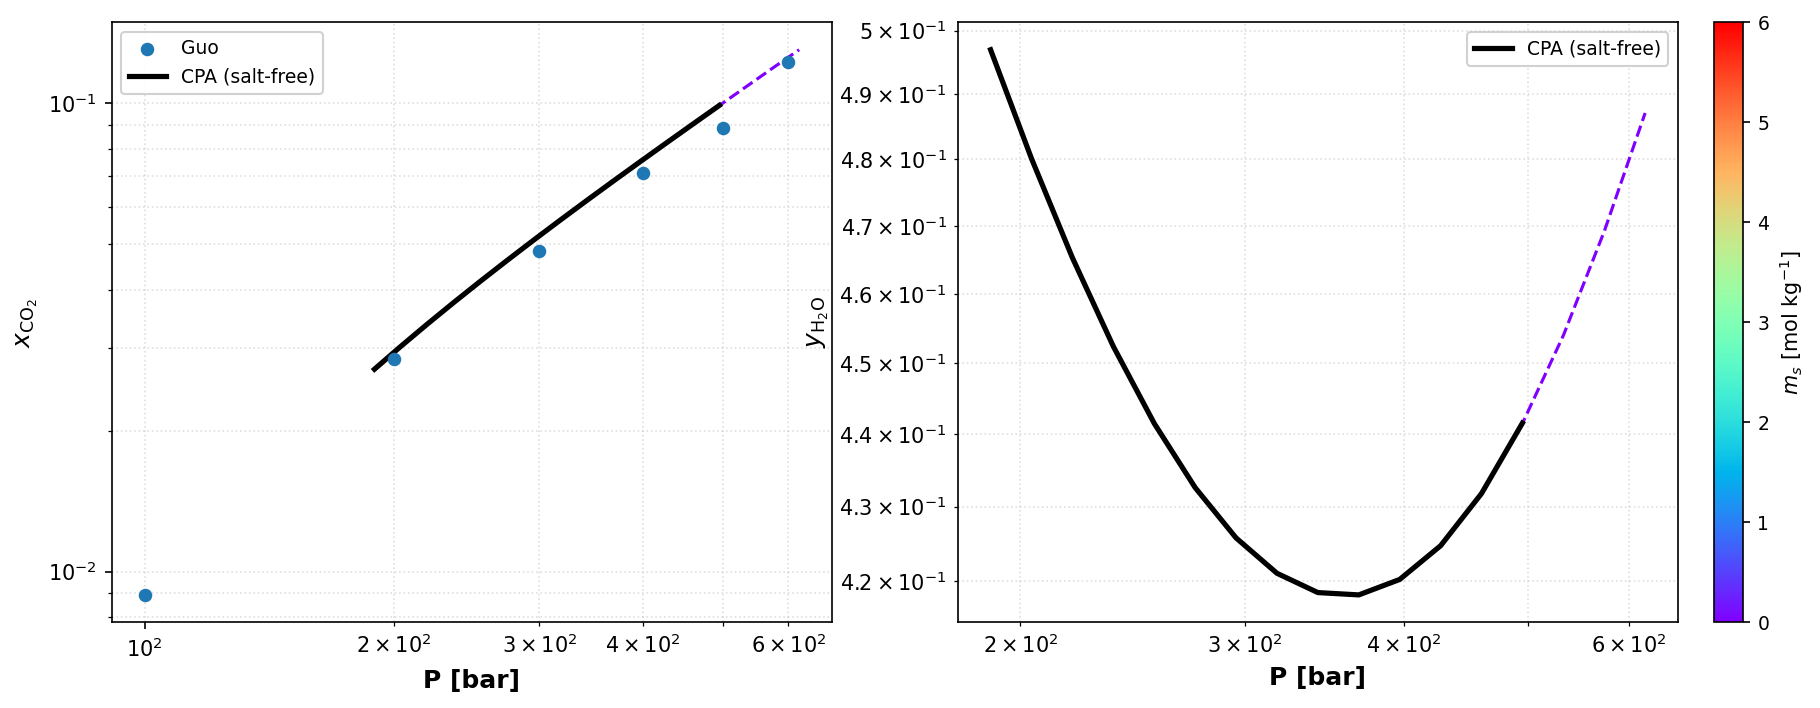
\includegraphics[width=\textwidth]{../figures/co2h2o/T553K.png}\caption{553\,K}\end{subfigure}\hfill
  \begin{subfigure}[t]{\swsi}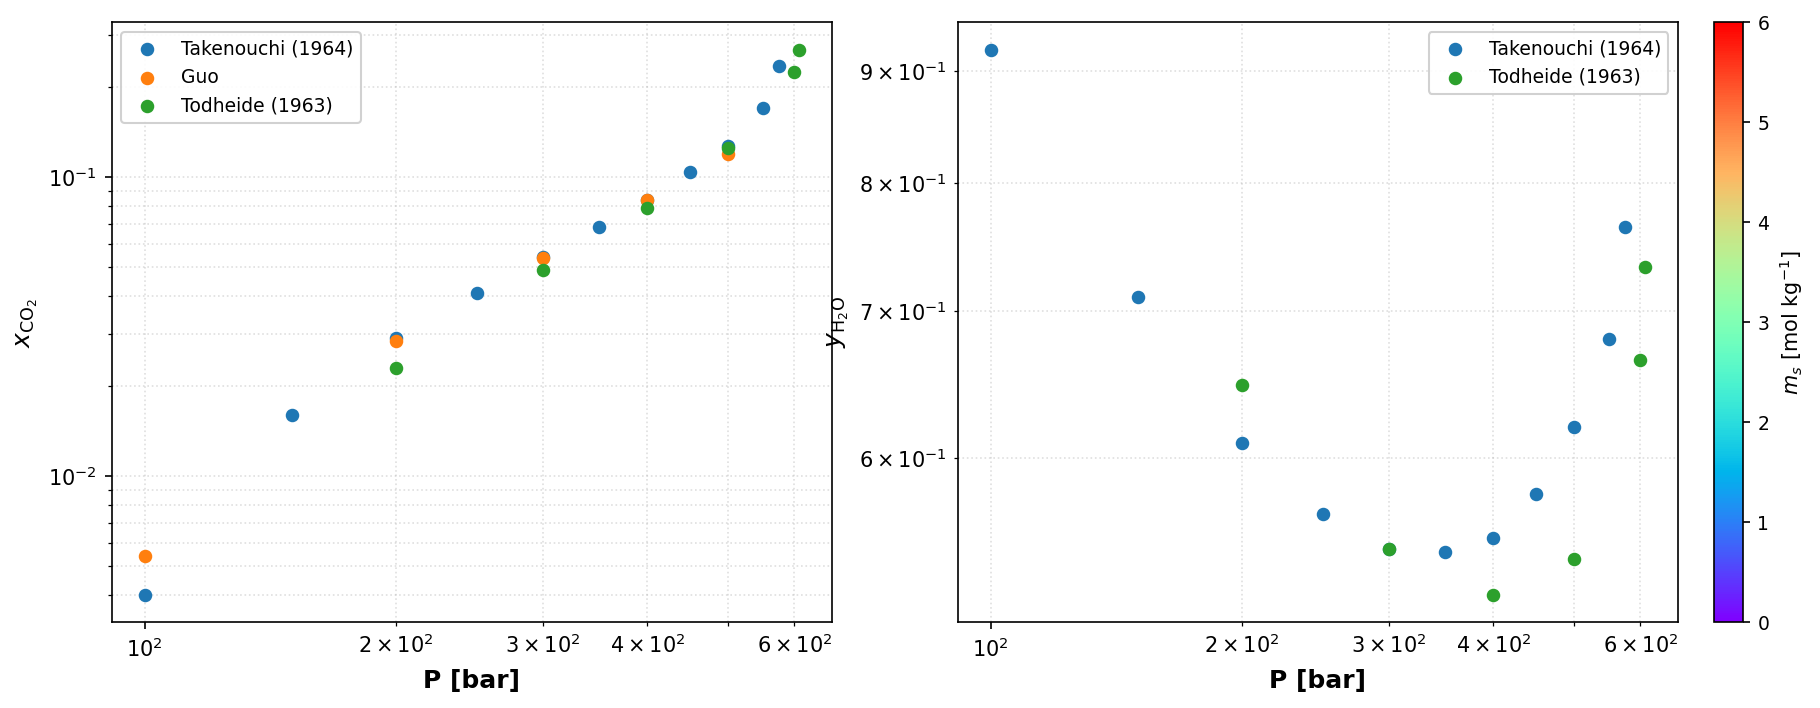
\includegraphics[width=\textwidth]{../figures/co2h2o/T573K.png}\caption{573\,K}\end{subfigure}\hfill
  \begin{subfigure}[t]{\swsi}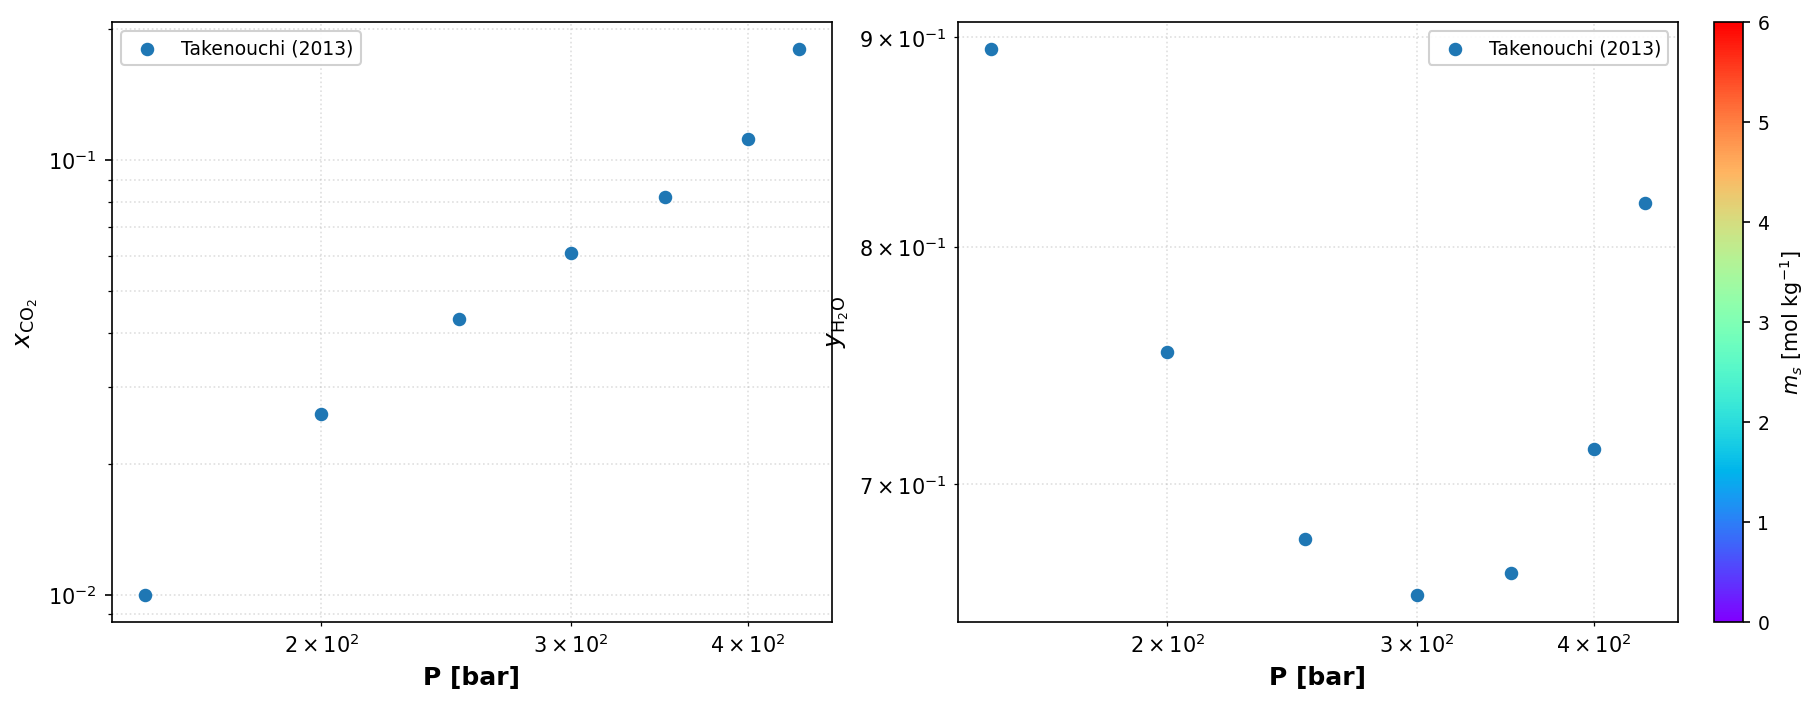
\includegraphics[width=\textwidth]{../figures/co2h2o/T598K.png}\caption{598\,K}\end{subfigure}\\[4pt]
  \begin{subfigure}[t]{\swsi}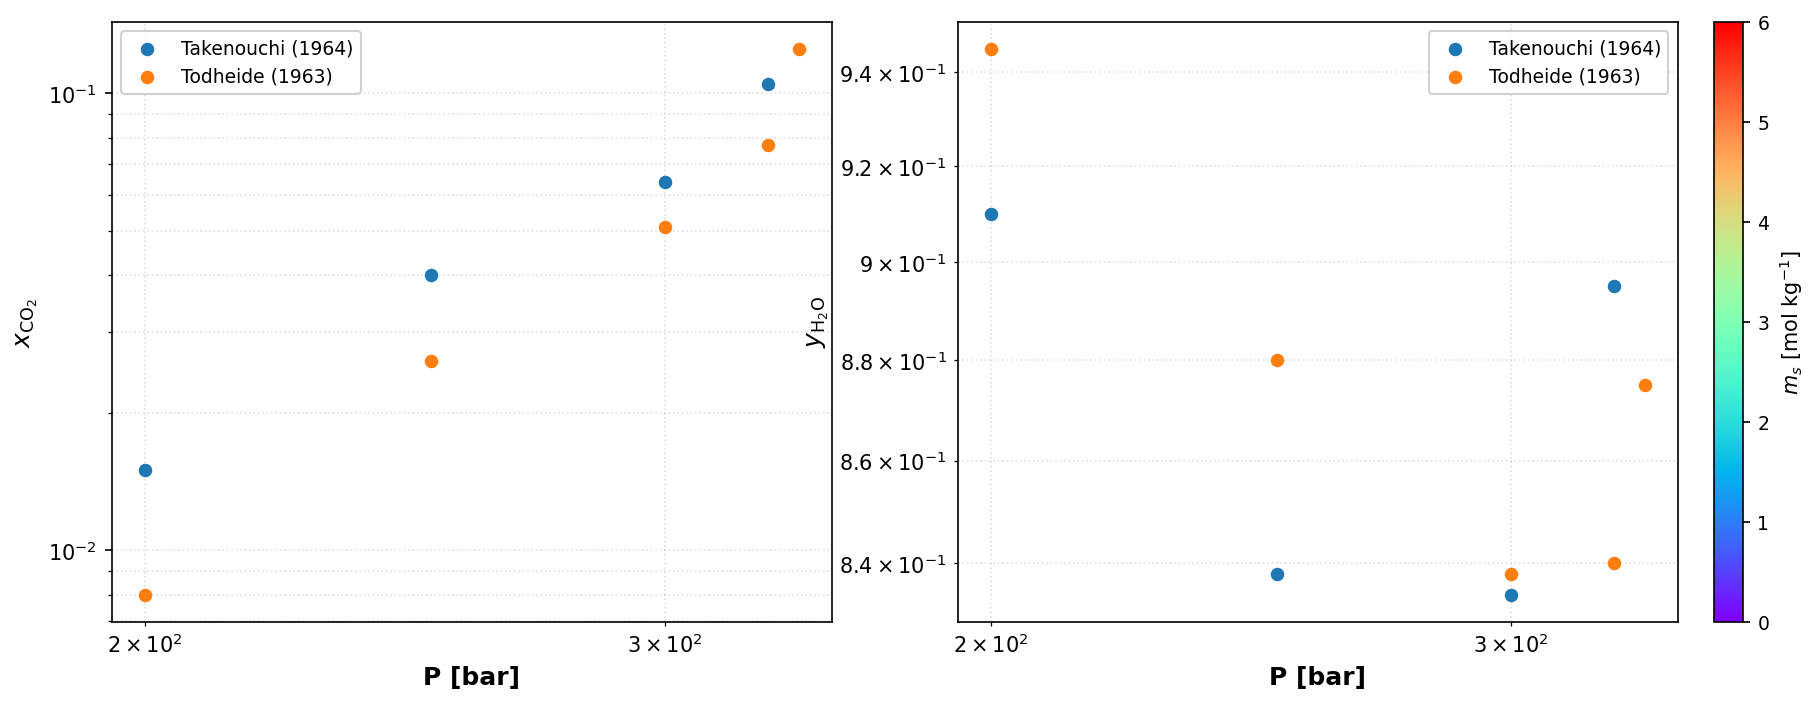
\includegraphics[width=\textwidth]{../figures/co2h2o/T623K.png}\caption{623\,K}\end{subfigure}\hfill
  \begin{subfigure}[t]{\swsi}\phantom{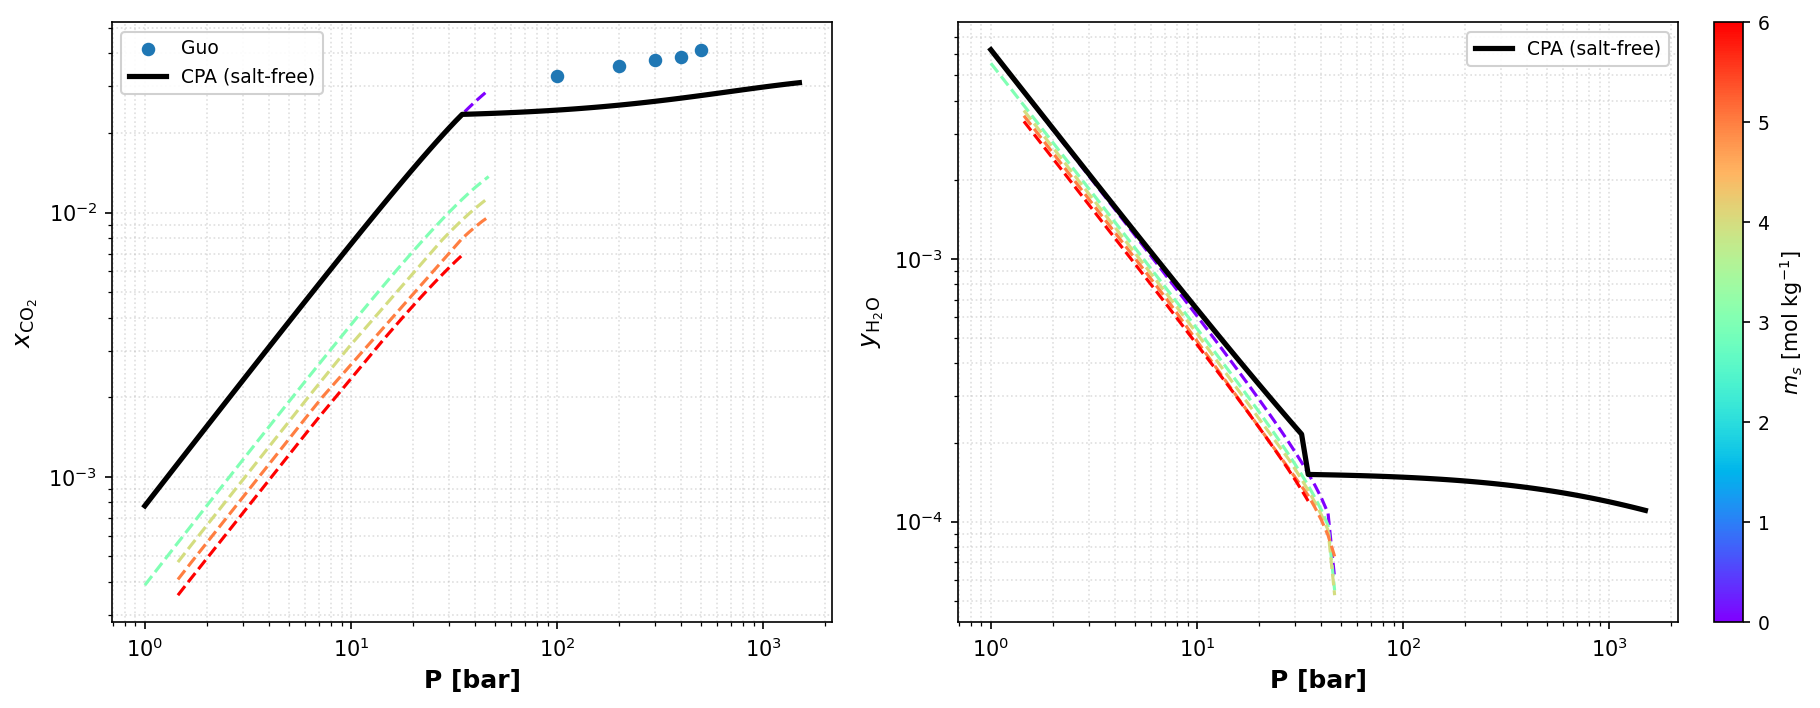
\includegraphics[width=\textwidth]{../figures/co2h2o/T273K.png}}\end{subfigure}\hfill
  \begin{subfigure}[t]{\swsi}\phantom{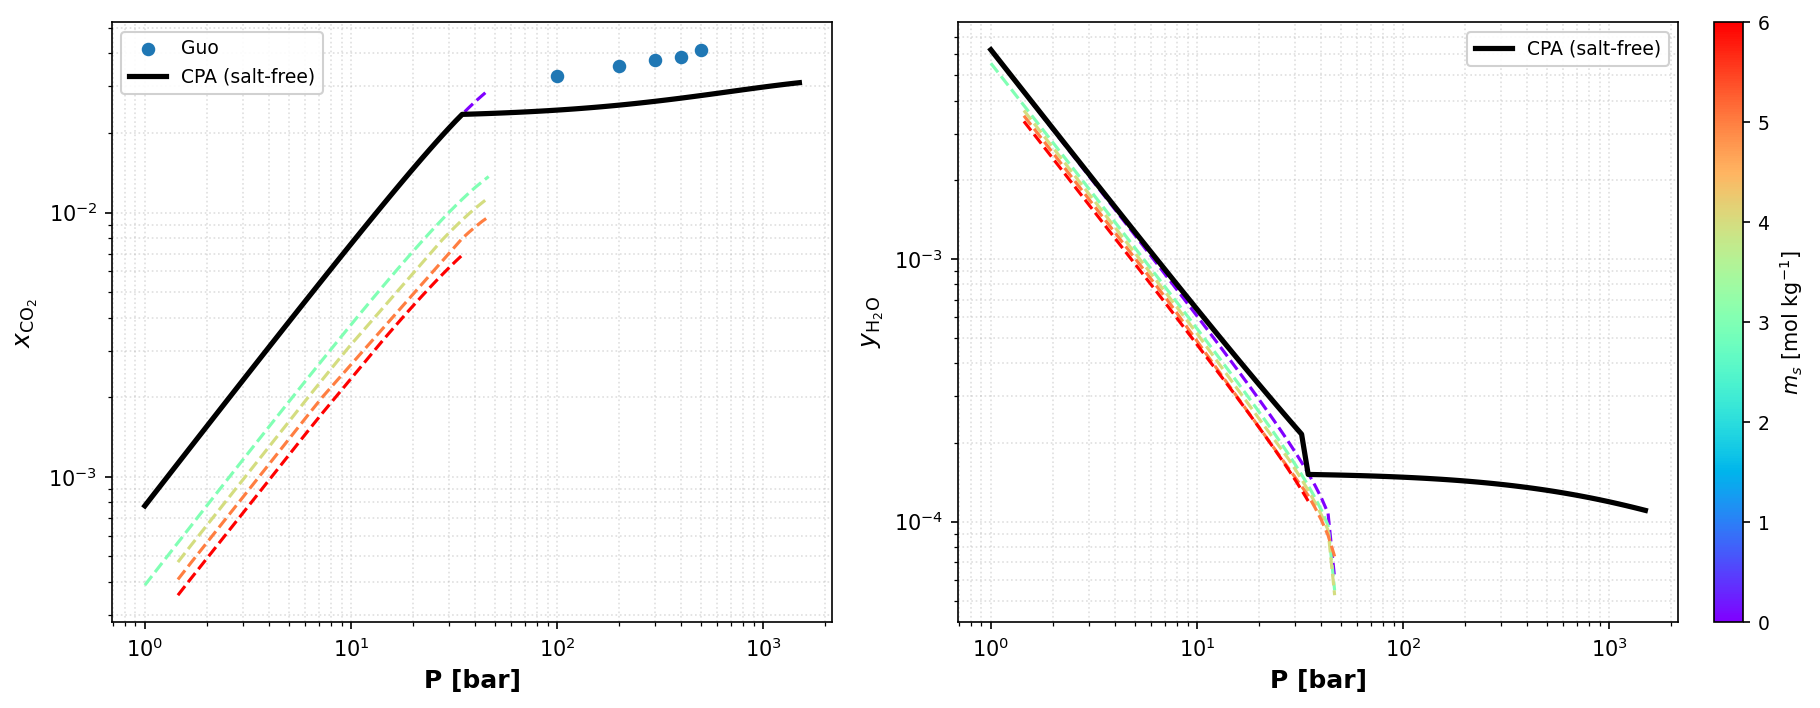
\includegraphics[width=\textwidth]{../figures/co2h2o/T273K.png}}\end{subfigure}\hfill
  \begin{subfigure}[t]{\swsi}\phantom{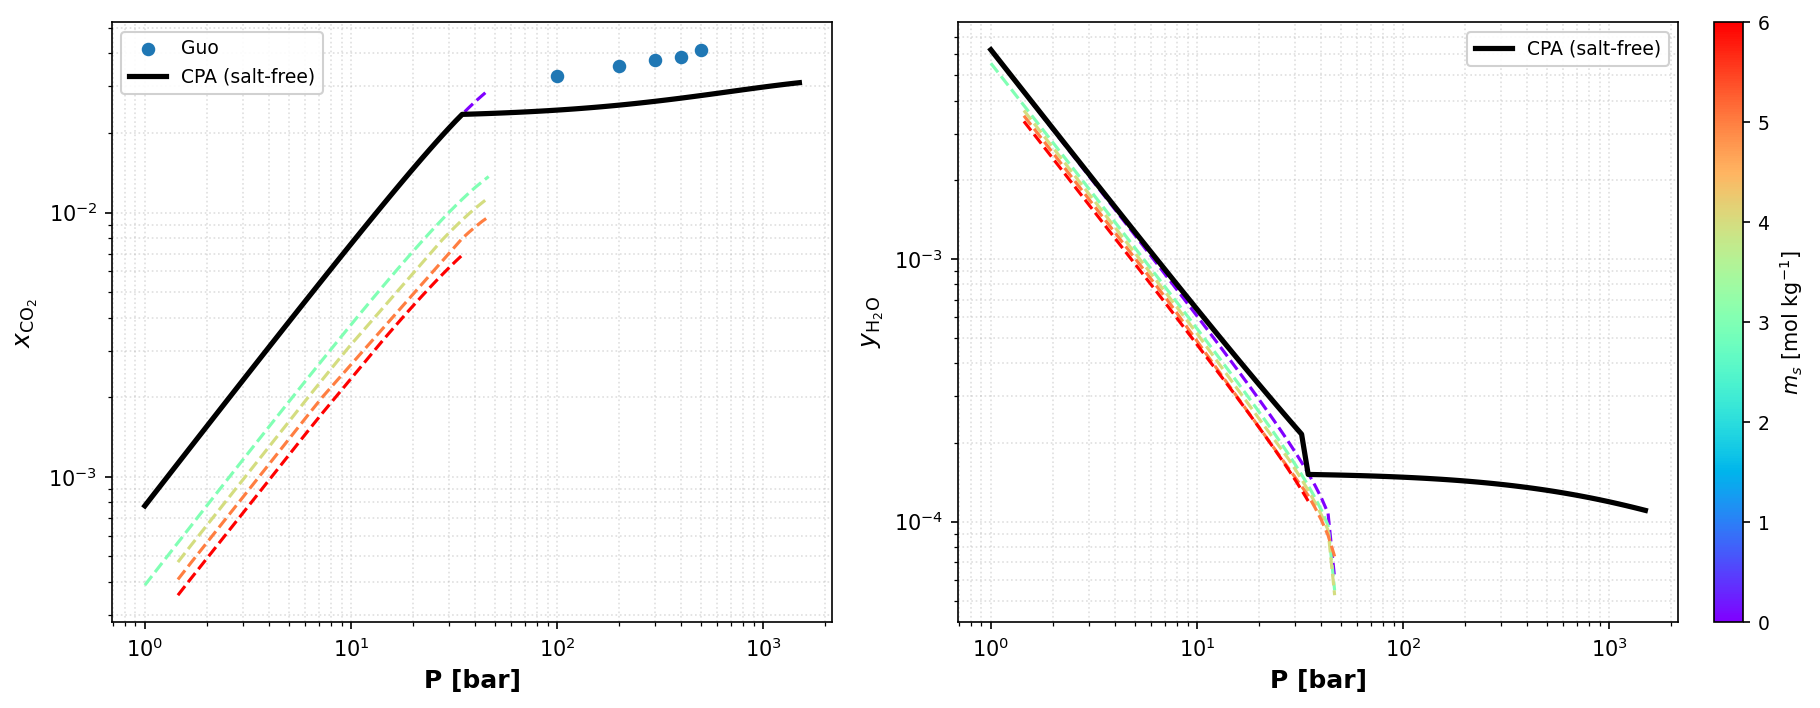
\includegraphics[width=\textwidth]{../figures/co2h2o/T273K.png}}\end{subfigure}
  \caption{CO$_2$ + H$_2$O phase equilibria at all 29 temperatures not shown in Fig.~\ref{fig:co2h2o_Tpanel}
           (273--623\,K), 4 panels per row.
           Each panel shows the CO$_2$ mole fraction in the aqueous phase ($x_{\text{CO}_2}$, left sub-panel)
           and H$_2$O mole fraction in the CO$_2$-rich phase ($y_{\text{H}_2\text{O}}$, right sub-panel) vs.\ pressure.
           Open symbols: experimental data \citep{Coelho2025}; black solid line: CPA (salt-free);
           dashed rainbow lines: eCPA at $m_s = 0$--$6$\,mol\,kg$^{-1}$ (violet to red).}
  \label{fig:co2h2o_Tpanel_SI}
\end{figure}

%% --- SI Figure S2: remaining single-panel CO2+NaCl panels ---
\begin{figure}[p]
  \centering
  \newcommand{\snwsi}{0.30\textwidth}%
  \begin{subfigure}[t]{\snwsi}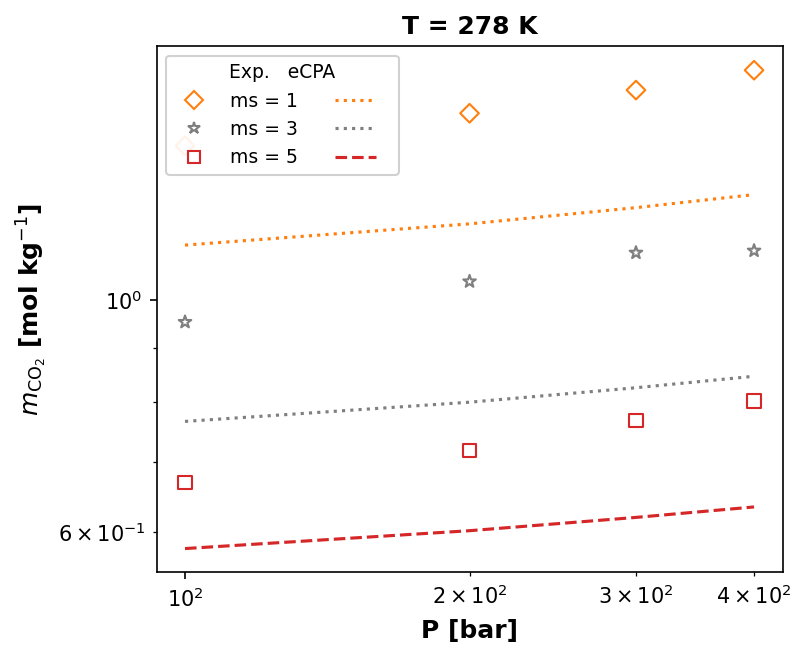
\includegraphics[width=\textwidth]{../figures/co2nacl/T278K.png}\caption{278\,K}\end{subfigure}\hfill
  \begin{subfigure}[t]{\snwsi}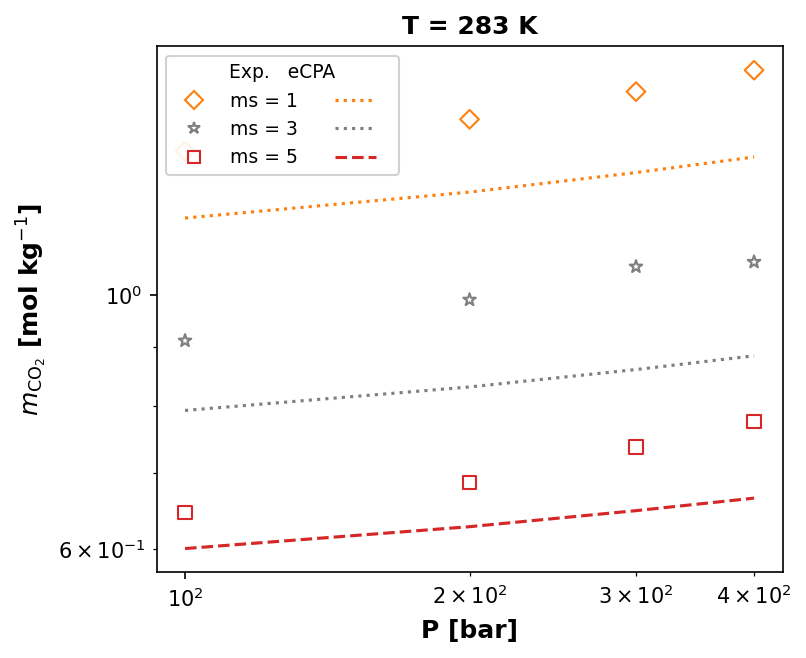
\includegraphics[width=\textwidth]{../figures/co2nacl/T283K.png}\caption{283\,K}\end{subfigure}\hfill
  \begin{subfigure}[t]{\snwsi}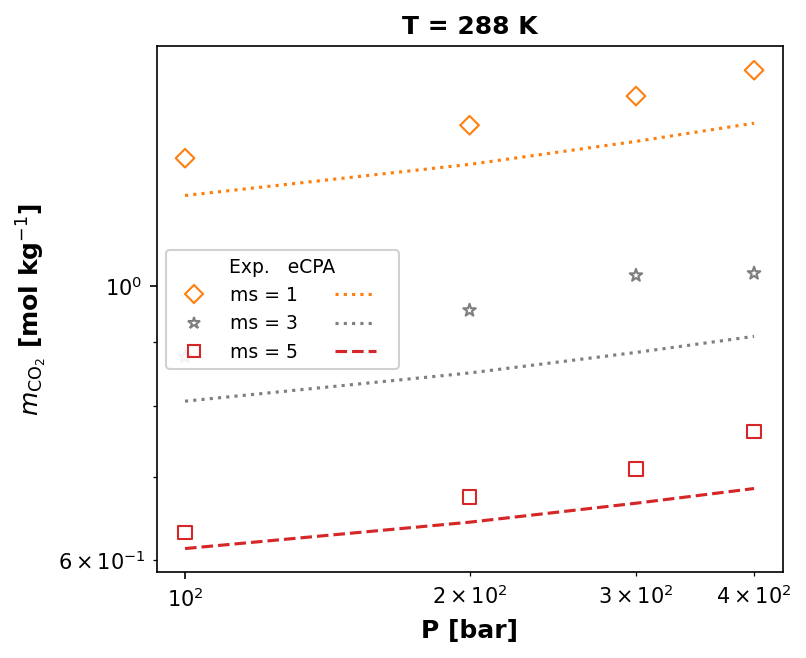
\includegraphics[width=\textwidth]{../figures/co2nacl/T288K.png}\caption{288\,K}\end{subfigure}\\[6pt]
  \begin{subfigure}[t]{\snwsi}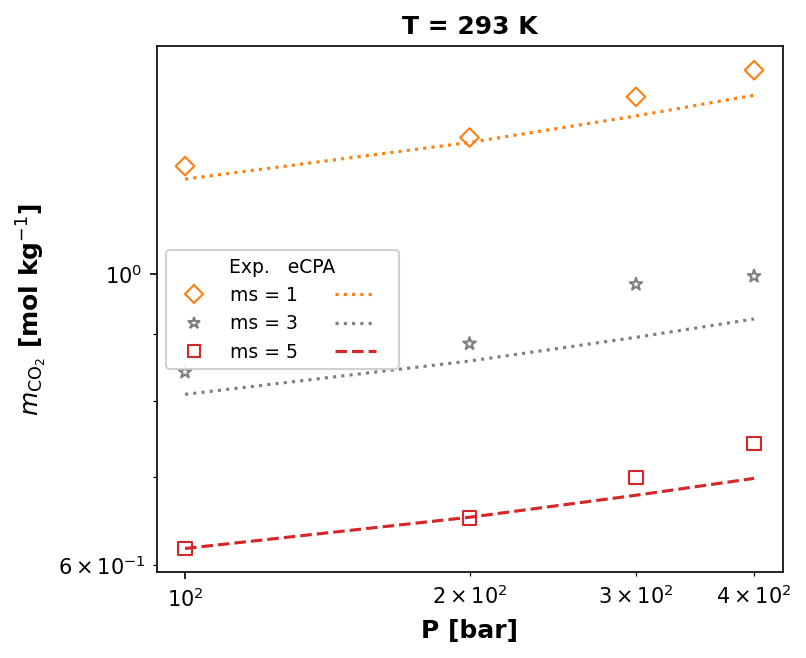
\includegraphics[width=\textwidth]{../figures/co2nacl/T293K.png}\caption{293\,K}\end{subfigure}\hfill
  \begin{subfigure}[t]{\snwsi}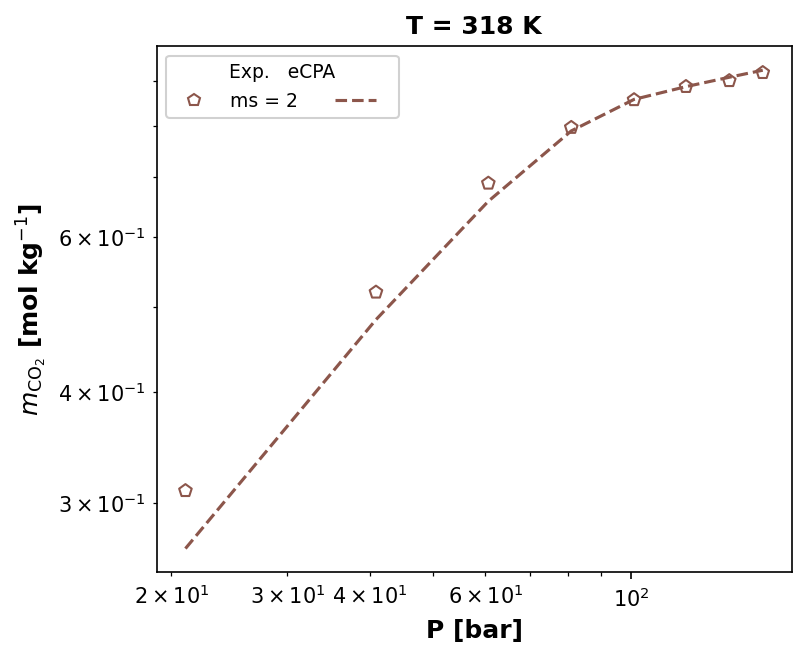
\includegraphics[width=\textwidth]{../figures/co2nacl/T318K.png}\caption{318\,K}\end{subfigure}\hfill
  \begin{subfigure}[t]{\snwsi}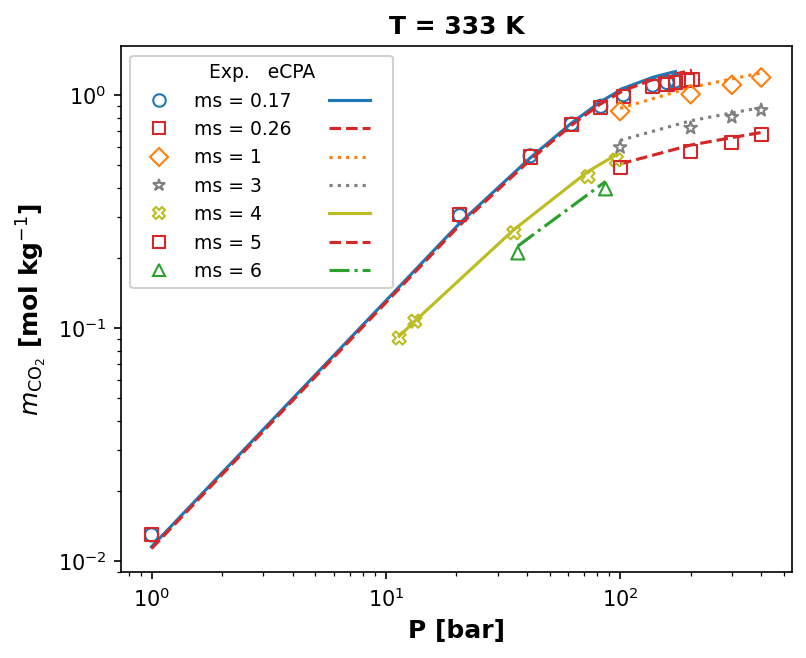
\includegraphics[width=\textwidth]{../figures/co2nacl/T333K.png}\caption{333\,K}\end{subfigure}\\[6pt]
  \begin{subfigure}[t]{\snwsi}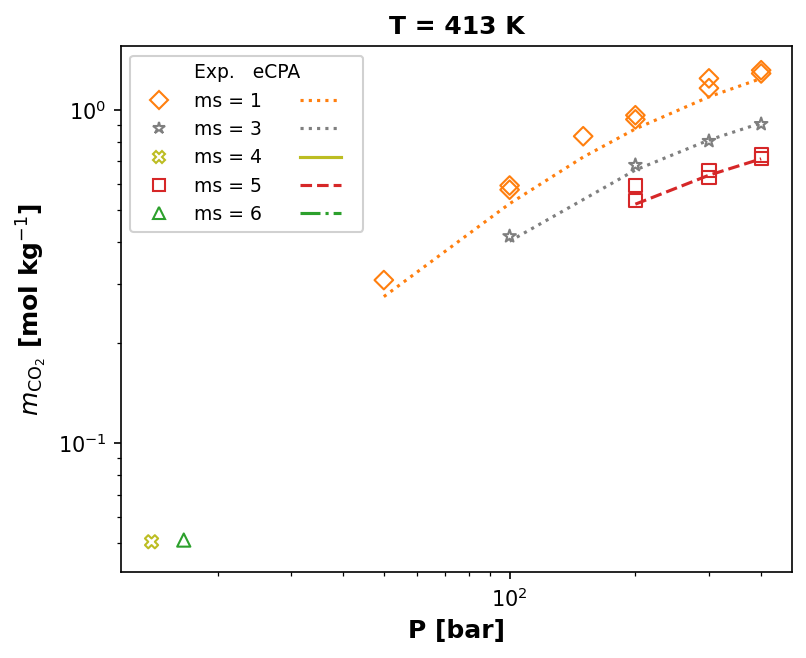
\includegraphics[width=\textwidth]{../figures/co2nacl/T413K.png}\caption{413\,K}\end{subfigure}\hfill
  \begin{subfigure}[t]{\snwsi}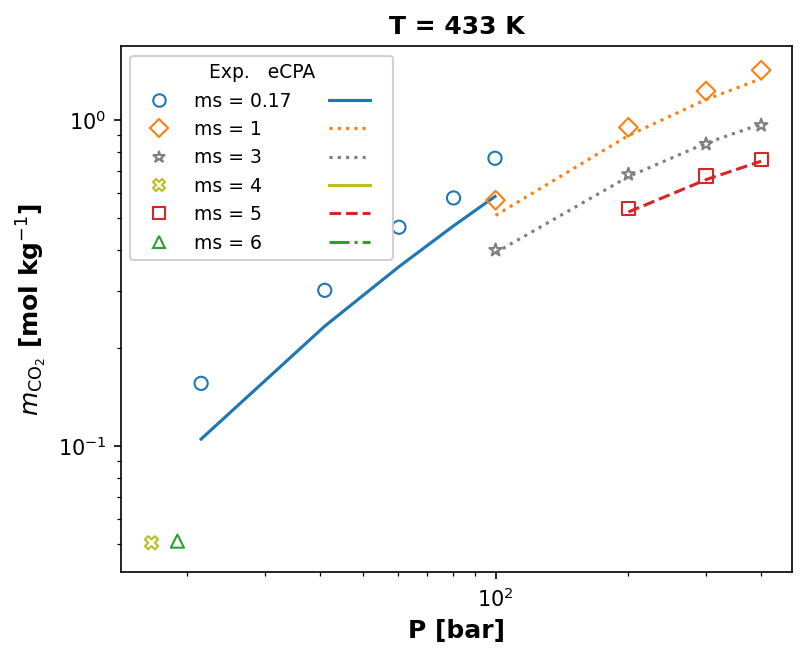
\includegraphics[width=\textwidth]{../figures/co2nacl/T433K.png}\caption{433\,K}\end{subfigure}\hfill
  \begin{subfigure}[t]{\snwsi}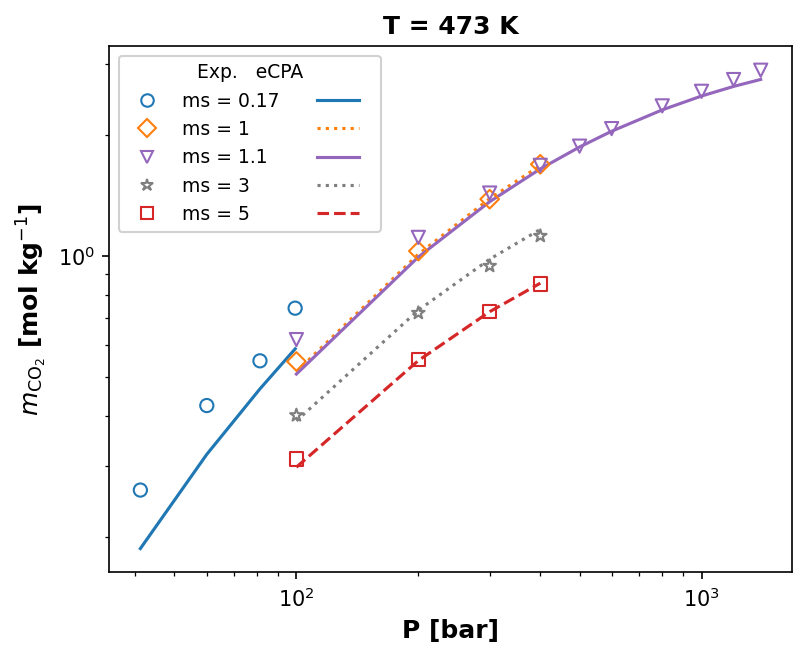
\includegraphics[width=\textwidth]{../figures/co2nacl/T473K.png}\caption{473\,K}\end{subfigure}
  \caption{CO$_2$ solubility in NaCl brine at nine representative temperatures not shown in
           Fig.~\ref{fig:co2nacl_Tpanel} (278--473\,K), including data at high NaCl molalities
           up to $m_s = 6$\,mol\,kg$^{-1}$ from multiple sources.
           Each panel shows CO$_2$ molality $m_c$ [mol\,kg$^{-1}$] vs.\ pressure (log--log).
           Open symbols: experimental data; lines: eCPA.
           Colors and markers distinguish NaCl molalities (see legend).}
  \label{fig:co2nacl_Tpanel_SI}
\end{figure}

%% --- SI Figure S3: high-T CO2+NaCl panels (T=573K, 623K) ---
\begin{figure}[h!]
  \centering
  \newcommand{\snwhighT}{0.46\textwidth}%
  \begin{subfigure}[t]{\snwhighT}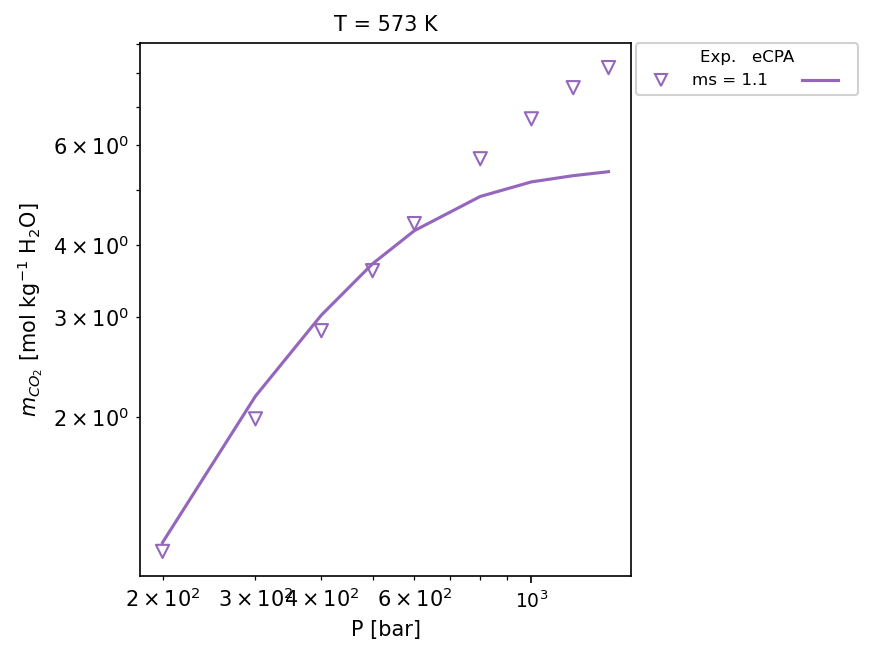
\includegraphics[width=\textwidth]{../figures/co2nacl/T573K.png}\caption{573\,K}\end{subfigure}\hfill
  \begin{subfigure}[t]{\snwhighT}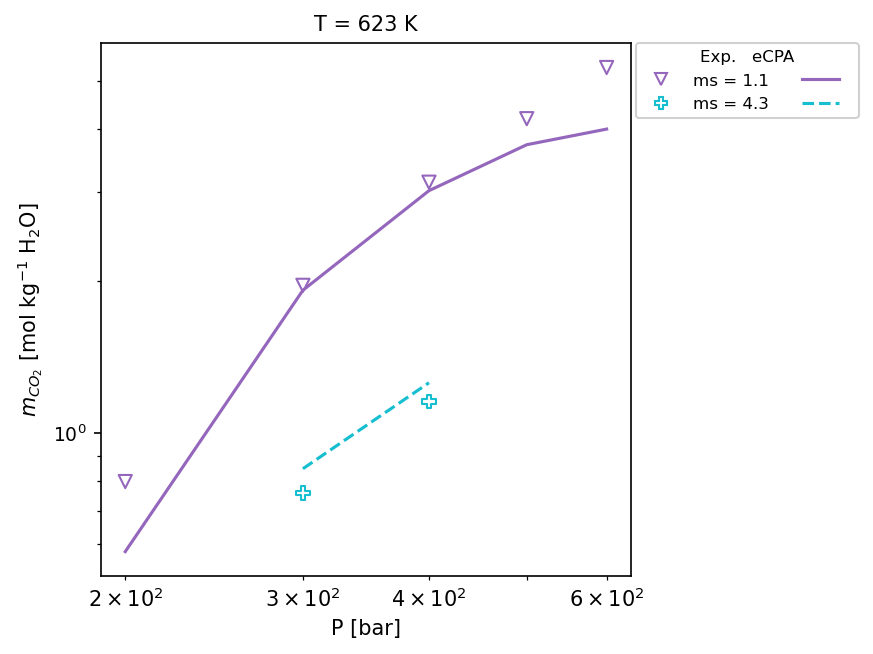
\includegraphics[width=\textwidth]{../figures/co2nacl/T623K.png}\caption{623\,K}\end{subfigure}
  \caption{CO$_2$ solubility in NaCl brine at hydrothermal temperatures
           (a) $T = 573$\,K, (b) $T = 623$\,K.
           Each panel shows CO$_2$ molality $m_c$ [mol\,kg$^{-1}$] vs.\ pressure.
           Open symbols: experimental data \citep{Takenouchi1965}; lines: eCPA.
           At $T \geq 673$\,K, eCPA predicts single-phase (fully miscible) behavior
           for all available experimental pressures (300--900\,bar).}
  \label{fig:co2nacl_highT_SI}
\end{figure}

\section*{Open-Source Code Description}

\section{Software Overview}
\label{sec:si_overview}

All code is written in Python 3.11+ and depends on NumPy \citep{Harris2020},
SciPy \citep{Virtanen2020}, pandas \citep{McKinney2010}, and matplotlib.
The repository is structured as a single directorycontaining an
importable \texttt{ecpa/} package and a set of runner scripts.

\medskip
\noindent\textbf{Repository root:} 

\subsection{Core package: \texttt{ecpa/}}
\label{sec:si_ecpa}

\subsubsection{\texttt{ecpa/constants.py}}
Physical constants, molecular weights, critical properties, CPA/eCPA EoS parameters
(co-volumes, Soave parameters, association parameters, ion parameters, Debye--Hückel
distances, Born radii, NRTL ion--molecule energy parameters, temperature-dependent binary
interaction coefficients), and Péneloux volume shifts.
Also defines the relative permittivity model constants (Onsager--Kirkwood parameters,
dipole moments, polarizabilities).
All values are scalars; three Péneloux shift constants are provided:
\texttt{Penelouxs} (NaCl, from \citet{Coelho2025}),
\texttt{Peneloux\_H2O} (H$_2$O, optimized in this work),
\texttt{Peneloux\_CO2} (CO$_2$, default 0).

\subsubsection{\texttt{ecpa/parameters.py}}
Assembles all constants from \texttt{constants.py} into a single \texttt{params} dict of
\texttt{np.float64} scalars, which is passed to all EoS computation functions.
The function \texttt{make\_params()} is the standard entry point for all downstream code.

\subsubsection{\texttt{ecpa/elv.py}}
Implements the equilibrium-liquid-vapor (ELV) residual system \texttt{ELV(sol, T, P, ms, params)}
whose ten-vector root corresponds to the simultaneous solution of:
fugacity equalities for H$_2$O and CO$_2$ between phases;
cubic compressibility factors $Z_w$ and $Z_c$ for both phases;
the Wertheim association fractions $\chi_{1w}$ and $\chi_{1c}$;
the relative permittivity $\varepsilon_r$ (aqueous phase);
and three derivative quantities needed for warm-starting.
Also provides the Jacobian \texttt{ELV\_jac} via complex-step differentiation
(\texttt{USE\_COMPLEX\_JAC} flag).

\subsubsection{\texttt{ecpa/flash.py}}
Main flash routines:
\begin{itemize}
  \item \texttt{flash\_co2\_h2o\_salt\_ssi(T, P, z, ms, params, ...)}: robust cold-start
        SSI flash for the ternary system. Solves the Rachford--Rice equation at each step,
        iterates K-values with damping $\omega = 0.7$, falls back to Newton if SSI stalls.
        Returns phase compositions, compressibility factors, and convergence diagnostics.
  \item \texttt{flash\_co2\_h2o\_salt\_fast(T, P, z, ms, params, guess\_fn, ...)}: fast flash
        using the solution table for initialization (Section~\ref{sec:fast_flash}).
        Selectively skips the Michelsen stability test for pre-classified two-phase conditions;
        uses $\omega = 1.0$ for warm-started SSI.
        Falls back to cold-start SSI on failure.
\end{itemize}

\subsubsection{\texttt{ecpa/stability.py}}
Phase stability routines:
\begin{itemize}
  \item \texttt{ecpa\_stability(T, P, z, ms, params)}: full Michelsen TPD test.
        Returns the minimum TPD value, the trial phase composition at the minimum,
        and a convergence flag.
        Two trial phases are tested (CO$_2$-rich initialization for both, with different
        initial K-value multipliers), and the lower TPD result is taken.
  \item \texttt{stability\_map(T\_range, P\_range, z, ms, params, n\_workers)}: parallel
        stability scan on a 2D $(T, P)$ grid.
        Used for generating phase envelopes and stability maps (notebook Section~7.5).
  \item \texttt{stability\_ms\_scan(T, P\_range, ms\_range, z, params)}: serial
        warm-started $P$-scan for each $m_s$ value.
        Used for the salinity-dependence plot (notebook Section~7.6).
\end{itemize}

\subsubsection{\texttt{ecpa/solution\_table.py}}
Builds and manages the four-dimensional solution table:
\begin{itemize}
  \item \texttt{build\_solution\_table(T\_grid, logP\_grid, z\_grid, ms\_grid, params,
        n\_workers, ...)}: runs the full flash at each grid point using multiprocessing
        (\texttt{spawn} context), with T-continuation and $m_s$-continuation as fallbacks.
        Returns arrays \texttt{sol\_filled}, \texttt{ms\_aq\_filled}, and \texttt{stable}.
        Saves to \texttt{results/solution\_table.npz}.
  \item \texttt{make\_solution\_guess\_fn(T\_grid, logP\_grid, z\_grid, ms\_grid, sol, stable)}:
        constructs a \texttt{RegularGridInterpolator} in $(T, \log_{10}P, z, m_s)$ space
        and returns a callable \texttt{guess\_fn(T, P, z, ms)} that returns the interpolated
        10-vector initial guess and the two-phase stability hint.
\end{itemize}

\subsubsection{\texttt{ecpa/scan.py}}
\texttt{scan\_flash(T\_vals, P\_vals, z\_vals, ms\_vals, params, ...)}:
Structured grid scan calling \texttt{flash\_co2\_h2o\_salt\_ssi} at each point.
Results are cached in \texttt{results/scan\_results.parquet} (Parquet format for efficient
column-oriented storage and fast reload).
Used to populate the solution table and to generate the phase diagrams shown in the paper.

\subsubsection{\texttt{ecpa/envelope.py}}
\texttt{find\_envelope\_from\_scan(scan\_df, params, guess\_fn, n\_workers)}:
Identifies phase-boundary transitions from the scan grid and refines each to the exact
two-phase boundary by bisection in $P$ at fixed $T$.
Parallelized using \texttt{multiprocessing} (spawn context) with worker-global EoS state
via \texttt{\_envelope\_worker\_init}.

\subsubsection{\texttt{ecpa/guess\_table.py}}
Manages an alternative lookup table built from a pre-existing high-resolution CPA binary
database (\texttt{CPA\_ELV\_all.parquet}):
\begin{itemize}
  \item \texttt{load\_cpa\_guess\_table()}: reads and groups the Parquet database by temperature.
  \item \texttt{make\_guess\_fn(groups, temps)}: returns a callable that returns a warm-start
        guess via bilinear $(T, P)$ interpolation.
        Used as a fallback initialization for the ternary flash when the 4D table is not
        loaded.
\end{itemize}

\subsubsection{\texttt{ecpa/validate\_co2h2o.py}}
CO$_2$ + H$_2$O binary VLE validation:
\begin{itemize}
  \item \texttt{load\_co2h2o\_exp()}: parses all \texttt{EXP/CO2-WATER/*.txt} files with
        $x_{\text{CO}_2}$ or $y_{\text{H}_2\text{O}}$ columns; returns a long-format DataFrame.
  \item \texttt{run\_validation(exp\_df, params, ...)}: runs \texttt{flash\_co2\_h2o\_salt\_fast}
        at each experimental condition ($m_s = 10^{-4}$\,mol\,kg$^{-1}$) for eCPA and
        \texttt{CPA2.flash\_co2\_h2o\_tpz} for the salt-free CPA.
  \item \texttt{compute\_metrics(results)}: AARE, RMSE, and bias grouped by temperature
        and model.
  \item \texttt{plot\_co2h2o\_T\_figures(results, fig\_dir)}: generates per-temperature
        figures in the two-panel format (left: $x_{\text{CO}_2}$; right: $y_{\text{H}_2\text{O}}$).
\end{itemize}

\subsubsection{\texttt{ecpa/validate\_nacl.py}}
CO$_2$ + NaCl VLE validation:
\begin{itemize}
  \item \texttt{load\_co2nacl\_exp()}: parses all \texttt{EXP/CO2-NaCl/*.txt} files
        (files with \texttt{\_X} suffix are skipped);
        returns a long-format DataFrame with columns
        \texttt{T\_K}, \texttt{P\_bar}, \texttt{ms}, \texttt{qty}, \texttt{exp\_value}.
        Three quantity types are handled: \texttt{mc} (CO$_2$ molality), \texttt{xc\_W\_SALTfree},
        \texttt{xc\_W\_SALTincl}, and \texttt{xc\_C}.
  \item \texttt{run\_validation(exp\_df, guess\_table\_fn, params, T\_max, ms\_max, ...)}: runs
        the eCPA flash at each experimental condition; handles multiple $z_{\text{CO}_2}$
        candidates and falls back gracefully on convergence failure.
  \item \texttt{compute\_metrics(results)}: AARE, bias, and RMSE grouped by temperature,
        salinity range, and quantity type.
  \item \texttt{plot\_nacl\_T\_figures(results, fig\_dir, T\_max)}: per-temperature figures
        (left panel: $m_c$ [mol\,kg$^{-1}$] vs.\ $P$, log--log; right panel: $y_{\text{CO}_2}$ vs.\ $P$,
        log--linear) with per-molality color, marker, and linestyle styles, and a two-column
        legend outside the right panel.
  \item \texttt{plot\_validation\_parity(results)}: parity plot with error bands.
  \item \texttt{plot\_error\_heatmap(results)}: heatmap of absolute relative error.
\end{itemize}

\subsubsection{\texttt{ecpa/plotting.py}}
Shared plotting utilities: color palettes, axis formatting, figure saving helpers.

\subsubsection{\texttt{ecpa/exp\_data.py}}
Helpers for parsing the experimental data text files (pressure, temperature, molality,
quantity columns) from the \texttt{EXP/} directory.

\subsubsection{\texttt{ecpa/utils.py}}
Numerical utilities: root-bracketing helpers, convergence diagnostics, and a
\texttt{safe\_fsolve} wrapper that returns \texttt{NaN} on failure rather than raising.

\subsection{Salt-free CPA module: \texttt{CPA2.py}}
\label{sec:si_cpa2}

\texttt{CPA2.py} is a self-contained, single-file implementation of the salt-free CPA EoS
for the CO$_2$ + H$_2$O binary.
It uses the same Coelho eCPA parameters (\texttt{PARAM\_SET = "eCPA"}) by default.
Key functions:

\begin{itemize}
  \item \texttt{kij\_ecpa(T)}, \texttt{s14\_ecpa(T)}: evaluate the temperature-dependent
        binary interaction parameter and cross-association strength.
  \item \texttt{ChiChi(x, ep)}: solves the $2 \times 2$ association equation system for
        $(\chi_w, \chi_c)$ via a Newton step.
  \item \texttt{ZChi(A, B, x, Kapa, Eps, swc)}: solves the cubic equation for the
        compressibility factor $Z$ and the association fractions simultaneously;
        returns $(Z, \chi, \chi_1)$.
  \item \texttt{tie\_line\_two\_comp(T, P\_bar, ...)}: SSI loop for the two-component
        K-value iteration; returns converged K-values, phase compositions, $Z$-factors,
        and density.
  \item \texttt{flash\_tpz\_two\_comp(T, P\_bar, z, ...)}: TPz flash; determines the
        vapor fraction $\beta$ and classifies the state as \texttt{two\_phase},
        \texttt{single\_liquid}, \texttt{single\_vapor}, or \texttt{failed}.
  \item \texttt{flash\_co2\_h2o\_tpz(T, P\_bar, z\_co2, kij12, swc, vshift\_h2o,
        vshift\_co2, ...)}: convenience wrapper for the CO$_2$ + H$_2$O binary.
        Accepts optional Péneloux volume shifts (m$^3$\,mol$^{-1}$) applied post-flash
        to \texttt{rho\_mass} without affecting phase compositions.
\end{itemize}

\subsection{Runner scripts}
\label{sec:si_runners}

\begin{description}
  \item[\texttt{\_run\_solution\_table.py}]
        Rebuilds the 4D solution table from scratch.
        Calls \texttt{ecpa.solution\_table.build\_solution\_table} with the standard grid,
        then saves to \texttt{results/solution\_table.npz}.
        Requires a machine with $\geq$4 cores; typical wall time $\sim$1--4\,h depending
        on hardware.

  \item[\texttt{\_add\_ms0\_to\_solution\_table.py}]
        Adds the $m_s = 0$ slice to an existing solution table by bilinear interpolation
        from the binary database \texttt{CPA\_ELV\_all.parquet}, without re-running the
        full flash.

  \item[\texttt{\_extend\_solution\_table\_high\_T.py}]
        Extends the solution table from 523\,K to 623\,K via ELV solves with T-continuation
        at $m_s = 0$, followed by $m_s$-continuation up to $m_s = 3.0$\,mol\,kg$^{-1}$.

  \item[\texttt{\_extend\_solution\_table\_full.py}]
        Extends the solution table in two phases: (1) adds $m_s$ levels 3.5--6.0\,mol\,kg$^{-1}$
        for all existing $T$ values via $m_s$-continuation from the $m_s = 3.0$ solution;
        (2) adds $T$ levels 638--728\,K for all $m_s$ levels via T-continuation from 623\,K,
        then $m_s$-continuation.
        Run after \texttt{\_extend\_solution\_table\_high\_T.py}.

  \item[\texttt{\_run\_validation\_full.py}]
        Runs the CO$_2$ + NaCl validation over all experimental conditions ($T = 278$--$723$\,K,
        $m_s = 0.17$--$6.0$\,mol\,kg$^{-1}$) using \texttt{flash\_co2\_h2o\_salt\_fast} with
        the extended solution table.  Saves \texttt{results/validation\_co2nacl.parquet} and
        all figures in \texttt{figures/co2nacl/}.

  \item[\texttt{\_run\_validation\_co2h2o.py}]
        Analogous runner for the CO$_2$ + H$_2$O binary.
        Saves \texttt{results/validation\_co2h2o.parquet} and figures in
        \texttt{figures/co2h2o/}.

  \item[\texttt{\_run\_smooth\_salty.py}]
        Computes eCPA smooth curves at $m_s = 0.5$, 1.0, 2.0\,mol\,kg$^{-1}$ over a dense
        pressure grid (no experimental data required) and regenerates the CO$_2$ + H$_2$O
        figures with the salty curves overlaid.

  \item[\texttt{\_validate\_density\_co2h2o.py}]
        Validates CPA and eCPA aqueous-phase density predictions against experimental data.
        Reads Péneloux shifts from \texttt{ecpa/constants.py} via \texttt{make\_params()};
        uses direct ELV Newton solves (not table interpolation) to avoid artefacts near the
        CO$_2$ critical region.
        Generates per-temperature density figures and a parity plot.

  \item[\texttt{\_run\_benchmark.py}]
        Benchmarks cold-start SSI vs.\ warm-started fast flash at a representative
        $(T, z, m_s)$ point over 30 pressure values.
        Reports mean iterations, wall time, and speedup factor.

  \item[\texttt{\_replot\_co2nacl.py}]
        Regenerates CO$_2$ + NaCl per-temperature figures from a saved Parquet file
        without re-running the flash.

  \item[\texttt{\_replot\_co2h2o.py}]
        Analogous replot script for the CO$_2$ + H$_2$O binary.

  \item[\texttt{co2brine\_simulator.py}]
        Minimal isothermal IMPEC compositional reservoir simulator demonstrating
        integration of \texttt{flash\_co2\_h2o\_salt\_fast} in a time-stepping loop.
        Implements TPFA pressure solve, CFL-limited explicit transport, and
        parallel flash dispatch via \texttt{multiprocessing}.
        Runs a five-spot injection scenario on a $50\times50$ Cartesian grid.

  \item[\texttt{\_run\_simulator\_paper.py}]
        Runs the simulator and generates the paper-quality figures for
        Section~\ref{sec:simulator}: the three-panel $S_g$ evolution figure and
        the flash performance figure.
        Saves timing statistics to \texttt{results/simulator\_timing.npz}.
\end{description}

\subsection{Interactive notebook: \texttt{eCPA\_notebook.ipynb}}
\label{sec:si_notebook}

A Jupyter notebook provides an interactive interface to all major functions:

\begin{center}
\begin{tabular}{ll}
  \toprule
  Section & Content \\
  \midrule
  7.1 & Flash at a single $(T, P, z, m_s)$ point \\
  7.2 & Fugacity equality verification \\
  7.3 & Stability sum $\Sigma_W$ vs.\ $P$ \\
  7.4 & Phase envelope plot \\
  7.5 & 2D stability map (parallel grid) \\
  7.6 & Salinity scan (\texttt{stability\_ms\_scan}) \\
  8.1 & Build / load the solution table \\
  8.2 & Build the interpolating \texttt{guess\_fn} \\
  8.3 & Benchmark: fast flash vs.\ cold SSI \\
  \bottomrule
\end{tabular}
\end{center}

\subsection{Experimental data directory: \texttt{EXP/}}
\label{sec:si_data}

\begin{description}
  \item[\texttt{EXP/CO2-WATER/}] Binary CO$_2$ + H$_2$O VLE data.
        Each file \texttt{EXP*\_T\{T\}K.txt} contains a header with a literature reference,
        column names, and tab-separated data rows.
        Columns include \texttt{P [bar]}, \texttt{xc\_W [SALTfree]} or \texttt{mc [mol/kg]},
        and optionally \texttt{yc\_C}, \texttt{rho\_W} (aqueous density), and \texttt{rho\_C}
        (CO$_2$-rich density).
        Files with \texttt{\_X} suffix are excluded from validation.
  \item[\texttt{EXP/CO2-NaCl/}] Ternary CO$_2$ + H$_2$O + NaCl VLE data.
        Same file format; \texttt{ms} column gives the NaCl molality.
\end{description}

\subsection{Results and figures}
\label{sec:si_results}

\begin{description}
  \item[\texttt{results/solution\_table.npz}] 4D solution table
        (24T $\times$ 30P $\times$ 18$z$ $\times$ 8$m_s$ $\times$ 10 solution variables
        + stable flag). Backed up before each extension.
  \item[\texttt{results/validation\_co2h2o.parquet}] 631-row table of CO$_2$ + H$_2$O
        validation results.
  \item[\texttt{results/validation\_co2nacl.parquet}] 423-row table of CO$_2$ + NaCl
        validation results.
  \item[\texttt{results/density\_co2h2o.parquet}] 37-row table of aqueous-phase density
        predictions.
  \item[\texttt{figures/co2h2o/}] Per-temperature VLE figures for the binary.
  \item[\texttt{figures/co2nacl/}] Per-temperature VLE figures for the ternary.
  \item[\texttt{figures/density/}] Per-temperature and parity density figures.
\end{description}

\end{document}
